\chapter{พื้นฐาน}
\label{chapter: background}

\begin{Parallel}[c]{0.54\textwidth}{0.4\textwidth}
	\selectlanguage{english}
	\ParallelLText{
		``Divide each difficulty into as many parts as is feasible and necessary to resolve it.''\\
		---Ren\'e Descartes
	}
	\selectlanguage{thai}
	\ParallelRText{
		``แตกปัญหาออกเป็นส่วนย่อย ๆ เท่าที่จะทำได้และจำเป็นที่จะแก้มันได้'' \\
		---เรอเน เดการ์ต
	}
\end{Parallel}
\index{english}{words of wisdom!Ren\'e Descartes}
\index{english}{quote!break down the problem}
\vspace{0.5cm}

ศาสตร์การรู้จำรูปแบบและการเรียนรู้ของเครื่อง อาศัยพื้นฐานจากหลาย ๆ ศาสตร์
การทำความเข้าใจศาสตร์นี้
และพัฒนาการ
จำเป็นต้องอาศัยศาสตร์พื้นฐาน.
บทนี้จะทบทวนศาสตร์พื้นฐานที่สำคัญ คือ พีชคณิตเชิงเส้น ความน่าจะเป็น และการหาค่าดีที่สุด.

\section{พีชคณีตเชิงเส้น}
\label{sec: linear algebra}
\index{english}{linear algebra}
\index{english}{revise!linear algebra}
\index{thai}{พีชคณีตเชิงเส้น}
\index{thai}{ทบทวน!พีชคณีตเชิงเส้น}


การรู้จำรูปแบบและการเรียนรู้ของเครื่อง เกี่ยวข้องกับข้อมูลและตัวแปรจำนวนมาก.
พีชคณีตเชิงเส้น%
\footnote{%
เนื้อหาในหัวข้อนี้ ได้รับอิทธิพลหลักจาก
\cite{GoodfellowEtAl2016}
\cite{ChongZak2ndEd}
และ
\cite{Strang2016}
}
มีเครื่องมือและทฤษฎีต่าง ๆ 
ที่ช่วยอำนวยความสะดวก
ในทำงานกับตัวแปรจำนวนมาก
ดังนั้น จึงเป็นเป็นพื้นฐานที่สำคัญ

\textbf{สเกล่าร์} (scalar) 
\index{english}{scalar}
\index{thai}{สเกล่าร์}
หมายถึง ตัวเลขเดี่ยว เช่น ตัวเลข $3$ ตัวเลข $0$ ตัวเลข $-0.42$ ตัวเลข $168.79$.
กำหนดให้ $\mathbb{R}$ แทนเซตของจำนวนจริง.
ดังนั้น สัญกรณ์ เช่น $x \in \mathbb{R}$ ระบุว่า ตัวแปร $x$ เป็นสเกล่าร์ของจำนวนจริง.

\textbf{เวกเตอร์} (vector) 
\index{thai}{เวกเตอร์}
\index{english}{vector}
หมายถึง ลำดับของตัวเลข.
เวกเตอร์ ในพีชคณีตเชิงเส้น มีสองชนิด 
คือ เวกเตอร์แนวนอน และเวกเตอร์แนวตั้ง. 
เวกเตอร์แนวนอน
แสดงด้วยลำดับในแนวนอน เช่น\\  $[103.4, \; -28.6, \; 0, \; 9.99]$ เป็นเวกเตอร์แนวนอน ที่เป็นลำดับของตัวเลขสี่ตัว.
ตำราเล่มนี้จะใช้เวกเตอร์แนวตั้งเป็นหลัก
นั่นคือ หากกล่าวถึง เวกเตอร์ โดยไม่ได้ระบุเฉพาะเจาะจงแล้ว จะหมายถึง เวกเตอร์แนวตั้ง ที่แสดงด้วยลำดับในแนวตั้ง 
ดังแสดงใน
สมการ~\ref{eq: linalg vector}
%
\begin{eqnarray}
\bm{x} = \begin{bmatrix}
x_1 \\
x_2 \\
\vdots \\
x_n
\end{bmatrix}
\label{eq: linalg vector}
\end{eqnarray}
เมื่อ $x_1, \ldots, x_n$ แทนตัวเลขสเกล่าร์
และ $x_i$ เรียกว่าเป็น \textit{ส่วนประกอบ}ที่ $i$ ของเวกเตอร์ $\bm{x}$.
%
สัญกรณ์ เช่น $\bm{x} \in \mathbb{R}^n$ ระบุว่า ตัวแปร $\bm{x}$ เป็นเวกเตอร์
ที่มีส่วนประกอบจำนวน $n$ ตัว 
%(อาจเรียกว่า เวกเตอร์สัดส่วน $n$)
ซึ่ง\textit{ส่วนประกอบ}แต่ละตัวเป็นจำนวนจริง.
หมายเหตุ 
สัญลักษณ์ $\bm{0}$ หมายถึง
เวกเตอร์ที่ส่วนประกอบทุกตัวเป็นศูนย์.
นั่นคือ $\bm{0} = [0, 0, \ldots, 0]^T$.

\textbf{เมทริกซ์} (matrix)
\index{english}{matrix}
\index{thai}{เมทริกซ์}
หมายถึง โครงสร้างสองมิติของลำดับของตัวเลข
ดังแสดงในสมการ~\ref{eq: linalg matrix}
%
\begin{eqnarray}
\bm{A} = \begin{bmatrix}
A_{11} & A_{12} & \cdots & A_{1n} \\
A_{21} & A_{22} & \cdots & A_{2n} \\
\vdots & \vdots & \ddots & \vdots \\
A_{m1} & A_{m2} & \cdots & A_{mn} \\
\end{bmatrix}
\label{eq: linalg matrix}
\end{eqnarray}
เมื่อ $\bm{A}$ เป็นเมทริกซ์ขนาดมิติ $m \times n$ และ $A_{11}, \ldots, A_{mn}$ แทนตัวเลขสเกล่าร์ และ $A_{ij}$ เป็น \textit{ส่วนประกอบ}ของเมทริกซ์ ที่ดัชนีตำแหน่ง แถว $i$ และสดมภ์ $j$.
ดัชนี อาจเขียนโดยใช้ตัวห้อย โดยมีเครื่องหมายจุลภาคคั่น เช่น $A_{i,j}$
หรือเครื่องหมายจุลภาคคั่นอาจถูกละไว้ได้
เช่น $A_{ij}$ ในกรณีที่ความหมายชัดเจน.
%
เมทริกซ์สามารถถูกระบุขนาดมิติ ได้จาก
สัญกรณ์ $\bm{A} \in \mathbb{R}^{m \times n}$.

นอกจากนี้ ศาสตร์การเรียนรู้ของเครื่อง 
นิยมใช้สัญกรณ์จุดคู่ ดังปฏิบัติใน \cite{GoodfellowEtAl2016}.
นั่นคือ กำหนดให้
สัญกรณ์ $\bm{A}_{i,:}$ 
\index{english}{colon notation}
\index{thai}{สัญกรณ์จุดคู่}
หมายถึง เมทริกซ์ย่อย ที่ได้จาก\textit{ส่วนประกอบ}ที่แถว $i$ ของเมทริกซ์ $\bm{A}$ 
คือ
$\bm{A}_{i,:} = [A_{i1}, \; A_{i2}, \; \ldots, \; A_{in}]$
เรียกว่า แถว $i$ ของ $\bm{A}$.
ทำนองเดียวกัน
สัญกรณ์ $\bm{A}_{:,j}$ หมายถึง เมทริกซ์ย่อย ที่ได้จาก\textit{ส่วนประกอบ}ที่สดมภ์ $j$ ของเมทริกซ์ $\bm{A}$ เรียกว่า สดมภ์ $j$ ของ $\bm{A}$.

\textbf{การสลับเปลี่ยน} (transpose)
\index{english}{transpose}
\index{thai}{การสลับเปลี่ยน}
เป็นการดำเนินการจัดเรียงลำดับใหม่.
%
สำหรับเวกเตอร์
การสลับเปลี่ยนของเวกเตอร์แนวนอน จะได้เวกเตอร์แนวตั้ง
และการสลับเปลี่ยนของเวกเตอร์แนวตั้ง จะได้เวกเตอร์แนวนอน
และใช้สัญกรณ์ เช่น $\bm{x}^T$ คือ การสลับเปลี่ยนของเวกเตอร์ $\bm{x}$
เช่น จากสมการ~\ref{eq: linalg vector} เวกเตอร์ $\bm{x}^T = [x_1, \; x_2, \; \ldots, \; x_n]$
หรือ ในทางกลับกัน สมการ~\ref{eq: linalg vector} อาจเขียนใหม่ได้ในรูป
$\bm{x} = [x_1, \; x_2, \; \ldots, \; x_n]^T$

สำหรับเมทริกซ์ 
การสลับเปลี่ยนของเมทริกซ์ ซึ่งใช้สัญกรณ์ เช่น $\bm{A}^T$
คือ การเปลี่ยนตำแหน่งของส่วนประกอบ
โดย ส่วนประกอบที่ตำแหน่ง $(i,j)$ จะถูกเปลี่ยนไปอยู่ตำแหน่ง $(j,i)$
ซึ่งผลที่ได้เสมือนกับการสลับตำแหน่งรอบแนวทะแยงมุมของเมทริกซ์.
สมการ~\ref{eq: linalg transpose}
แสดงการสลับเปลี่ยนของเมทริกซ์ $\bm{A}$.
% 
\begin{eqnarray}
\bm{A}^T = \begin{bmatrix}
A_{11} & A_{21} & \cdots & A_{m1} \\
A_{12} & A_{22} & \cdots & A_{m2} \\
\vdots & \vdots & \ddots & \vdots \\
A_{1n} & A_{2n} & \cdots & A_{mn} \\
\end{bmatrix}
\label{eq: linalg transpose}
\end{eqnarray}
%
การสลับเปลี่ยนของเมทริกซ์ จะทำให้ขนาดมิติของเมทริกซ์เปลี่ยนไป
เช่น จากตัวอย่าง ขนาดมิติของเมทริกซ์ $\bm{A}$ คือ $m \times n$ 
แต่
ขนาดมิติของเมทริกซ์ $\bm{A}^T$ คือ $n \times m$ (สังเกตจาก $\bm{A}^T$ มี $n$ แถว และ $m$ สดมภ์)



\paragraph{มิติ และลำดับชั้น.}
\index{english}{dimension}
\index{thai}{มิติ}
\index{english}{rank}
\index{thai}{ลำดับชั้น}
โครงสร้างของเวกเตอร์ มีหนึ่งมิติของลำดับ ในลักษณะที่ลำดับของข้อมูลดำเนินไปได้แนวเดียว.
โครงสร้างของเมทริกซ์ มีสองมิติ ในลักษณะที่ลำดับของข้อมูลดำเนินไปได้สองแนว.
ภาพขาวดำ%
\footnote{%
ภาพขาวดำ ในบริบททั่วไป 
หมายถึง ภาพสเกลเทา
ที่ในภาพสามารถแสดงค่าน้ำหนักระดับสีต่าง ๆ ได้ตั้งแต่ขาว ไปจนถึงดำ.
อย่างไรก็ตาม
ในระบบข้อมูล มีข้อมูลภาพที่เป็นค่าทวิภาค
นั่นคือ 
ภาพจะสามารถแสดงสีได้แค่สองสี นั่นคือ แต่ละพิกเซล จะสามารถแสดงได้แค่สีขาว หรือสีดำ เท่านั้น ไม่สามารถแสดงระดับสีอื่น ๆ ระหว่างกลางได้.
ดังนั้น เพื่อลดความสับสน ในที่นี้จะใช้คำว่า ภาพสเกลเทา แทนคำว่า ภาพขาวดำ.
}%
หรือภาพสเกลเทา (gray-scale image) ก็มีลักษณะโครงสร้างสองมิติของลำดับ
นั่นคือ มีโครงสร้างสองมิติของลำดับค่าพิกเซล ตามลำดับแนวตั้ง และตามลำดับแนวนอน.
การเขียนโปรแกรมจะใช้โครงสร้างข้อมูล เช่น อาร์เรย์ (array) ขนาดสองมิติ ในการแทนข้อมูลภาพสเกลเทานี้.

ข้อมูลอาจมีโครงสร้างมิติของลำดับที่ซับซ้อนมากได้.
%
ภาพสี (color image) มีโครงสร้างสามมิติของลำดับค่าพิกเซล ตามลำดับแนวตั้ง ตามลำดับแนวนอน
และตามชุดของช่องสี แดง เขียว น้ำเงิน.
(แม้ช่องสีไม่ได้มีความสัมพันธ์ในเชิงลำดับ ในลักษณะที่ช่องสีแดง ไม่จำเป็นต้องมาก่อนช่องสีเขียว เป็นต้น
แต่ข้อมูลของช่องสีต่าง ๆ แยกออกเป็นลักษณะของตัวเอง).
การเขียนโปรแกรมจะใช้โครงสร้างข้อมูล เช่น อาร์เรย์ ขนาดสามมิติ ในการแทนข้อมูลภาพสี.
%
ข้อมูลวิดีโอ (video)
เป็นข้อมูลเป็นลักษณะโครงสร้างสี่มิติของลำดับค่าพิกเซล
ตามลำดับแนวตั้ง ตามลำดับแนวนอน
ตามชุดของช่องสี และตามลำดับเวลา.
การเขียนโปรแกรมจะใช้โครงสร้างข้อมูล เช่น อาร์เรย์ ขนาดสี่มิติ ในการแทนข้อมูลวิดีโอ
และข้อมูลวิดีโอ ที่กล่าวถึงนี้ ยังไม่ได้รวมข้อมูลช่องเสียงด้วย
ซึ่งหากเป็นช่องเสียงเดี่ยว (monophonic sound channel) ก็ต้องการมิติของอาร์เรย์อีกหนึ่งมิติ
หรือหากเป็นช่องเสียงสเตอริโอ (steriophonic sound channel) ก็ต้องการมิติของอาร์เรย์อีกสองมิติ
หรือหากแยกช่องเสียงพูด ออกจากเสียงประกอบอื่น ๆ
หรือมีข้อมูลคำบรรยายภาษาต่าง ๆ ประกอบ ก็ต้องการมิติของอาร์เรย์เพิ่มขึ้นอีก.
%

อย่างไรก็ตาม หากกล่าวถึง ``มิติ'' นั้นจะสังเกตว่า
ภาพสเกลเทาสองมิติ เป็นข้อมูลโครงสร้างลำดับสองมิติ.
ภาพสีสองมิติ เป็นข้อมูลโครงสร้างลำดับสามมิติ.
วิดีโอ (ของภาพสองมิติไม่รวมข้อมูลเสียง) %ไม่ใช่ของภาพสามมิติ หรือไม่ใช่ของภาพสี่มิติ ในความหมายแบบที่โรงภาพยนต์ใช้)
เป็นข้อมูลโครงสร้างลำดับสี่มิติ.
%
นอกจากนั้น เมื่อกล่าวถึง \textbf{ปริภูมิค่า} (vector space)
\index{english}{vector space}
\index{thai}{ปริภูมิค่า}
 ซึ่ง ใช้บอกถึง \textit{ขนาดความเป็นไปได้}ของลักษณะข้อมูล
และ
มิติของปริภูมิจะใช้บอกขนาด และความซับซ้อนของปริภูมินั้น ๆ
เช่น ข้อมูลสเกล่าร์ที่เป็นค่าจริง จะมีปริภูมิค่า เป็น $\mathbb{R}$ เป็นปริภูมิค่าหนึ่งมิติ.
แต่ละจุดข้อมูล อ้างถึงได้ด้วยตัวเลขตัวเดียว.
การค้นหาจุดข้อมูลที่สนใจ ในปริภูมิ ทำได้โดยการค้นหาบนเส้นจำนวนจริง.
%
ข้อมูลเวกเตอร์ที่มีส่วนประกอบเป็นค่าจริงสองค่า จะมีปริภูมิค่า เป็น $\mathbb{R}^2$.
แต่ละจุดข้อมูล อ้างถึงได้ด้วยตัวเลขสองตัว.
การค้นหาจุดข้อมูลที่สนใจ ในปริภูมิ
ทำได้โดยการค้นหาบนระนาบจำนวนจริง.
%
ข้อมูลเวกเตอร์ที่มีส่วนประกอบเป็นค่าจริงสี่ค่า จะมีปริภูมิค่า เป็น $\mathbb{R}^4$.
แต่ละจุดข้อมูล อ้างถึงได้ด้วยตัวเลขสี่ตัว.
การค้นหาจุดข้อมูลที่สนใจ ในปริภูมิ
ทำได้โดยการค้นหาในปริภูมิขนาดสี่มิติ.
%
ข้อมูลเมทริกซ์ขนาด $2 \times 2$ จะมีปริภูมิค่า เป็น $\mathbb{R}^{2\times2}$.
แต่ละจุดข้อมูล อ้างถึงได้ด้วยตัวเลขสี่ตัว.
การค้นหาจุดข้อมูลที่สนใจ ในปริภูมิ
ทำได้โดยการค้นหาบนปริภูมิขนาดสี่มิติ 
เช่นเดียวกับ ข้อมูลเวกเตอร์ที่มีส่วนประกอบสี่ค่าจริง.
นั่นคือ เวกเตอร์ที่มีส่วนประกอบสี่ค่าจริง มีความสามารถในการแทนข้อมูลเทียบเท่ากับ
เมทริกซ์ขนาด $2 \times 2$
เพียงแต่ ข้อมูลที่เก็บในเวกเตอร์ที่มีส่วนประกอบสี่ค่าจริง
ไม่ได้มีโครงสร้างลำดับ เหมือนกับ
ข้อมูลที่เก็บในเมทริกซ์ขนาด $2 \times 2$
และโครงสร้างลำดับเช่นนี้ โดยเฉพาะหากเป็นโครงสร้างตามธรรมชาติของข้อมูล
สามารถนำมาใช้ในประโยชน์ และช่วยใน\textit{การรู้จำรูปแบบ}อย่างมีประสิทธิภาพได้ (ดังเช่น ที่จะได้อภิปรายในบท~\ref{chapter: Deep Learning} ต่อไป)
 
อย่างไรก็ตาม เพื่อลดความสับสน จากนี้ไป เมื่อกล่าวถึง ``มิติ'' จะมีการระบุอย่างชัดเจนว่า หมายถึง มิติในความหมายใด 
เช่น
คำว่า มิติ ใช้ในความหมาย มุมมอง ซึ่งเป็นเป็นความหมายกว้าง ๆ ของมิติ
และใช้ในความหมายของมิติโดยทั่วไป.
คำว่า \textit{มิติปริภูมิค่า} ใช้ในความหมายของ มิติของปริภูมิค่า 
และคำว่า \textbf{ลำดับชั้น} (rank) ใช้ในความหมายของ มิติของโครงสร้างลำดับ.
ตัวอย่าง  
ภาพสเกลเทาขนาด $600 \times 800$ พิกเซล เป็น
ภาพสองมิติ 
ที่เป็นข้อมูล\textit{ลำดับชั้น}สอง (มีลำดับตามแนวตั้ง และตามแนวนอน)
หรือสามารถแทนด้วย
เมทริกซ์ ขนาดมิติ $600 \times 800$
และมี\textit{มิติปริภูมิค่า} เป็น $480000$.
สัญกรณ์ $\{0, \ldots, 255\}^{600 \times 800}$ จะระบุชัดเจนทั้งจากมุมมองของลำดับชั้น และมิติปริภูมิค่า.
นอกจากนั้น สัญกรณ์นี้ยังระบุช่วงค่าที่เป็นไปได้ของข้อมูลด้วย ว่า แต่ละค่าเป็นจำนวนเต็มที่มีค่าระหว่าง $0$ ถึง $255$.
\index{thai}{มิติปริภูมิค่า}
\index{thai}{ลำดับชั้น}

\textbf{เทนเซอร์} (tensor) 
\index{english}{tensor}
\index{thai}{เทนเซอร์}
หมายถึง โครงสร้างลำดับชั้นของตัวเลข.
สเกล่าร์ คือ เทนเซอร์ ลำดับชั้นศูนย์ (rank-0 tensor).
เวกเตอร์ คือ เทนเซอร์ ลำดับชั้นหนึ่ง (rank-1 tensor).
เมทริกซ์ คือ เทนเซอร์ ลำดับชั้นสอง (rank-2 tensor).
ข้อมูลที่แทนด้วยอาร์เรย์ขนาด $n$ มิติ 
คือ เทนเซอร์ ลำดับชั้น $n$ (rank-n tensor).
ตัวเลขแต่ละตัวในเทนเซอร์ เป็น
\textit{ส่วนประกอบ}ของเทนเซอร์
และอ้างอิงได้โดยใช้ดัชนี ตามลำดับชั้น.

ตัวอย่าง เทนเซอร์ลำดับชั้นสี่ 
$\bm{A} \in \mathbb{R}^{1 \times 2 \times 2 \times 3}$ มีค่า
%
\[
\bm{A}
= \begin{bmatrix}
\begin{bmatrix}
[[1.2], \; [3]] & [[-8.7], \; [6]]
\end{bmatrix}
&
\begin{bmatrix}
[[0.9], \; [-1]] & [[4], \; [1]]
\end{bmatrix}
&
\begin{bmatrix}
[[11], \; [5]] & [[0.1], \; [0]]
\end{bmatrix}

\end{bmatrix}
\]
และ 
$A_{1,1,1,1} = 1.2$;
$A_{1,1,1,2} = 0.9$;
...
$A_{1,2,2,2} = 1$;
$A_{1,2,2,3} = 0$.

หมายเหตุ รูปแบบอักษรที่ใช้ คือ
ฟังก์ชันจะใช้สัญลักษณ์ เช่น $f$ หรือ $\sigma$ หรือ $\mathrm{calc}$ โดยไม่มีการทำแบบอักษรตัวหนา ไม่ว่าฟังก์ชันจะให้ค่าออกมาเป็นสเกล่าร์ หรือเมทริกซ์ หรือเทนเซอร์
เช่น $f: \mathbb{R} \rightarrow \mathbb{R}$
และ $\sigma: \mathbb{R}^n \rightarrow \mathbb{R}^{m_1 \times m_2 \times m_3}$
และ $\mathrm{calc}: \mathbb{R}^{n \times m} \rightarrow \mathbb{R}^q$.
สัญกรณ์ เช่น $f: \rho_1 \rightarrow \rho_2$
ระบุว่าฟังก์ชัน $f$ รับค่าตัวแปรที่อยู่ในเซต $\rho_1$ เพื่อไปทำการคำนวณ
และให้ผลลัพธ์การคำนวณออกมาเป็นค่าที่อยู่ในเซต $\rho_2$.
ตัวอย่างเช่น $g: \mathbb{R}^n \rightarrow \mathbb{R}$ จะบอกว่า 
ฟังก์ชัน $g$ รับตัวแปรเข้าเป็นเวกเตอร์ที่มี $n$ ส่วนประกอบ และจะให้ผลลัพธ์ออกมาเป็นสเกล่าร์.



\paragraph{การคำนวณเมทริกซ์.}
\index{english}{matrix operation}
\index{english}{matrix!operation}
\index{english}{matrix!addition}
\index{thai}{การคำนวณเมทริกซ์}
\index{thai}{เมทริกซ์!การคำนวณ}
\index{thai}{เมทริกซ์!การบวก}
การบวกลบเมทริกซ์กับเมทริกซ์ จะทำได้ ก็ต่อเมื่อ เมทริกซ์มีขนาดมิติเท่ากัน 
และผลลัพธ์คำนวณได้จากค่าของส่วนประกอบทั้งสองที่ตำแหน่งเดียวกัน เช่น
$\bm{C} = \bm{A} + \bm{B}$
โดย
$C_{ij} = A_{ij} + B_{ij}$.
%
การคำนวณสเกล่าร์กับเมทริกซ์
กำหนดให้ เป็นการคำนวณค่าสเกล่าร์นั้น ๆ กับส่วนประกอบของเมทริกซ์แต่ละตัว
เช่น
$\bm{D} = a \cdot \bm{B} + c$
โดย $D_{ij} = a \cdot B_{ij} + c$.
%
การคำนวณเวกเตอร์กับเวกเตอร์
และการคำนวณสเกล่าร์กับเวกเตอร์ ก็ทำในทำนองเดียวกัน.
(ดูตัวอย่าง จากแบบฝึกหัด~\ref{ex: linalg addition python})

\paragraph{การคูณกันของเมทริกซ์.} 
%
\textbf{การคูณเมทริกซ์} (matrix product)
\index{english}{matrix product}
\index{english}{matrix!multiplication}
\index{thai}{การคูณเมทริกซ์}
\index{thai}{เมทริกซ์!การคูณ}
จะดำเนินการได้ เมื่อเมทริกซ์สองเมทริกซ์ที่จะคูณกัน
ต้องมีขนาดมิติที่เข้ากันได้
นั่นคือ 
จำนวนสดมภ์ของเมทริกซ์ตัวหน้า
เท่ากับ
จำนวนแถวของเมทริกซ์ตัวหลัง
และใช้สัญกรณ์ เช่น 
$\bm{A} \bm{B}$ หรือ $\bm{A} \cdot \bm{B}$
โดย 
เมทริกซ์ $\bm{A}$ มีขนาดมิติ $m \times p$
เมทริกซ์ $\bm{B}$ มีขนาดมิติ $p \times n$
และ ผลลัพธ์ $\bm{C} = \bm{A} \cdot \bm{B}$ จะมีขนาดมิติ $m \times n$ และ $C_{ij} = \sum_k A_{ik} \cdot B_{kj}$.

นอกจากการคูณเมทริกซ์แล้ว
การดำเนินการ
\textbf{การคูณแบบตัวต่อตัว} (element-wise product หรือ Hadamard product)
\index{english}{element-wise product}
\index{thai}{การคูณแบบตัวต่อตัว}
ก็มีการใช้อย่างกว้างขวาง.
การคูณแบบตัวต่อตัว 
จะดำเนินการได้ ก็ต่อเมื่อ เมทริกซ์สองเมทริกซ์ที่จะคูณกัน
ต้องมีขนาดมิติที่เท่ากัน
และใช้สัญกรณ์ เช่น $\bm{A} \odot \bm{B}$
โดย
เมทริกซ์ $\bm{A}$ มีขนาดมิติ $m \times n$
เมทริกซ์ $\bm{B}$ มีขนาดมิติ $m \times n$
และ ผลลัพธ์ $\bm{C} = \bm{A} \odot \bm{B}$ จะมีขนาดมิติ $m \times n$ และ $C_{ij} = A_{ij} \cdot B_{ij}$.
%
การคูณกันของเวกเตอร์ จะแสดงเสมือนกับการดำเนินการเมทริกซ์ เช่น $z = \bm{x}^T \cdot \bm{y}$ เมื่อ $\bm{x}$ และ $\bm{y}$ มีสัดส่วนเท่ากัน และ $z = \sum_i x_i \cdot y_i$.
สังเกต 
$z = \bm{x}^T \cdot \bm{y} = \bm{y}^T \cdot \bm{x}$.
(ดูตัวอย่าง จากแบบฝึกหัด~\ref{ex: linalg matrix mult python})



\paragraph{คุณสมบัติของการคูณเมทริกซ์.}
\index{english}{matrix product!useful properties}
\index{thai}{การคูณเมทริกซ์!คุณสมบัติ}
การคูณเมทริกซ์
มีคุณสมบัติการกระจาย (distributive properties)
เช่น $\bm{A} (\bm{B} + \bm{C}) = \bm{A} \bm{B} + \bm{A} \bm{C}$
มีคุณสมบัติการเปลี่ยนกลุ่ม (associative properties)
เช่น $\bm{A} (\bm{B} \bm{C}) = (\bm{A} \bm{B}) \bm{C}$
แต่
การคูณเมทริกซ์ไม่มีคุณสมบัติการสลับที่.


\subsection{ระบบสมการ}
\index{english}{linear equations}
\index{thai}{ระบบสมการ}
\index{english}{linear algebra!linear equations}
\index{thai}{พีชคณิตเชิงเส้น!ระบบสมการ}
เมทริกซ์ เวกเตอร์ และการดำเนินการต่าง ๆ ที่กล่าวมา นอกจากจะช่วยการอ้างถึง และการจัดการกับข้อมูลทำได้อย่างสะดวกแล้ว
ยังอำนวยความสะดวกในการอ้างถึง และจัดการกับปัญหาระบบสมการ หรือปัญหาที่มีตัวแปรไม่ทราบค่า และสมการที่เกี่ยวข้องจำนวนมาก 
ตัวอย่าง เช่น
\begin{eqnarray}
x + y + z &=& 6
\label{eq: lin alg ex 1} \\
2 x + 2 y - z &=& 3
\label{eq: lin alg ex 2} \\
y + z &=& 5
\label{eq: lin alg ex 3}
\end{eqnarray}
เป็นระบบสมการเชิงเส้น และสามารถเขียนได้กระทัดรัด ด้วยสัญกรณ์ ของเมทริกซ์ และเวกเตอร์ ดังนี้
%
\begin{eqnarray}
\begin{bmatrix}
1 & 1 & 1 \\
2 & 2 & -1 \\
0 & 1 & 1
\end{bmatrix}
\cdot
\begin{bmatrix}
x \\
y \\
z
\end{bmatrix}
=
\begin{bmatrix}
6 \\
3 \\
5
\end{bmatrix}
\nonumber
\end{eqnarray}
และกระทัดรัดขึ้นอีก 
เป็น 
\begin{eqnarray}
\bm{A} \bm{x} = \bm{b}
\label{eq: lin alg example lin sys}
\end{eqnarray}
หาก นิยาม
\begin{eqnarray}
\bm{A} = 
\begin{bmatrix}
1 & 1 & 1 \\
2 & 2 & -1 \\
0 & 1 & 1
\end{bmatrix}
\mbox{ นิยาม }
%
\bm{x} = 
\begin{bmatrix}
x \\
y \\
z
\end{bmatrix}
\mbox{ และนิยาม }
\bm{b} =
\begin{bmatrix}
6 \\
3 \\
5
\end{bmatrix}
\label{eq: lin alg matrix example}
\end{eqnarray}

\textbf{เมทริกซ์เอกลักษณ์} (identity matrix) ที่นิยมใช้สัญญลักษณ์ $\bm{I}$ 
(หรือ $\bm{I}_n$ เมื่อต้องการระบุขนาดมิติ $n \times n$)
เป็นเมทริกซ์ที่มีค่าตามแนวทะแยงมุมเป็นหนึ่ง และค่าอื่น ๆ เป็นศูนย์ เช่น
เมทริกซ์เอกลักษณ์ ขนาดมิติ $3 \times 3$ คือ
\[
\bm{I} = 
\begin{bmatrix}
1 & 0 & 0 \\
0 & 1 & 0 \\
0 & 0 & 1
\end{bmatrix}
\]

เมทริกซ์เอกลักษณ์ มีคุณสมบัติสำคัญ 
คือ เมื่อคูณกับเมทริกซ์ใด หรือคูณกับเวกเตอร์ใด 
แล้วจะได้เมทริกซ์นั้น หรือเวกเตอร์นั้น ตัวเดิม.
นั่นคือ $\bm{A} \cdot \bm{I} = \bm{A}$.

\textbf{เมทริกซ์ผกผัน} (matrix inverse) คือ เมทริกซ์คู่คูณ ที่เมื่อคูณกับคู่ของมันแล้ว ผลลัพธ์จะได้เป็นเมทริกซ์เอกลักษณ์
ใช้สัญญลักษณ์เป็นเมทริกซ์ที่มีตัวยกลบหนึ่ง
เช่น $\bm{A}^{-1}$ หมายถึง
เมทริกซ์ผกผัน ที่เป็นคู่ผกผันกับ $\bm{A}$
นั่นคือ $\bm{A}^{-1} \cdot \bm{A} = \bm{I}$.
จากตัวอย่าง 
เมทริกซ์ผกผัน ที่เป็นคู่ของ $\bm{A}$
ในสมการ~\ref{eq: lin alg matrix example} คือ
\begin{eqnarray}
\bm{A}^{-1} = 
\begin{bmatrix}
1 & 0 & -1 \\
-0.6666667 & 0.3333333  &  1 \\
0.6666667 & -0.3333333 & 0
\end{bmatrix}
\label{eq: lin alg example inv}
\end{eqnarray}
จากเมทริกซ์ผกผัน
สมการ~\ref{eq: lin alg example lin sys} สามารถแก้ได้โดย $\bm{x} = \bm{A}^{-1} \bm{b}$
ซึ่งเมื่อแทนค่าเข้าไป จะได้
$\bm{x} = [1, \; 2, \; 3]^T$
ซึ่งหมายถึง 
ตัวแปร $x = 1$
ตัวแปร $y = 2$
และตัวแปร $z = 3$.
(ตัวอย่างวิธีการหาเมทริกซ์ผกผัน สามารถดูได้จากแบบฝึกหัด~\ref{ex: linalg mat inverse})

\paragraph{ความเป็นอิสระเชิงเส้น.}
สังเกตว่า ระบบสมการในตัวอย่างข้างต้น (สมการ~\ref{eq: lin alg ex 1} ถึง \ref{eq: lin alg ex 3}) มีสามสมการ และมี\textit{ตัวแปรที่ไม่ทราบค่า} (unknown variables) สามตัว ซึ่งทำให้เมทริกซ์สัมประสิทธิ์ $\bm{A}$ (สมการ~\ref{eq: lin alg matrix example}) มีจำนวนแถวเท่ากับจำนวนสดมภ์ ซึ่งเรียกว่า \textit{เมทริกซ์จตุรัส} (square matrix).

โดยทั่วไปแล้ว
ถ้าหากมีจำนวนสมการน้อยเกินไป (จำนวนแถวของเมทริกซ์ น้อยกว่า จำนวนสดมภ์ หรือ เมทริกซ์ที่มีสัดส่วนเตี้ยกว้าง)
คำตอบของระบบสมการจะมีได้หลายค่า
เช่น ตัวอย่างระบบสมการ
\begin{eqnarray}
x + y + z &=& 6 
\nonumber \\
2 x + 2 y - z &=& 3
\nonumber
\end{eqnarray}
จะได้ 
\begin{eqnarray}
\bm{A} = 
\begin{bmatrix}
1 & 1 & 1 \\
2 & 2 & -1 
\end{bmatrix}
\mbox{ เวกเตอร์ตัวแปร }
%
\bm{x} = 
\begin{bmatrix}
x \\
y \\
z
\end{bmatrix}
\mbox{ และเวกเตอร์ค่าคงที่ }
\bm{b} =
\begin{bmatrix}
6 \\
3 
\end{bmatrix}
\nonumber
\end{eqnarray}
ซึ่งมีคำตอบหลายชุด 
เช่น $x = 1, y = 2, z = 3$
หรือ
$x = 2, y = 1, z = 3$
หรือ
$x = 3, y = 0, z = 3$
หรือ
$x = 2.5, y = 0.5, z = 3$ เป็นต้น.
(จริง ๆ คือ ทุกชุดค่า ที่ $x + y = 3$ และ $z = 3$ สามารถเป็นคำตอบได้ทั้งหมด)

แต่หากมีจำนวนสมการน้อยเกินไป 
(จำนวนแถวของเมทริกซ์ มากกว่า จำนวนสดมภ์ หรือ เมทริกซ์ที่มีสัดส่วนสูงแคบ)
อาจจะไม่สามารถหาคำตอบของระบบสมการได้
เช่น ตัวอย่างระบบสมการ
\begin{eqnarray}
x + y + z &=& 6 
\label{eq: lin alg example long mat 1} \\
2 x + 2 y - z &=& 3
\label{eq: lin alg example long mat 2} \\
y + z &=& 5
\label{eq: lin alg example long mat 3} \\
x + z &=& 5
\label{eq: lin alg example long mat 4}
\end{eqnarray}
จะได้ 
\begin{eqnarray}
\bm{A} = 
\begin{bmatrix}
1 & 1 & 1 \\
2 & 2 & -1 \\
0 & 1 & 1 \\
1 & 0 & 1 
\end{bmatrix}
\mbox{ เวกเตอร์ตัวแปร }
%
\bm{x} = 
\begin{bmatrix}
x \\
y \\
z
\end{bmatrix}
\mbox{ และเวกเตอร์ค่าคงที่ }
\bm{b} =
\begin{bmatrix}
6 \\
3 \\
5 \\
5 
\end{bmatrix}
\nonumber
\end{eqnarray}
ซึ่งไม่สามารถหาคำตอบของสมการได้ (สังเกตว่า $x = 1, y = 2, z = 3$ ที่เป็นคำตอบของสามสมการแรก ~\ref{eq: lin alg example long mat 1} ถึง
\ref{eq: lin alg example long mat 3}
ขัดแย้งกับสมการที่สี่~\ref{eq: lin alg example long mat 4})

\paragraph{เมทริกซ์เอกฐาน.}
ถึงแม้ เมทริกซ์จะเป็นเมทริกซ์จตุรัส
ก็ไม่ใช่ทุกเมทริกซ์จตุรัส ที่จะสามารถหาเมทริกซ์ผกผันคู่ของมันได้.
เมทริกซ์ที่หาคู่ผกผันไม่ได้ จะเรียกว่า \textit{เมทริกซ์เอกฐาน} (singular matrix).
เช่น ตัวอย่างระบบสมการ
\begin{eqnarray}
x + y + z &=& 6 
\label{eq: lin alg example singular 1} \\
2 x + 2 y + 2 z &=& 12
\label{eq: lin alg example singular 2} \\
y + z &=& 5
\label{eq: lin alg example singular 3}
\end{eqnarray}
จะได้ 
\begin{eqnarray}
\bm{A} = 
\begin{bmatrix}
1 & 1 & 1 \\
2 & 2 & 2 \\
0 & 1 & 1 
\end{bmatrix}
\mbox{ เวกเตอร์ตัวแปร }
%
\bm{x} = 
\begin{bmatrix}
x \\
y \\
z
\end{bmatrix}
\mbox{ และเวกเตอร์ค่าคงที่ }
\bm{b} =
\begin{bmatrix}
6 \\
12 \\
5
\end{bmatrix}
\nonumber
\end{eqnarray}
เมทริกซ์สัมประสิทธิ์ที่ได้จะเป็นเมทริกซ์เอกฐาน.
สังเกต สมการแรก~\ref{eq: lin alg example singular 1} กับสมการที่สอง~\ref{eq: lin alg example singular 2}
จะเห็นว่า
สมการที่สอง มีค่าเท่ากับสมการแรกคูณสอง
ซึ่งหมายความว่า ถึงแม้จะมีสองสมการ
แต่ก็ให้ข้อมูลเทียบเท่ากับการมีแค่สมการเดียว
และสัมประสิทธิ์ของสมการ ทำให้ $\bm{A}_{1,:}$ และ
$\bm{A}_{2,:}$ ไม่เป็น\textit{อิสระเชิงเส้น}แก่กัน.
(ดูแบบฝึกหัด~\ref{ex: lin alg lin equation nxn repeat column} สำหรับตัวอย่างของสดมภ์ไม่เป็นอิสระเชิงเส้นแก่กัน)

เซตของเวกเตอร์ $\{\bm{v}_1, 
\bm{v}_2,
\ldots,
\bm{v}_k\}$
จะเป็น\textbf{อิสระเชิงเส้น}กัน (linearly independent) 
\index{english}{linearly independence}
\index{thai}{ความเป็นอิสระเชิงเส้น}
ถ้า
\begin{eqnarray}
a_1 \bm{v}_1 + 
a_2 \bm{v}_2 +
\ldots +
a_k \bm{v}_k
=
\bm{0}
\nonumber
\end{eqnarray}
ก็ต่อเมื่อ
ทุก ๆ ค่าสัมประสิทธิ์ $a_1, \ldots, a_k$ ต้องเป็นศูนย์ทั้งหมดเท่านั้น.

นอกจากความสัมพันธ์เชิงเส้นระหว่างเวกเตอร์แล้ว 
%เวกเตอร์สามารถมีความสัมพันธ์เชิงเส้นกับกลุ่มเวกเตอร์ได้.
ถ้ามีสเกล่าร์ $a_1, a_2, \ldots, a_k$ ที่ทำให้ 
$\bm{v} = a_1 \bm{v}_1 + a_2 \bm{v}_2 + \ldots + a_k \bm{v}_k$
แล้วจะเรียกว่า $\bm{v}$ เป็น\textit{ผลรวมเชิงเส้น} ของ $\bm{v}_1, \bm{v}_2, \ldots, \bm{v}_k$.
\index{english}{linear combination}
\index{thai}{ผลรวมเชิงเส้น}
%
การที่แถวใดของเมทริกซ์
เป็นผลรวมเชิงเส้นของแถวอื่น ๆ
ก็จะทำให้เมทริกซ์เป็นเอกฐาน.
%
%เซตของเวกเตอร์ $\{ \bm{v}_1, \bm{v}_2, \ldots, \bm{v}_n \}$ จะไม่เป็น\textit{อิสระเชิงเส้น} 
%ก็ต่อเมืื่อ มีเวกเตอร์อย่างน้อยหนึ่งตัวในเซต ที่เป็น\textit{ผลรวมเชิงเส้น}ของเวกเตอร์อื่น ๆ ในเซต.

\paragraph{ดีเทอร์มิแนนต์.}
\index{english}{determinant}
\index{thai}{ดีเทอร์มิแนนต์}
\index{english}{matrix!determinant}
\index{thai}{เมทริกซ์!ดีเทอร์มิแนนต์}
ลักษณะเฉพาะที่สำคัญอย่างหนึ่งของเมทริกซ์จตุรัส
คือ \textbf{ดีเทอร์มิแนนต์} (determinant).
ค่าของดีเทอร์มิแนนต์สามารถช่วยบอกได้ว่าเมทริกซ์จตุรัสนั้นเป็นเอกฐานหรือไม่.

% Chong def: Too long ... too complicated
%
ดีเทอร์มิแนนต์ของเมทริกซ์จตุรัส $\bm{A}$ ขนาดมิติ $n \times n$ เป็นค่าสเกล่าร์
และใช้สัญญลักษณ์ เช่น $|\bm{A}|$ หรือ $\mathrm{det}\; \bm{A}$
โดย 
ดีเทอร์มิแนนต์ มีคุณสมบัติ 
\begin{enumerate}
	\item ดีเทอร์มิแนนต์ ของเมทริกซ์ $\bm{A}$ 
เป็น\textit{ฟังก์ชันเชิงเส้น}ของแต่ละสดมภ์ของ $\bm{A}$.
	นั่นคือ
	ถ้า $\bm{A}=[\bm{a}_1, \; \bm{a}_2, \; \ldots, \; \bm{a}_n]$ เมื่อ $\bm{a}_i$ เป็นสดมภ์ที่ $i^{th}$ ของเมทริกซ์
	แล้ว
	\begin{eqnarray}
	\;& \; & \mathrm{det}\; 
	[\bm{a}_1, \; \ldots, \bm{a}_{k-1}, \;
	\alpha \bm{a}_k + \beta \bm{v}, \;
	\bm{a}_{k+1}, \; \ldots, \; \bm{a}_n]
	\nonumber \\
	\;& \; &
	=
	\alpha \cdot \mathrm{det}\; 
		[\bm{a}_1, \; \ldots, \bm{a}_{k-1}, \;
	\bm{a}_k, \;
	\bm{a}_{k+1}, \; \ldots, \; \bm{a}_n] 
	\nonumber \\
	\;& \; & 
	+ \beta \cdot  \mathrm{det}\; 
	[\bm{a}_1, \; \ldots, \bm{a}_{k-1}, \;
\bm{v}, \;
\bm{a}_{k+1}, \; \ldots, \; \bm{a}_n]
\label{eq: lin alg det prop 1}
	\end{eqnarray}
เมื่อ $\alpha$ และ $\beta$ เป็นจำนวนจริงใด ๆ
และ $\bm{v} \in \mathbb{R}^n$ เป็นเวกเตอร์ที่มีส่วนประกอบเป็น $n$ ค่าจริงใด ๆ
	\item ถ้ามีสดมภ์ที่มีค่าเท่ากัน
ค่าดีเทอร์มิแนนต์จะเป็นศูนย์.
	 นั่นคือ ถ้ามี $\bm{a}_i = \bm{a}_j$ โดย $i \neq j$ แล้ว
	 \begin{eqnarray}
	 \mathrm{det}\; 
	[\bm{a}_1, \; \ldots, \bm{a}_i, \; \ldots,
	 \bm{a}_j, \; \ldots, \; \bm{a}_n]
	 =
	 \mathrm{det}\; 
[\bm{a}_1, \; \ldots, \bm{a}_i, \; \ldots,
\bm{a}_i, \; \ldots, \; \bm{a}_n]
	 = 0
	 \label{eq: lin alg det prop 2}
	 \end{eqnarray}
	\item ค่าดีเทอร์มิแนนต์ ของเมทริกซ์เอกลักษณ์ เป็นหนึ่ง.
	นั่นคือ
	\begin{eqnarray}
	\mathrm{det}\; \bm{I} = 1
    \label{eq: lin alg det prop 3}
	\end{eqnarray}
\end{enumerate}

จากคุณสมบัติพื้นฐานทั้งสาม
\textit{ทฤษฎีการขยายปัจจัยร่วม} (cofactor expansion theorem)
ถูกพัฒนาขึ้น
และ 
ค่าดีเทอร์มิแนนต์ 
ของเมทริกซ์ $\bm{A}$ ขนาดมิติ  $n \times n$ 
สามารถคำนวณได้จาก
\begin{eqnarray}
\mathrm{det}\; \bm{A} &=& 
A_{k1} \cdot C_{k1} + A_{k2} \cdot  C_{k2}
+ \ldots + A_{kn} \cdot  C_{kn}
\nonumber \\
&=&
A_{1k} \cdot C_{1k} + A_{2k} \cdot  C_{2k}
+ \ldots + A_{nk} \cdot  C_{nk}
\nonumber \\
&=&
\sum_j A_{kj} \cdot C_{kj} = 
\sum_j A_{ik} \cdot C_{ik}
\label{eq: lin alg det cofactor}
\end{eqnarray}
เมื่อ 
$k$ เป็นดัชนีที่เลือกตรึงให้คงที่ ($k \in \{1, \ldots, n\}$)
และ
\textit{ปัจจัยร่วม} (cofactor) 
$C_{ij} = (-1)^{i+j} \cdot M_{ij}$
โดย $M_{ij}$ เป็นค่าดีเทอร์มิแนนต์ของเมทริกซ์ย่อยจาก $\bm{A}$ โดยการตัดแถวที่ $i$ และตัดสดมภ์ที่ $j$ ออก.
%
ตัวอย่าง 
\begin{eqnarray}
\bm{A} = \begin{bmatrix}
1 & 4 & 3 \\
8 & 2 & 7 \\
0 & 5 & 9
\end{bmatrix}
\mbox{ เมื่อเลือกตรึงแถว }
k = 1
\mbox{ จะได้ }
\mathrm{det}\; \bm{A} = 
1 \cdot 
\begin{vmatrix}
2 & 7 \\
5 & 9
\end{vmatrix}
-4 \cdot 
\begin{vmatrix}
8 & 7 \\
0 & 9
\end{vmatrix}
+ 3 \cdot 
\begin{vmatrix}
8 & 2 \\
0 & 5
\end{vmatrix}
\nonumber 
\end{eqnarray}
และ
\[
\begin{vmatrix}
	2 & 7 \\
	5 & 9
\end{vmatrix}
= 2 \cdot |9| - 7 \cdot |5| = -17.
\;
\begin{vmatrix}
8 & 7 \\
0 & 9
\end{vmatrix}
= 8 \cdot |9| - 7 \cdot |0| = 72.
\;
\begin{vmatrix}
8 & 2 \\
0 & 5
\end{vmatrix}
= 8 \cdot |5| - 2 \cdot |0| = 40.
\]
ดังนั้น
$\mathrm{det}\; \bm{A} = -17 -4 \cdot 72 + 3 \cdot 40 = -185.$

% Goodfellow et al.
% Determinant = product of eigenvalues.
% short, but then how can I explain how to compute eigenvalue?
% it's cyclic.
%ดีเทอร์มิแนนต์ ของเมทริกซ์จตุรัส $\bm{A}$
%จะเท่ากับ

คุณสมบัติที่ตามมาของดีเทอร์มิแนนต์ มีหลายอย่าง 
แต่ที่สำคัญ คือ $\mathrm{det}\; \bm{A} = \mathrm{det}\; \bm{A}^T$
ดังนั้น การที่ระบบสมการมีสมการที่ไม่เป็นอิสระเชิงเส้นต่อกัน (แถวของเมทริกซ์ ไม่เป็นอิสระเชิงเส้นต่อกัน) จะทำให้
เมทริกซ์สัมประสิทธิ์ มีค่าดีเทอร์มิแนนต์เป็นศูนย์ ซึ่งหมายถึง เมทริกซ์เป็นเอกฐาน.

\paragraph{นอร์ม.}
\index{english}{norm}
\index{thai}{นอร์ม}
ดีเทอร์มิแนนต์่
บอกคุณสมบัติที่สำคัญของเมทริกซ์จัตุรัส.
เวกเตอร์ก็ต้องการค่าบอกคุณสมบัติ.
นอร์ม (norm) เป็นการวัดขนาดของเวกเตอร์.
จำนวนส่วนประกอบของเวกเตอร์ อาจจะบอกขนาดมิติปริภูมิของเวกเตอร์
แต่นอร์มจะบอกขนาดของเวกเตอร์
และเป็นคุณสมบัติที่สำคัญอันหนึ่งของเวกเตอร์ สามารถใช้เปรียบเทียบสองเวกเตอร์ที่อยู่ปริภูมิค่าเดียวกัน (เวกเตอร์ที่อยู่ปริภูมิค่าเดียวกัน จะมีจำนวนส่วนประกอบเท่ากัน แต่อาจมีขนาดไม่เท่ากัน).
นอร์มอาจวัดได้หลายวิธี แต่วิธีที่นิยม คือ $L^p$ นอร์ม โดย $L^p$ นอร์ม กำหนดเป็น
\begin{eqnarray}
\|\bm{x}\|_p = \left(\sum_i |x_i|^p \right)^{\frac{1}{p}}
\end{eqnarray}
เมื่อ $p \in \mathbb{R}, p \geq 1$.

งานส่วนใหญ่มักเลือกใช้ $L^2$ นอร์ม ($p=2$) หรือเรียกว่า ยูคลีเดียนนอร์ม (Euclidean norm) หรือ \textbf{ระยะทางยูคลีเดียน} (Euclidean distance)
\index{english}{Euclidean distance}
\index{thai}{ระยะทางยูคลีเดียน}
\index{english}{norm}\index{thai}{นอร์ม}
ที่ใช้สัญกรณ์ $\|\bm{x}\|_2$.
ความนิยมของ $L^2$ นอร์ม
ทำให้บ่อยครั้ง
สัญกรณ์อาจละตัวห้อยออก เป็น $\|\bm{x}\|$.
นอกจากนั้น บางครั้ง เพื่อความสะดวกและลดการคำนวณ
ค่า $L^2$ นอร์มกำลังสอง ได้แก่ $\|\bm{x}\|_2^2 = \sum_i x_i^2 = \bm{x}^T \cdot \bm{x}$ ก็นิยมใช้วัดขนาดเวกเตอร์

ตัวอย่างเช่น 
$\bm{v} = [0.5,\; -8, \; 11]^T$ จะมี $L^2$ นอร์มเป็น $\|\bm{v}\| = \sqrt{\sum_i v_i^2}$ $= \sqrt{0.25 + 64 + 121}$ $= 13.61$.
สังเกตว่า ส่วนประกอบที่มีค่าใกล้ ๆ ศูนย์ จะมีขนาดผลเล็กลง เมื่อคำนวณด้วย $L^2$ นอร์ม 
(สังเกต ส่วนประกอบ $0.5$ มีขนาดผลลดลงเป็น $0.25$)
ดังนั้น สำหรับบางภาระกิจที่ไม่ต้องการพฤติกรรมเช่นนี้ 
แต่ต้องการ
พฤติกรรมที่ผลของส่วนประกอบมีอัตราส่วนคงที่ 
ซึ่งจะช่วยให้เห็นความแตกต่างระหว่างศูนย์ กับค่าที่ไม่เป็นศูนย์ได้ดีกว่า
ภาระกิจเหล่านั้นอาจเลือกใช้ $L^1$ นอร์ม ตัวอย่างเช่น $\|\bm{v}\|_1$ $= \sum_i |v_i|$ $=0.5 + 8 + 11$ = $19.5$.

เวกเตอร์ใดก็ตามที่มี $L^2$ นอร์มเป็นหนึ่ง จะเรียกว่า  
\textbf{เวกเตอร์หนึ่งหน่วย} (unit vector)
\index{english}{unit vector}
\index{thai}{เวกเตอร์หนึ่งหน่วย}
นั่นคือ ถ้า $\| \bm{u} \|_2 = 1$ จะเรียกว่า $\bm{u}$ เป็นเวกเตอร์หนึ่งหน่วย.
ตัวอย่าง เช่น 
เวกเตอร์ $\bm{v}_1 = [1, 0, 0]^T$
เวกเตอร์  $\bm{v}_2 = [0, 0, 1]^T$
และเวกเตอร์ $\bm{v}_3 = [0.7428,  0.5571, -0.3714]^T$
เป็นเวกเตอร์หนึ่งหน่วย.
แต่เวกเตอร์  $\bm{v}_4 = [1, 1, 0]^T$ (ขนาดเป็น $1.414$)
และเวกเตอร์ $\bm{v}_5 = [0.7, 0.2, 0.1]^T$ (ขนาดเป็น $0.735$)
ไม่ใช่เวกเตอร์หนึ่งหน่วย.

เวกเตอร์ใด ๆ $\bm{v} \in \mathbb{R}^n$ จะมีเวกเตอร์หนึ่งหน่วย $\bm{u} \in \mathbb{R}^n$ ที่ชี้ไปทิศทางเดียวกับมัน และ
\begin{eqnarray}
\bm{u} = \frac{\bm{v}}{\|\bm{v}\|}
\label{eq: linalg unit vec}
\end{eqnarray}
จากตัวอย่างข้างต้น
เวกเตอร์  $\bm{v}_4 = [1, 1, 0]^T$
มีีเวกเตอร์หนึ่งหน่วย $[ 0.7071, 0.7071, 
0]^T$ ที่ชี้ไปทางเดียวกับมัน 
และเวกเตอร์ $\bm{v}_5 = [0.7, 0.2, 0.1]^T$
มีีเวกเตอร์หนึ่งหน่วย
$[0.9526, 0.2722,  0.1361]^T$
ที่ชี้ไปทางเดียวกับมัน.

\subsection{ภาพฉายเชิงตั้งฉาก}
การเปลี่ยนมุมมอง
รวมถึงการแยกปัจจัยประกอบออก
เป็นหนึ่งในวิธีที่ช่วยในการทำความเข้าใจเรื่องราวต่าง ๆ รวมถึงการทำความเข้าใจกลุ่มของตัวแปรต่าง ๆ และทำความเข้าใจข้อมูล.
%
การทำภาพฉายเชิงตั้งฉาก เป็นเสมือนการเปลี่ยนมุมมองวิธีหนึ่ง

รูป~\ref{fig: lin alg proj} แสดงตัวอย่างการทำภาพฉายเชิงตั้งฉาก.
เวกเตอร์ $\bm{x} = [3, \; 4]^T$ เมื่อฉายลงบนทิศทางของของเวกเตอร์ $\bm{u} = [1, \; 0]^T$ แล้ว
จะมีขนาดเป็น $3$ บนทิศทางของ $\bm{u}$
และเมื่อฉายลงบน $\bm{v} = [0,\; 1]^T$
จะมีขนาดเป็น $4$
บนทิศทางของ $\bm{v}$.
ขนาดของการฉายเวกเตอร์ใด ๆ $\bm{z}$ ลงบนทิศทางของเวกเตอร์หนึ่งหน่วย $\bm{u}$ จะคำนวณได้จาก
\begin{eqnarray}
z_u = \bm{z}^T \bm{u}
\label{eq: linalg vector projection}
\end{eqnarray}
เมื่อ $z_u$ เป็นขนาดของเวกเตอร์ $\bm{z}$ ที่ฉายลงบนทิศทางของเวกเตอร์หนึ่งหน่วย $\bm{u}$.

%
รูป~\ref{fig: lin alg vec proj tilted} แสดงตัวอย่างการทำภาพฉายเชิงตั้งฉากของเวกเตอร์เดิม $\bm{x} = [3, 4]^T$ แต่ฉายลงบนเวกเตอร์
$\bm{u} =  [0.9578, 0.2873]^T$
และเวกเตอร์ $\bm{v} =  [-0.2873, 0.9578]^T$.
%u =  [0.95782629  0.28734789]
%v =  [-0.28734789  0.95782629]
ดังนั้น ขนาดของ $\bm{x}$ ที่ฉายลงบน $\bm{u}$ จะเป็น $\bm{x}^T \bm{u}$
$=4.023$
%a =  4.02287039793
และขนาดที่ฉายลงบน
$\bm{u}$ จะเป็น $\bm{x}^T \bm{u}$
$=2.969$.
%b =  2.96926148419
%
สังเกตว่า
ในตัวอย่างนี้
เวกเตอร์ $\bm{v}$ ตั้งฉากกับเวกเตอร์ $\bm{u}$ 
และ\textit{เวกเตอร์ที่ตั้งฉากกัน} (orthogonal vectors) จะมีผลคูณเวกเตอร์เป็นศูนย์ หรือ $\bm{v}^T \bm{u} = 0$.
\index{english}{orthogonal vector}
\index{thai}{เวกเตอร์ตั้งฉาก}
\index{english}{vector!orthogonal}
\index{thai}{เวกเตอร์!ตั้งฉาก}

\textbf{การแปลงเชิงเส้น} (linear transformation)
\index{english}{linear transformation}
\index{thai}{การแปลงเชิงเส้น} ก็คือการคูณตัวแปรที่ต้องการแปลง ด้วย\textit{เมทริกซ์แปลง} (transformation matrix).
นั่นคือ การแปลงเชิงเส้น $T(\bm{x}) = \bm{A} \bm{x}$.
การหาเวกเตอร์ตั้งฉาก 
อาจมองเป็นการแปลงเวกเตอร์ไปเป็นเวกเตอร์ที่ตั้งฉากกับต้นฉบับ ซึ่งตัวอย่างข้างต้นนี้ใช้เมทริกซ์แปลง 
\begin{eqnarray}
\bm{A} = \begin{bmatrix}
0 & -1\\
1 & 0
\end{bmatrix}
\nonumber
\end{eqnarray}
และจากตัวอย่าง $\bm{u} = [0.9578, 0.2873]^T$ ซึ่งเมื่อทำการแปลงเชิงเส้นด้วย $\bm{A} \bm{u} = [-0.2873, 0.9578]^T$ ผลลัพธ์คือเวกเตอร์ที่ตั้งฉากกับเวกเตอร์ต้นฉบับ.

%
\begin{figure}
	\begin{center}
		\begin{tabular}{cc}
%		\includegraphics[width=0.5\textwidth]
%{02Background/linalg/orthoproj1a_xOntoU.eps}		&
%		\includegraphics[width=0.5\textwidth]
%{02Background/linalg/orthoproj1a_xOntoUV.eps}
%\\	
		\includegraphics[width=0.5\columnwidth]
{02Background/linalg/orthoproj1a_xOntoU.png}		&
\includegraphics[width=0.5\columnwidth]
{02Background/linalg/orthoproj1a_xOntoUV.png}
\\	
		ก & ข
		\end{tabular}
	\end{center}
	\caption[การฉายภาพ]{การฉายภาพ. 
		(ก) การฉายภาพของเวกเตอร์ $\bm{x} = [a, b]^T$ ลงบนเวกเตอร์ $\bm{u} = [1, 0]^T$ คือ การฉายภาพจากเวกเตอร์ที่สนใจ ในแนวตั้งฉากไปลงบน แนวของกับเวกเตอร์ที่ฉายลง
		และ (ข) การฉายภาพของเวกเตอร์ $\bm{x}= [a, b]^T$ ลงบน เวกเตอร์ $\bm{u}=[1,0]^T$ กับเวกเตอร์ $\bm{v}=[0,1]^T$ โดยมีขนาดเป็น $a$ เมื่อฉายบนเวกเตอร์ $\bm{u}$ และมีขนาดเป็น $b$ เมื่อฉายบนเวกเตอร์ $\bm{v}$. 
	ทั้ง $\bm{u}$ และ $\bm{v}$ เป็นเวกเตอร์หนึ่งหน่วย.}
	\label{fig: lin alg proj}
\end{figure}
%

\begin{figure}
	\begin{center}
%\includegraphics[width=0.65\textwidth,natwidth=400, natheight=400]
%{02Background/linalg/orthoproj2b_vec.svg}		
\includegraphics[width=0.65\textwidth]
{02Background/linalg/orthoproj2b_vec.png}
\end{center}
\caption[ตัวอย่างการฉายเวกเตอร์]{เวกเตอร์ $\bm{x} = [3, 4]^T$ ฉายลงบน เวกเตอร์หนึ่งหน่วย $\bm{u} = [0.9578, 0.2873]^T$ และ $\bm{v} = [-0.2873, 0.9578]^T$ โดย $\bm{a}$ เป็นเวกเตอร์ตามทิศทาง $\bm{u}$ แต่มีขนาดเท่ากับที่เวกเตอร์ $\bm{x}$ ฉายลงบน $\bm{u}$
และทำนองเดียวกัน $\bm{b}$ ก็เป็นเวกเตอร์ที่ได้จากการฉาย $\bm{x}$ ลงบน $\bm{v}$. นั่นคือ $\bm{a} = 4.023 \bm{u}$ $=[3.853,  1.156]^T$ และ $\bm{b} = 2.969 \bm{v}$ $=[-0.853, 2.844]^T$.} 
\label{fig: lin alg vec proj tilted}
\end{figure}
%a =  [ 3.8532294  1.1558079]
%b =  [-0.8529937  2.8437082]


เวกเตอร์ $\bm{x} \in \mathbb{R}^n$ 
เรียกว่า $\bm{x}$ อยู่ในปริภูมิ $\mathbb{R}^n$
นั่นคือ ถ้า $\mathbb{R}^n$ เป็นเสมือนแผนที่
เวกเตอร์ $\bm{x}$ ใด ๆ ที่อยู่ในปริภูมิ 
ก็เปรียบเสมือนเป็นจุด ๆ หนึ่งบนแผนที่นั้น.
%และในทางกลับกัน 
%จุดบนปริภูมิ $\mathbb{R}^n$
%ก็จะสามารถเชื่อมโยงกลับมาหาเวกเตอร์ได้
จุดใด ๆ ในปริภูมิ 
%(เวกเตอร์ใด ๆ ในปริภูมิ) 
$\mathbb{R}^n$
จะสามารถอ้างอิงถึงได้โดยใช้ตัวเลข $n$ ตัว (นั่นคือ $n$ มิติปริภูมิค่า)
%เพื่อจะแทนตำแหน่งของจุดใน (เทียบเท่ากับแทน)

\paragraph{ปริภูมิย่อย.}
\index{english}{subspace}
\index{thai}{ปริภูมิย่อย}
เซตย่อย (subset) $\rho$ ของ $\mathbb{R}^n$
จะเป็น\textbf{ปริภูมิย่อย} (subspace) ของ $\mathbb{R}^n$
เมื่อ $\rho$ เป็นเซตปิด (closed set) 
ภายใต้การดำเนินการบวกของเวกเตอร์ และการคูณกับสเกล่าร์.
นั่นคือ ถ้า $\bm{a}$ และ $\bm{b}$ เป็นเวกเตอร์ในปริภูมิย่อย $\rho$ แล้ว
$\bm{a} + \bm{b}$
และ $\alpha \bm{a}$ ก็ต้องอยู่ในปริภูมิย่อย $\rho$ สำหรับทุก  ๆ ค่า $\alpha$.

ตัวอย่าง เช่น จากรูป~\ref{fig: lin alg vec proj tilted}
เวกเตอร์ $\bm{x}$ อยู่ใน $\mathbb{R}^2$
และเวกเตอร์
$\bm{u}$
และเวกเตอร์
$\bm{v}$
และเวกเตอร์
$\bm{a}$
และเวกเตอร์
$\bm{b}$
ก็อยู่ในปริภูมิ $\mathbb{R}^2$ ด้วย.
%
สมมติให้
$\rho_1$ เป็นปริภูมิย่อยของ $\mathbb{R}^2$
โดยมี
เวกเตอร์ $\bm{u}$ อยู่ใน $\rho_1$
แต่ไม่มีเวกเตอร์ $\bm{v}$ 
ในปริภูมิย่อย $\rho_1$.
นั่นคือ
ปริภูมิย่อย $\rho_1$ เป็นเซตปิด
สำหรับ เวกเตอร์ในแนว $\bm{u}$
เช่น $\bm{u}$ และ $\bm{a}$ อยู่ใน $\rho_1$.

มองจากอีกมุมหนึ่ง 
ถ้ากำหนดให้ $\{\bm{c}_1,
\bm{c}_2, \ldots, \bm{c}_k\}$ เป็นเซตของเวกเตอร์ใด ๆ ในปริภูมิ $\mathbb{R}^n$ แล้ว 
ผลรวมเชิงเส้นทุกแบบของเวกเตอร์เหล่านี้ จะเป็นเซตของเวกเตอร์ ที่เรียกว่า \textbf{การแผ่ทั่ว} (span)
\index{english}{span}
\index{thai}{การแผ่ทั่ว}
\index{english}{space!span}
\index{thai}{ปริภูมิ!การแผ่ทั่ว}
ของเวกเตอร์ $\bm{c}_1,
\bm{c}_2, \ldots, \bm{c}_k$ 
และใช้สัญกรณ์%
\footnote{%
สัญกรณ์เซต $\{a_i : c(a_i) \}$ สำหรับ $i = 1, \ldots, k$ หมายถึง เซตที่มีสมาชิกเป็น $a_i$ ถ้า $a_i$ ผ่านเงื่อนไขที่ระบุหลังเครื่องหมายจุดคู่.
นั่นคือ ถ้า $a_i$ ผ่านเงื่อนไข $c(a_i)$ แล้ว
ค่า $a_i$ จะเป็นสมาชิกของเซต
แต่
ถ้า $a_i$ ไม่ผ่านเงื่อนไข $c(a_i)$ แล้ว ค่า $a_i$ จะไม่เป็นสมาชิกของเซต
โดยพิจารณา $a_i$ สำหรับ $i = 1, \ldots, k$.
}

\begin{eqnarray}
\mathrm{span}[\bm{c}_1, \; \bm{c}_2, \; \ldots, \; \bm{c}_k] 
=
\left\{
\sum_{i-1}^k 
\alpha_i \bm{c}_i
:
\alpha_1, \ldots, \alpha_k \in \mathbb{R}
\right\}
\end{eqnarray}
และ
ปริภูมิย่อยคือ การแผ่ทั่วของเซตของเวกเตอร์.
ตัวอย่างเช่น 
ปริภูมิย่อย $\rho_1$ ในตัวอย่างข้างต้น ก็คือการแผ่ทั่วของ $\{\bm{u}\}$
และปริภูมิ $\mathbb{R}^2$ 
ก็คือการแผ่ทั่วของ 
$\{\bm{u}, \bm{v}\}$.

สังเกตว่าในขณะที่
การอ้างถึงตำแหน่งบนปริภูมิ $\mathbb{R}^2$ ต้องการตัวเลข $2$ ตัว (สองมิติปริภูมิค่า)
แต่การอ้างถึงตำแหน่งบนปริภูมิย่อย $\rho_1$ ต้องการตัวเลขแค่ตัวเดียว (ปริภูมิย่อย มีหนึ่งมิติปริภูมิค่า).
จำนวนมิติปริภูมิค่า ของปริภูมิใด ๆ (รวมถึงปริภูมิย่อยใด ๆ) 
จะเท่ากับจำนวนของเวกเตอร์ที่เป็นอิสระเชิงเส้นกัน ที่อยู่ในปริภูมิ.
ตัวอย่างเช่น ปริภูมิ $\mathbb{R}^2$ มีสองเวกเตอร์ที่เป็นอิสระเชิงเส้น ไม่ว่าจะเลือก $\bm{u}$ กับ $\bm{v}$ หรือเลือกชุด $[1, 0]^T$ กับ $[1, 1]^T$ 
หรือเลือกชุด $[1, -1]^T$ กับ $[0, 1]^T$ หรือชุดอื่น ๆ ของเวกเตอร์สองตัวที่ตั้งฉากกัน.
ดังนั้น $\mathbb{R}^2$ จึงมีสองมิติ(ปริภูมิค่า).
ปริภูมิ $\rho_1$ มีแค่เวกเตอร์เดียวที่เป็นอิสระเชิงเส้น
ดังนั้น $\rho_1$ จึงมีหนึ่งมิติ(ปริภูมิค่า).


\paragraph{การแยกส่วนประกอบเชิงตั้งฉาก.}
ถ้ากำหนด $\rho$ เป็นปริภูมิย่อยของ $\mathbb{R}^n$
และกำหนดให้ $\rho^\perp$ เป็น\textbf{ส่วนเติมเต็มเชิงตั้งฉาก} (orthogonal complement) ของ $\rho$ โดย $\rho^\perp$ ประกอบด้วยเวกเตอร์ทั้งหมด
ที่แต่ละเวกเตอร์ตั้งฉากกับทุกเวกเตอร์ใน $\rho$.
นั่นคือ
\begin{eqnarray}
\rho^\perp = \{ \bm{x} : \bm{x}^T \bm{v} = 0 \mbox{ for all } \bm{v} \in \rho \}
\end{eqnarray}

เซต $\rho^\perp$ เองก็เป็นปริภูมิย่อยของ $\mathbb{R}^n$ ด้วย.
เวกเตอร์ทั้งหมดจากทั้งสองเซต $\rho$ และ $\rho^\perp$
แผ่ทั่ว $\mathbb{R}^n$.
นั่นคือ เวกเตอร์ใด ๆ $\bm{x} \in \mathbb{R}^n$ สามารถแยกส่วนประกอบออกได้
\begin{eqnarray}
\bm{x} = \bm{x}_1 + \bm{x}_2
\nonumber
\end{eqnarray}
เมื่อ $\bm{x}_1 \in \rho$ และ $\bm{x}_2 \in \rho^\perp$.
การแยกส่วนประกอบแบบนี้ จะเรียกว่า \textbf{การแยกส่วนประกอบเชิงตั้งฉาก} (orthogonal decomposition) ของ $\bm{x}$ ตาม $\rho$
และ $\bm{x}_1$ และ $\bm{x}_2$ เป็น\textbf{ภาพฉายตั้งฉาก} (orthogonal projections) ของ $\bm{x}$ ลงบนปริภูมิย่อย $\rho$ และ $\rho^\perp$.

จากตัวอย่างในรูป~\ref{fig: lin alg vec proj tilted}
จะเห็นว่า
\begin{eqnarray}
\bm{x} &=& [3, 4]^T = \bm{a} + \bm{b}
\nonumber \\
&=& 4.023 \bm{u}
+ 2.969 \bm{v}
\nonumber 
\end{eqnarray}
หรือ
$\bm{x}$ ถูกแยกออก เป็น
ส่วนประกอบแรก $4.023$
และส่วนประกอบที่สอง $2.969$.
หัวข้อ~\ref{sec: PCA} อภิปราย\textit{วิธีการวิเคราะห์ส่วนประกอบหลัก} (Principal Component Analysis)
ซึ่งเป็นวิธีที่ใช้แนวคิดหลัก
จากการฉายภาพเชิงตั้งฉาก
เพื่อลดมิติปริภูมิของข้อมูล ซึ่งจะช่วยการประมวลผล และช่วยการนำเสนอภาพของข้อมูลได้

\subsection{เวกเตอร์ลักษณะเฉพาะและค่าลักษณะเฉพาะ}
\label{sec: Eigenvectors and Eigenvalues}
\index{english}{Eigenvectors}
\index{english}{Eigenvalues}

การแปลงข้อมูลเชิงเส้นมีการใช้อย่างกว้างขวาง 
%โดยเฉพาะในการประมวลผลภาพ
และเครื่องมือสำคัญที่นิยมใช้ในการวิเคราะห์การแปลงข้อมูลเชิงเส้น คือ
\textit{เวกเตอร์ลักษณะเฉพาะ}
และ
\textit{ค่าลักษณะเฉพาะ}.

กำหนดให้ $\bm{A}$ เป็น $n \times n$ เมทริกซ์. 
ค่าสเกล่าร์ $\lambda$ และเวกเตอร์ $\bm{v}$ โดย $\bm{v} \neq \bm{0}$  
จะเรียกว่า \textbf{ค่าลักษณะเฉพาะ} (eigenvalue) และ\textbf{เวกเตอร์ลักษณะเฉพาะ} (eigenvector) ของ $\bm{A}$ เมื่อ
\begin{eqnarray}
\bm{A} \bm{v} = \lambda \bm{v}
\label{eq: linalg eigen}
\end{eqnarray}

ตัวอย่าง เช่น
\begin{eqnarray}
\bm{A} = \begin{bmatrix}
9.8 & 3.6 \\
3.6 & 2.5
\end{bmatrix}
\nonumber
\end{eqnarray}
มี\textit{ค่าลักษณะเฉพาะ}ค่าหนึ่ง คือ $\lambda_1 = 11.277$ 
และมี\textit{เวกเตอร์ลักษณะเฉพาะ}ที่คู่กัน $\bm{v}_1 = [-0.925, -0.379]^T$.
เมื่อตรวจสอบ จะพบว่าทางซ้ายมือ ($\bm{A} \bm{v}$) จะได้
\begin{eqnarray}
\begin{bmatrix}
9.8 & 3.6 \\
3.6 & 2.5
\end{bmatrix}
\cdot
\begin{bmatrix}
-0.925 \\
-0.379
\end{bmatrix}
= 
\begin{bmatrix}
-10.433 \\
-4.279
\end{bmatrix}
\nonumber
\end{eqnarray}
ซึ่ง เท่ากับทางขวามือ คือ $\lambda_1 \cdot \mathbf{v}_1$. 
ดังนั้น $\lambda_1$ และ $\mathbf{v}_1$ 
คือ 
\textit{ค่าลักษณะเฉพาะ}
และ\textit{เวกเตอร์ลักษณะเฉพาะ}
ของ $\bm{A}$.

\paragraph{การหาค่าลักษณะเฉพาะและเวกเตอร์ลักษณะเฉพาะ.}
จาก $\bm{A} \bm{v} = \lambda \bm{v}$ 
ดังนั้น $(\bm{A} - \lambda \bm{I}) \bm{v} = \bm{0}$
เมื่อ $\bm{I}$ เป็นเมทริกซ์เอกลักษณ์.
กรณีที่ $\bm{v} = \bm{0}$ เป็นกรณีที่\textit{ชัดเจนแต่ไม่น่าสนใจ} (trivial).
พิจารณากรณีที่ $\bm{v} \neq \bm{0}$
สำหรับกรณีนี้ $\mathrm{det} [\bm{A} - \lambda \bm{I}] = 0$
(เพราะว่า ถ้าดีเทอร์มิแนนต์นี้ไม่เท่ากับศูนย์ จะแก้สมการได้เป็น $\bm{v} = [\bm{A} - \lambda \bm{I}]^{-1} \bm{0} = \bm{0}$ ซึ่งจะเป็นกรณีแรก ที่\textit{ชัดเจนแต่ไม่น่าสนใจ})

จาก $\mathrm{det} [\bm{A} - \lambda \bm{I}] = 0$
แทนค่าและแก้สมการหาค่า $\lambda$
แล้วใช้ค่า $\lambda$ ที่ได้แทนค่าลงใน $(\bm{A} - \lambda \bm{I}) \bm{v} = \bm{0}$ และแก้สมการหาค่าของเวกเตอร์ $\bm{v}$.

เช่น จากตัวอย่างข้างต้น
\begin{eqnarray}
\mathrm{det} 
\begin{bmatrix}
9.8 - \lambda & 3.6 \\
3.6 & 2.5 - \lambda
\end{bmatrix}
&=& 0
\nonumber \\
(3.6)(3.6) - (9.8 - \lambda)(2.5 - \lambda) 
&=& 0
\nonumber \\
\lambda^2 - 12.3 \lambda + 11.54 &=& 0
\nonumber
\end{eqnarray}
จะได้เป็น\textit{สมการพหุนาม} (polynomial equation) ของตัวแปร $\lambda$
ที่ในตัวอย่างนี้เป็น\textit{สมการกำลังสอง}
(quadratic equation)
\index{english}{polynomial}
\index{english}{quadratic}
\index{thai}{สมการพหุนาม}
\index{thai}{สมการกำลังสอง}
ซึ่งมีรูปทั่วไปคือ $a x^2 + b x + c = 0$ และผลเฉลยของสมการ มีสองค่าคือ $x_1 = \frac{-b+\sqrt{b^2 - 4 a c}}{2 a}$ และ
$x_2 = \frac{-b-\sqrt{b^2 - 4 a c}}{2 a}$
และเมื่อแทนค่า $a = 1, b = -12.3, c = 11.54$ แล้วจะได้ค่าลักษณะเฉพาะสองค่าคือ
$\lambda_1 = 11.28$
และ
$\lambda_2 = 1.02$.
นำค่าลักษณะเฉพาะแต่ละค่า ไปหาเวกเตอร์ที่คู่กัน ได้แก่
สำหรับ $\lambda_1 = 11.28$ คำนวณหาเวกเตอร์ลักษณะเฉพาะ $\bm{v}_1$ จาก
\begin{eqnarray}
\underbrace{\begin{bmatrix}
	9.8 & 3.6 \\
	3.6 & 2.5
	\end{bmatrix}}_{\bm{A}}
\cdot
\underbrace{\begin{bmatrix}
	a \\
	b
	\end{bmatrix}}_{\bm{v}_1}
&=&
\underbrace{11.28}_{\lambda_1}
\cdot
\underbrace{\begin{bmatrix}
	a \\
	b
	\end{bmatrix}}_{\bm{v}_1}
\nonumber
\end{eqnarray}
และจะได้สมการ
\begin{eqnarray}
9.8 a + 3.6 b &=& 11.28 a
\nonumber \\
3.6 a + 2.5 b &=& 11.28 b
\nonumber
\end{eqnarray}
ซึ่งสองสมการนี้ไม่เป็นเชิงเส้นต่อกัน (เพราะว่า นี่คือ กรณี $\mathrm{det} [\bm{A} - \lambda \bm{I}] = 0$)
ดังนั้น คำตอบที่ได้จะไม่ได้มีแค่หนึ่งเดียว.
สมมติเลือกสมการแรกมา
$9.8 a + 3.6 b = 11.28 a$
และแก้สมการจะได้ $b = 0.41 a$
ดังนั้นเวกเตอร์ลักษณะเฉพาะคือ
$[1, 0.41]^T$ 
หรือ
$[2, 0.82]^T$
หรือ
$[3, 1.32]^T$
หรือ เวกเตอร์ใด ๆ  ที่อยู่ในรูป $\alpha [1, 0.41]^T$ เมื่อ $\alpha$ เป็นจำนวนจริงใด ๆ ที่ $\alpha \neq 0$.
สังเกตว่า เวกเตอร์ทั้งหมดที่ได้จะชี้ไปทิศทางเดียวกัน (หรือตรงกันข้ามก็ได้ แต่ไม่ชี้ไปทางอื่น)
แต่ต่างขนาดกันเท่านั้น.

เพื่อความสะดวก เวกเตอร์ลักษณะเฉพาะมักจะเลือกให้เป็นเวกเตอร์ขนาดหนึ่งหน่วย.
ดังนั้น จากเวกเตอร์ $[1, 0.41]^T$
จะได้เวกเตอร์หนึ่งหน่วยเป็น
$\frac{1}{\sqrt{1^2 + 0.41^2}} [1, 0.41]^T$ $=[0.93, 0.38]^T$.
นั่นคือ
ได้เวกเตอร์ลักษณะเฉพาะ
$\bm{v}_1 = [0.93, 0.38]^T$
คู่กับค่าลักษณะเฉพาะ $\lambda_1 = 11.28$
และในทำนองเดียวกัน
ได้เวกเตอร์ลักษณะเฉพาะ
$\bm{v}_2 = [0.38, -0.93]^T$
คู่กับค่าลักษณะเฉพาะ $\lambda_2 = 1.02$.
หมายเหตุ ถึงแม้จะเลือกเวกเตอร์ลักษณะเฉพาะ ให้เป็นเวกเตอร์หนึ่งหน่วยแล้วก็ตาม
แต่เวกเตอร์ลักษณะเฉพาะก็ยังอาจเลือกได้หลายแบบอยู่ เช่น 
$\bm{v}_1 = [-0.93, -0.38]^T$
หรือ
$\bm{v}_2 = [-0.38, 0.93]^T$
ที่อยู่ในแนวเดียวกัน มีขนาดเป็นหนึ่งเหมือนกัน เพียงแต่มีทิศตรงกันข้าม.

\section{ความน่าจะเป็น}
\label{sec: probability}
\index{english}{probability}
\index{english}{revise!probability}
\index{thai}{ความน่าจะเป็น}
\index{thai}{ทบทวน!ความน่าจะเป็น}

ปัจจัยสำคัญเรื่องหนึ่ง โดยเฉพาะกับงานการรู้จำรูปแบบและการเรียนรู้ของเครื่อง
คือ\textit{ความไม่แน่นอน} (uncertainty).
ความไม่แน่นอนอาจจะมาจากหลายสาเหตุ เช่น ความไม่เที่ยงของเครื่องมือ หรือวิธีการวัด หรือวิธีการเก็บข้อมูล หรืออาจมาจากสัญญาณรบกวน หรือมาจากขนาดของข้อมูลที่จำกัด หรือแม้แต่ธรรมชาติความหลากหลายและความแปรปรวนของข้อมูลเอง.
\textit{ทฤษฎีความน่าจะเป็น} (probability theory) 
เป็นแนวทางหนึ่งที่ให้กรอบวิธีการสำหรับการวัด
และการจัดการกับความไม่แน่นอน.
ดังนั้น
\textit{ทฤษฎีความน่าจะเป็น}%
\footnote{%
เนื้อหาในส่วนนี้ได้รับอิทธิพลหลักจาก \cite{Bishop2006a} \cite{Eisenstein2019}
\cite{Murphy2012}
และ \cite{GrimmettStirzaker2001a}.
}
%
จึงเป็นพื้นฐานที่สำคัญสำหรับ\textit{การเรียนรู้ของเครื่อง}และ\textit{การรู้จำรู้แบบ}.

\subsection{เซต}
\label{sec: sets}
\index{english}{set} \index{thai}{เซต}

ทฤษฎีความน่าจะเป็นจะมอง\textit{รูปแบบ}ต่าง ๆ เป็น\textit{เหตุการณ์} (event)
และทฤษฎีความน่าจะเป็นจะใช้เซตในการอธิบายความหมายของเหตุการณ์.

% เช่น \textit{เหตุการณ์}ที่รูปที่สนใจเป็นภาพของคนเดินถนน เป็นภาพของรถยนต์ เป็นภาพของรถจักรยาน.
%%\textit{รูปแบบ}ที่เราสนใจ เช่น 
%ลักษณะของรูปคน รูปจักรยาน รูปรถยนต์ ลักษณะของสัญญาณเสียงของคำว่า ``ค้นหา'' คำว่า ``เปิดไฟ'' คำว่า ``ปิดไฟ'' %เพื่อระบบสั่งงานด้วยเสียง 
%ลักษณะสำคัญของเอกสาร ที่บอกว่าเป็นเอกสารเกี่ยวกับข่าวกีฬา
%ลักษณะสำคัญของดอกไม้
%ที่ใช้ระบุได้ว่าเป็นดอกไม้พันธ์ุหิรัญญิกา เป็นต้น.
%, เหตุการณ์ที่สัญญาณเสียงที่ได้มาเป็นเสียงของคำว่า ``ค้นหา'' เป็นต้น.
%
\textit{เซต} (set)
\index{english}{set}
\index{thai}{เซต} 
แทนกลุ่มของค่าต่าง ๆ ที่สนใจ. 
%เช่น เซตของพาหนะที่พบบนถนนแบบต่าง ๆ
%เซตของป้ายจราจรแบบต่าง ๆ
%เซตของถนนแบบต่าง ๆ.
เซต อาจแสดงด้วยสัญกรณ์ เช่น $\{24, 98, 16, 53 \}$ ที่หมายถึง เซตที่มีสมาชิกสี่ตัว ได้แก่ ค่า $24$ ค่า $98$
ค่า $16$
และค่า $53$
โดยลำดับของสมาชิกที่ปรากฎในเซตไม่ได้มีความหมาย ซึ่งต่างจากลำดับของส่วนประกอบในเวกเตอร์ เมทริกซ์ หรือเทนเซอร์  ที่อภิปรายในหัวข้อ~\ref{sec: linear algebra}.
นอกจากนั้นสมาชิกของเซต ก็ไม่ได้จำกัดเฉพาะตัวเลข ตัวอย่างเช่น $\{ \mbox{`ธ'}, \mbox{`ท'}, \mbox{`ถ'}, \mbox{`ต'}, \mbox{`ด'}\}$ เป็นเซตของพยัญชนะห้าตัว.
สัญกรณ์ เช่น $a \in A$ ระบุว่า $a$ เป็นสมาชิกของเซต $A$.


%\paragraph{เซตย่อย.}
ถ้าเซต $A$ มีสมาชิกที่ทุกตัว 
เป็นสมาชิกของเซต $B$
แล้วจะเรียกว่า เซต $A$ 
เป็น\textit{เซตย่อย} (subset) 
ของเซต $B$
และใช้สัญกรณ์ $A \subset B$.
นั่นคือ ถ้า $A \subset B$
แล้ว $a \in A$ หมายถึง $a \in B$ ด้วย
แต่อาจมีสมาชิกของ $B$ ที่ไม่ได้เป็นสมาชิกของ $A$ ก็ได้.
สัญกรณ์ $b \notin A$ หมายถึง ค่า $b$ ไม่ได้เป็นสมาชิกของเซต $A$.
\index{thai}{เซตย่อย}
\index{english}{subset}
%
สัญลักษณ์ $\emptyset$ 
จะใช้แทน\textit{เซตว่าง} (empty set) หรือเซตที่ไม่มีสมาชิกอยู่.
นั่นคือ $\emptyset = \{ \}$.
\index{english}{empty set}
\index{english}{set!empty}
\index{thai}{เซตว่าง}
%
สัญลักษณ์ $\Omega$
มักใช้แทนเซตของค่าที่เป็นไปได้ทั้งหมด.

\paragraph{การดำเนินการเซต.}
\textit{อินเตอร์เซกชัน} (intersection)
\index{english}{intersection}
\index{english}{set!intersection}
\index{thai}{อินเตอร์เซกชัน}
\index{thai}{เซต!อินเตอร์เซกชัน}
แทนด้วยสัญกรณ์ 
เช่น $A \cap B$ ซึ่งหมายถึง การดำเนินการที่ผลลัพธ์จะเป็นเซตที่มีสมาชิกที่เป็นทุกสมาชิกของ $A$ และ $B$ ที่มีค่าเหมือนกัน.
นั่นคือ ถ้า $a \in A$ และ $b \in B$ และ $a = b$ แล้ว $a \in A \cap B$ 
และในทางกลับกัน
ถ้า $c \in A \cap B$ แล้ว $c \in A$ และ $c \in B$.

\textit{ยูเนียน} (union)
\index{english}{union}
\index{english}{set!union}
\index{thai}{ยูเนียน}
\index{thai}{เซต!ยูเนียน}
 แทนด้วยสัญกรณ์ เช่น $A \cup B$ ซึ่งหมายถึง
การดำเนินการที่ผลลัพธ์จะเป็นเซตที่มีสมาชิกทั้งหมดของ $A$ 
และสมาชิกทั้งหมดของ $B$.
นั่นคือ ถ้า $a \in A$ แล้ว $a \in A \cup B$
และถ้า $b \in B$ แล้ว $b \in A \cup B$
และในทางกลับกัน
ถ้า $c \in A \cup B$ แล้ว $c \in A$ หรือ $c \in B$ หรือทั้ง $c \in A$ และ $c \in B$.

\textit{ผลต่างเซต} (set difference) 
\index{english}{set difference}
\index{english}{set!difference}
\index{thai}{ผลต่างเซต}
แทนด้วยสัญกรณ์ 
เช่น
$A \setminus B$
ซึ่งหมายถึง
การดำเนินการที่ผลลัพธ์จะเป็น
เซตที่สมาชิกทั้งหมด เป็นสมาชิกของ $A$ 
แต่ไม่มีสักตัวที่เป็นสมาชิกของ $B$.
นั่นคือ ถ้า $c \in A \setminus B$ 
แล้ว $c \in A$ และ $c \notin B$
และในทางกลับกัน
ถ้า $a \in A$ และ $a \notin B$ แล้ว $a \in A \setminus B$.

\textit{ส่วนเติมเต็ม} (complement)
\index{english}{complement}
\index{thai}{ส่วนเติมเต็ม}
แทนด้วยสัญกรณ์ เช่น $A^c$ 
ซึ่งหมายถึง เซตของค่าทั้งหมดที่เป็นไปได้ แต่ไม่ได้เป็นสมาชิกของ $A$.
นั่นคือ $A^c = \Omega \setminus A$.

ตัวอย่างเช่น ถ้า $A = \{1, 3, 8, 9, 12, 16, 20\}$
และ $B = \{7, 8, 12, 20, 32\}$ แล้วจะได้\\
$A \cap B = \{8, 12, 20\}$
และ
$A \cup B = \{1, 3, 7, 8, 9, 12, 16, 20, 32\}$
และ
$A \setminus B = \{1, 3, 9, 16\}$
และ $B \setminus A = \{7, 32\}$.

\subsection{ความน่าจะเป็น}
\label{sec: probability main}
\index{english}{probability}
\index{thai}{ความน่าจะเป็น}

\textbf{ความน่าจะเป็น} (probability) เป็นค่าที่ใช้ประมาณโอกาสที่\textit{เหตุการณ์}ที่สนใจจะเกิดขึ้น.
%
\textit{ทฤษฏีความน่าจะเป็น}
พิจารณา\textit{เหตุการณ์}
ในบริบทของ\textbf{ผลลัพธ์}ต่าง ๆ (outcomes) ทั้งหมดทุกแบบที่อาจเกิดขึ้นได้.

เซตของผลลัพธ์แบบต่าง ๆ ที่เป็นไปได้ทั้งหมด
จะเรียกว่า \textbf{ปริภูมิตัวอย่าง} (sample space).
\index{thai}{ปริภูมิตัวอย่าง}
\index{english}{sample space}
\textbf{เหตุการณ์} (event) คือเซตย่อยของ\textit{ปริภูมิตัวอย่าง}
หรือกล่าวง่าย ๆ
\textit{เหตุการณ์}
คือ กลุ่มของผลลัพธ์ที่เป็นไปได้ (ผลลัพธ์ทีี่กล่าว คือผลลัพธ์ในเรื่องที่สนใจ).
\index{thai}{เหตุการณ์}
\index{english}{event}


%จากมุมมอง\textit{ความถี่นิยม}%
%\footnote{
%สถิติศาสตร์มีกรอบแนวคิดหลักสองแนวทางคือ \textit{แนวทางความถี่นิยม} (frequentist)
%และ\textit{แนวทางความถี่นิยม} (frequentist)
%}
ความน่าจะเป็น อาจอธิบายง่าย ๆ จากตัวอย่าง%
\footnote{%
ตัวอย่างนี้อธิบายตามมุมมอง\textit{แบบความถี่นิยม} (frequentist).
ความน่าจะเป็น อาจถูกมองได้ตามมุมมอง\textit{แบบความถี่นิยม} หรือตามมุมมอง\textit{แบบเบส์} (bayesian).
มุมมอง\textit{แบบความถี่นิยม}
จะมองความน่าจะเป็น เป็นความถี่จากการทำซ้ำดังที่อธิบายในตัวอย่าง.
แต่มุมมอง\textit{แบบเบส์}
จะมองความน่าจะเป็น เป็นการประมาณโอกาสที่เหตุการณ์จะเกิด
โดยเน้นที่ธรรมชาติของโอกาสเอง ไม่ได้มองเป็นความถี่จากการทำซ้ำ.
มุมมอง\textit{แบบเบส์}จะกว้างกว่า มุมมอง\textit{แบบความถี่นิยม}ที่คำอธิบายจะเข้าได้ยากกับเหตุการณ์ที่ทำซ้ำไม่ได้
เช่น การประมาณอายุของดาว
ที่ไม่เกี่ยวกับการทำซ้ำ
แต่เป็นการประมาณ ที่เมื่อมีหลักฐาน หรือข้อมูลเข้ามาใหม่
ความน่าจะเป็นของอายุของดาว ก็สามารถจะถูกประเมินเป็นค่าใหม่ได้.
}
หากสมมติว่า
การทดลองทำซ้ำ ๆ เป็นจำนวน $N$ ครั้ง 
โดยให้สภาพแวดล้อมเหมือนเดิมมากที่สุด.
กำหนดให้ $A$ เป็นเหตุการณ์ที่สนใจ 
โดย $A$ อาจจะเกิดขึ้นหรือไม่เกิดก็ได้ ในแต่ละซ้ำ.
หากสิ่งที่พบคือ
เมื่อจำนวนทำซ้ำ $N$ ใหญ่ขึ้น
อัตราส่วนของจำนวนครั้งที่จะเกิด $A$ ในแต่ละซ้ำ จะมีค่าเข้าใกล้ค่า ๆ หนึ่งมากขึ้น.
ค่าที่อัตราส่วนเข้าใกล้มากขึ้นเมื่อจำนวนซ้ำมากขึ้น
คือค่า\textit{ความน่าจะเป็น}ของ $A$.

ขยายความคือ
หากกำหนดให้ $N(A)$ แทนจำนวนครั้งที่จะเกิดเหตุการณ์ $A$ ในการทำซ้ำทั้งหมด $N$ ครั้ง
อัตราส่วน $\frac{N(A)}{N}$ จะค่อย ๆ ลู่เข้าสู่ค่าค่าหนึ่ง เมื่อ $N$ เพิ่มขึ้น.
ค่าที่อัตราส่วนลู่เข้า 
จะเรียกว่า \textit{ความน่าจะเป็น}ที่เหตุการณ์ $A$ จะเกิดขึ้น.
ค่า\textit{ความน่าจะเป็น}ของเหตุการณ์ $A$ แทนด้วยสัญลักษณ์ $\mathrm{Pr}(A)$
และความน่าจะเป็นจะมีค่าอยู่ระหว่าง $0$ กับ $1$.
นั่นคือ $\mathrm{Pr}(A) \in [0,1]$
โดย $0$ หมายถึงเหตุการณ์นั้นไม่มีโอกาสเกิดขึ้นเลย
และ $1$ หมายถึงเหตุการณ์นั้นเกิดขึ้นอย่างแน่นอน.

ตัวอย่างเช่น ลังใส่ลูกบอลสีต่าง ๆ ดังแสดงในรูป~\ref{fig: prob red box} หากสุ่มหยิบลูกบอล ออกมาจากลัง $1$ ลูก
และกำหนดให้ $A$ เป็นเหตุการณ์ที่หยิบได้ลูกบอลสีเขียว.
สมมติทำการทดลอง(สุ่มหยิบ)ซ้ำ $N = 10$ ผลการ\textit{จำลองเหตุการณ์} (simulation) ดังแสดงในรูป~\ref{fig: prob red box result N 10}
ซึ่งบอกได้ว่า อัตราส่วนที่หยิบได้ลูกบอลสีเขียว เป็น $\frac{N(A)}{N} = \frac{8}{10} = 0.8$.
หากเพิ่มจำนวนการทำซ้ำ $N$ จาก $10$ เป็น $100$ แล้วเพิ่มเป็น $1000$ แล้วเป็น $10000$ แล้วทำต่อ ๆ ไป
จะเริ่มเห็นว่าอัตราส่วน $\frac{N(A)}{N}$ ลู่เข้าสู่ค่าค่าหนึ่ง ดังแสดงในตาราง~\ref{tbl: prob demo N(A)/N}.
เมื่อนำค่าต่าง ๆ ไปวาดกราฟ จะได้ดังรูป~\ref{fig: prob demo N(A)/N} ซึ่งจะเห็นว่าค่าที่ อัตราส่วน $\frac{N(A)}{N}$ ลู่เข้าหาคือ $0.75$.
นั่นคือ ความน่าจะเป็นของการสุ่มหยิบได้ลูกสีเขียว $\mathrm{Pr}(A) = 0.75$.
มองจากอีกมุมหนึ่ง ในลังมีลูกบอล $12$ ลูก 
และเป็นลูกสีเขียวอยู่ $9$ ลุูก หากสุ่มหยิบอย่างยุติธรรม (แต่ละลูกมีโอกาสถูกหยิบเท่า ๆ กัน)  โอกาสที่จะหยิบได้ลูกเขียวจะเป็น $\frac{9}{12} = 0.75$
ซึ่งค่าที่คำนวณนี้สอดคล้องกับ\textit{ค่าความน่าจะเป็น}ที่ได้จากผลการ\textit{จำลองเหตุการณ์}ข้างต้น.

\paragraph{มุมมองของความน่าจะเป็น.}
เหตุการณ์อาจมองได้ในหลาย ๆ ระดับ เช่น
เหตุการณ์ระดับล่าง ได้แก่
เหตุการณ์ที่หยิบได้ลูกบอลลูกที่หนึ่ง $a_1$ (ซึ่งเป็นสีเขียว)
ไปจนถึง
เหตุการณ์ที่หยิบได้ลูกบอลลูกที่สิบสอง $a_{12}$ (ซึ่งเป็นสีส้ม)
หรือเหตุการณ์ระดับที่สูงขึ้น ได้แก่
เหตุการณ์ที่หยิบได้ลูกบอลสีเขียว $A$
เหตุการณ์ที่หยิบได้ลูกบอลสีส้ม $B$
เป็นต้น.
%
ทฤษฎี\textit{ความน่าจะเป็น}มองเซตจากมุมมองที่ต่างออกไป
ดังแสดงในตาราง~\ref{tbl: prob set jargon}.


\begin{table}[hbtp]
%	{\scriptsize
		\caption[ภาษาเรื่องเซตกับเรื่องความน่าจะเป็น]{ภาษาเฉพาะ% (jargon) 
			ที่ใช้ในเรื่อง\textit{เซต}กับเรื่อง\textit{ความน่าจะเป็น}}
		\begin{center}
			\begin{tabular}{lll}
				\hline
				สัญญลักษณ์ทั่วไป  & ภาษาเฉพาะในเรื่องเซต & ภาษาเฉพาะในเรื่องความน่าจะเป็น \\
				\hline
				$\Omega$  & กลุ่มของค่าที่เป็นไปได้ทั้งหมด & ปริภูมิตัวอย่าง  หรือผลลัพธ์ทั้งหมดที่เป็นไปได้\\
				
				$a \in \Omega$  & ค่าหนึ่งที่เป็นไปได้ & รูปแบบของผลลัพธ์ของเรื่องที่สนใจ หรือเหตุการณ์พื้นฐาน \\
				%Member of $\Omega$ & Elementary event, outcome \\
				
				$A \subset \Omega$       & เซตย่อยของ $\Omega$ & เหตุการณ์ที่ผลลัพธ์ใน $A$ เกิดขึ้น \\
				%Subset of $\Omega$ & Event that some outcome in $A$ occurs \\
				
				$A^c$     & \textit{ส่วนเติมเต็ม}ของ $A$ & เหตุการณ์ที่ ผลลัพธ์ใน $A$ ไม่เกิด \\
				%Complement of $A$ & Event that no outcome in $A$ occurs \\ 
				
				$A \cap B$ & \textit{อินเตอร์เซกชัน} & เหตุการณ์ที่มีผลลัพธ์ทั้งใน $A$ และ $B$ เกิดขึ้น \\
				%Both $A$ and $B$ \\
				
				$A \cup B$ & \textit{ยูเนียน} & เหตุการณ์ที่มีผลลัพธ์ใน $A$ หรือ $B$ หรือในทั้งคู่เกิดขึ้น\\
				%Either $A$ or $B$ or both \\
				
				$A \setminus B$ & ผลต่าง  & เหตุการณ์ที่ผลลัพธ์ใน $A$ เกิดขึ้น แต่ผลลัพธ์ใน $B$ ไม่เกิด \\
				%$A$, but not $B$ \\
				
				%$A \uptriangle B$ & Symmetric difference & Either $A$ or $B$, but not both \\
				
				%$A \subseteq B$ & Inclusion & If $A$, then $B$ \\
				
				$\emptyset$ & เซตว่าง & เหตุการณ์ที่เป็นไปไม่ได้ \\
				%Impossible event \\
				
				\hline
			\end{tabular} 
		\end{center}
		\label{tbl: prob set jargon}
%	}%end \small
\end{table}






%
\begin{figure}
	\begin{center}
		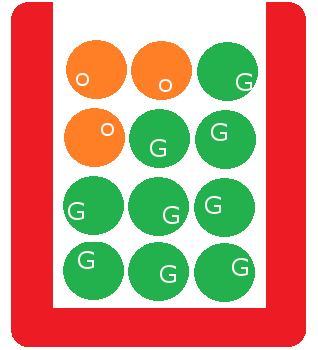
\includegraphics[width=2in]{02Background/prob/RedUrnMarked.png}
	\end{center}
	\caption[ตัวอย่างความน่าจะเป็น ลังใส่ลูกบอล]{ลังใส่ลูกบอล ซึ่งมีลูกบอลอยู่ภายใน $12$ ลูก เป็นลูกบอลสีส้มสามลูก และที่เหลือเป็นสีเขียว}
	\label{fig: prob red box}
\end{figure}
%

%
\begin{figure}
	\begin{center}
		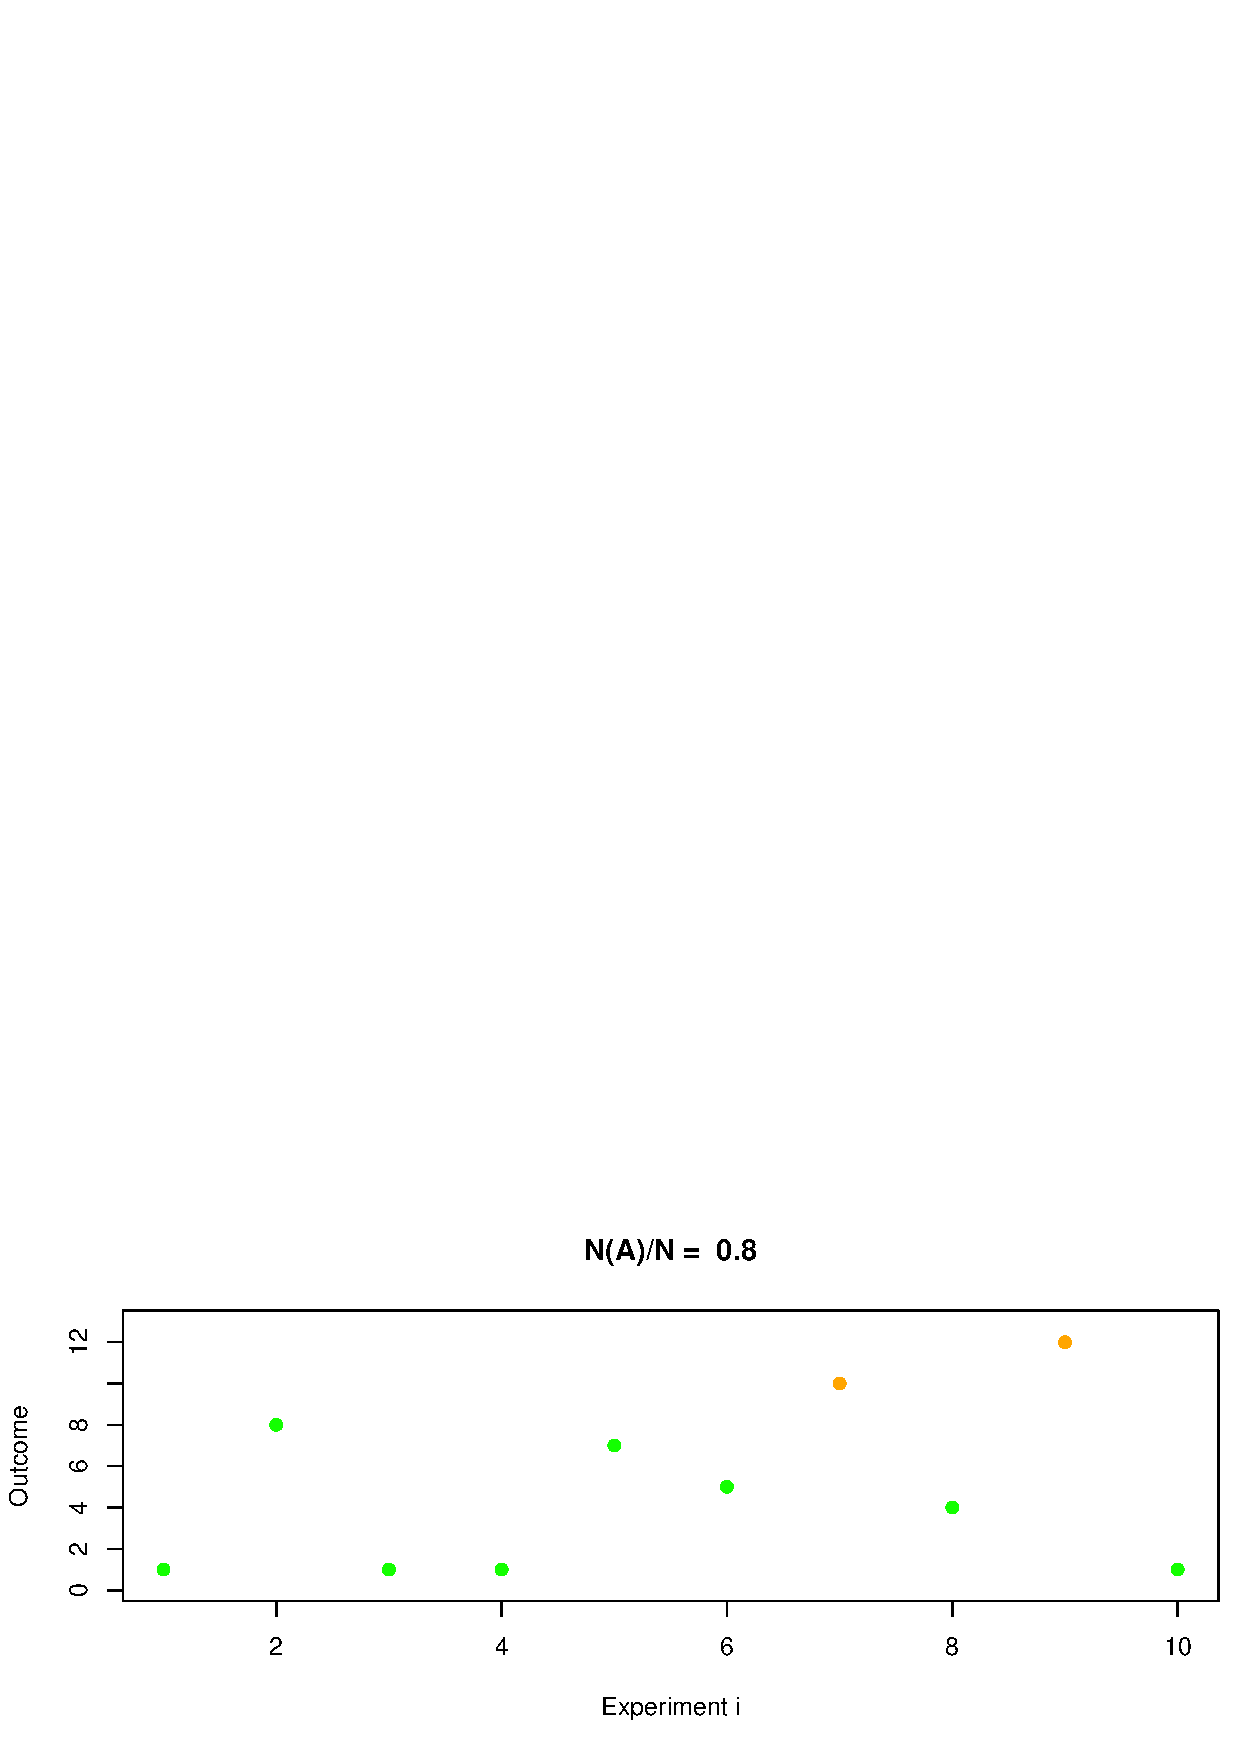
\includegraphics[width=4in]{02Background/prob/probDemo01.png}
	\end{center}
	\caption[ผลจากจำลองสุ่มหยิบลูกบอล]{ผลจากจำลองเหตุการณ์สุ่มหยิบลูกบอล $10$ ครั้ง จากกล่องลูกบอลที่แสดงในรูป~\ref{fig: prob red box}.
		%  ในกล่องมีลูกบอล $12$ ลูก,
		ลูกที่ 1--9 สีเขียว ลูกที่ 10--12 สีส้ม.
		จากการสุ่มทำ $10$ ครั้ง มีครั้งที่ 7 และ 9 ที่หยิบได้ลูกบอลสีส้ม.
		ดังนั้น อัตราส่วนจำนวนครั้งที่หยิบได้ลูกบอลสีเขียว คือ $0.8$ (ระบุที่ด้านบนของภาพ)}
	\label{fig: prob red box result N 10}
\end{figure}
%

\begin{table}[hbtp]
%	{\scriptsize
		\caption[อัตราส่วนของการหยิบได้สีเขียว]{อัตราส่วนของการสุ่มได้ลูกบอลสีเขียว เมื่อจำนวนการทำซ้ำเพิ่มขึ้น}
		\begin{center}
			\begin{tabular}{|r|c|c|c|c|c|c|c|}
				\hline 
				$N$ & $10$ & $100$ & $1000$ & $10^4$ & $10^5$ & $10^6$ & $10^7$ \\
				\hline 
				$\frac{N(A)}{N}$ &
				$0.8$  & $0.68$  & $0.754$  & $0.7564$ & $0.74917$ & $0.749291$ &  $0.7499472$ \\
				\hline
			\end{tabular} 
		\end{center}
		\label{tbl: prob demo N(A)/N}
%	}%end \small
\end{table}

%
\begin{figure}
	\begin{center}
		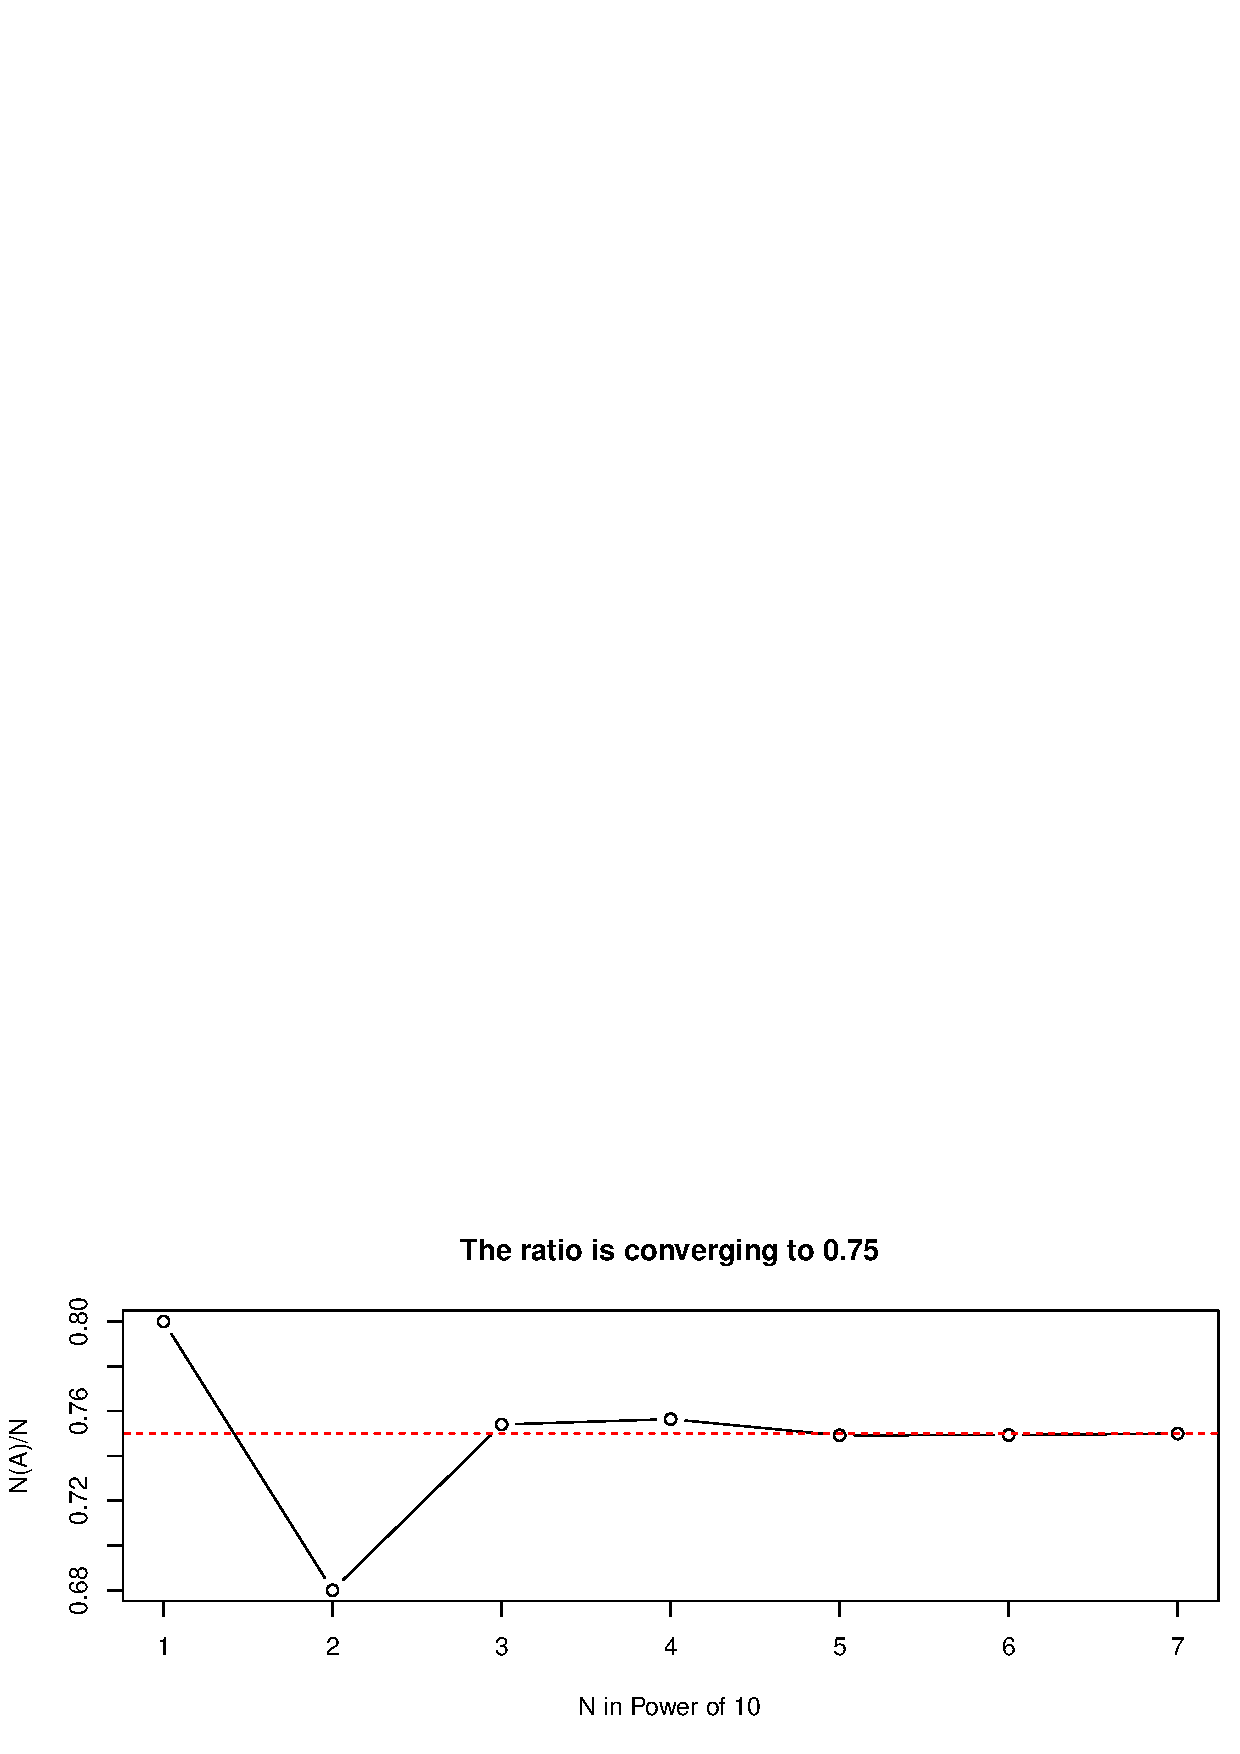
\includegraphics[width=4in]{02Background/prob/demoProb02.png}
	\end{center}
	\caption[การลู่เข้าของอัตราส่วนการหยิบได้สีเขียว]{อัตราส่วน $\frac{N(A)}{N}$ ลู่เข้าหา $\mathrm{Pr}(A) = 0.75$ เมื่อ $N$ เพิ่มขึ้น (แสดงด้วยเส้นประสีแดง)}
	\label{fig: prob demo N(A)/N}
\end{figure}
%

%
\begin{figure}
	\begin{center}
		
		\begin{tabular}{cc}
			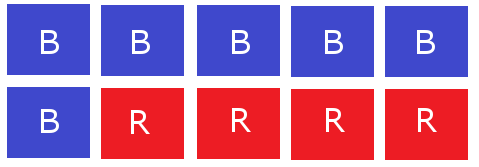
\includegraphics[width=2in]{02Background/prob/boxesMarked.png}
			&
			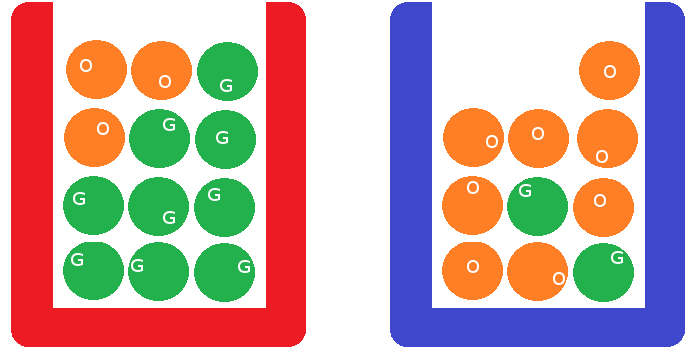
\includegraphics[width=2in]{02Background/prob/TwoUrnsMarked.png}
			\\
			(a) & (b) \\
		\end{tabular} 
	\end{center}
	\caption[ตัวอย่างความน่าจะเป็นแบบมีเงื่อนไข]{ตัวอย่างลังบรรจุลูกบอลสี.
		ภาพ (a) แสดงจำนวนลังสีฟ้ากับลังสีแดง (มีลังสีแดงอยู่ $4$ ลัง ที่เหลือเป็นสีฟ้า).
		ภาพ (b) แสดงลูกบอลสีภายในลัง โดย
		ลังซ้ายสีแดงมีลูกบอลสีส้มอยู่ $3$ ลูก ที่เหลือสีเขียว
		และลังขวาสีฟ้ามีลูกบอลสีเขียวอยู่ $2$ ลูก ที่เหลือสีส้ม}
	\label{fig: prob boxes}
\end{figure}
%

\paragraph{คุณสมบัติของความน่าจะเป็น.}
ความน่าจะเป็นมีคุณสมบัติที่น่าสนใจหลายอย่าง
เช่น
ความน่าจะเป็นที่จะเกิดผลลัพธ์จากกลุ่มผลลัพธ์ทั้งหมดทุกแบบที่เป็นไปได้ คือ ต้องพบแน่นอน ความน่าจะเป็นมีค่าสูงสุด.
นั่นคือ
$\mathrm{Pr}(\Omega) = 1$.
ความน่าจะเป็นที่จะพบเหตุการณ์ที่เป็นไปไม่ได้ คือ ต้องไม่พบแน่นอน ความน่าจะเป็นมีค่าต่ำสุด.
นั่นคือ
$\mathrm{Pr}(\emptyset) = 0$.
สัมพันธ์ด้านความน่าจะเป็นของเหตุการณ์ $A$ 
กับ $A^c$ คือ
$\mathrm{Pr}(A) = 1 - p(A^c)$
และ $\mathrm{Pr}(A \cup A^c) = 1$ 
และ $\mathrm{Pr}(A \cap A^c) = 0$.
ความน่าจะเป็นของยูเนียน คือ
$\mathrm{Pr}(A \cup B) = \mathrm{Pr}(A \setminus B) + \mathrm{Pr}(B \setminus A) + \mathrm{Pr}(A \cap B)$
หรือ
$\mathrm{Pr}(A \cup B) = \mathrm{Pr}(A) + \mathrm{Pr}(B) - \mathrm{Pr}(A \cap B)$.
ความน่าจะเป็นของผลต่าง คือ
$\mathrm{Pr}(A \setminus B) = \mathrm{Pr}(A) - \mathrm{Pr}(A \cap B)$.

\paragraph{เหตุการณ์ที่ไม่มีส่วนร่วมกัน.}
ถ้า $A \cap B = \emptyset$ 
แล้วจะเรียกว่า เหตุการณ์ $A$ และเหตุการณ์ $B$ \textbf{ไม่มีส่วนร่วมกัน} (disjoint)
\index{english}{probability!disjoint}
\index{thai}{ความน่าจะเป็น!ไม่มีส่วนร่วมกัน}
และยูเนียนของเหตุการณ์ที่ไม่มีส่วนร่วมกัน จะมีความน่าจะเป็น $\mathrm{Pr}(A \cup B) = \mathrm{Pr}(A) + \mathrm{Pr}(B)$.

\paragraph{กฎของการรวมความน่าจะเป็น.}
ถ้า $B_1 \cup B_2 \cup \ldots \cup B_n = \Omega$
และ $B_i \cap B_j = \emptyset$ สำหรับทุกๆค่าของ $i \neq j$ ตั้งแต่ $1, \ldots, n$
แล้ว
\textbf{กฎของความน่าจะเป็นรวม} (law of total probability)
\index{english}{probability!sum rule}
\index{english}{law of total probability}
\index{thai}{กฎของความน่าจะเป็นรวม}
กล่าวว่า
\begin{eqnarray}
\mathrm{Pr}(A) = \sum_{i=1}^n \mathrm{Pr}(A \cap B_i)
\label{eq: prob law of total prob}
\end{eqnarray}
จาก\textit{กฎของความน่าจะเป็นรวม}
กรณีพิเศษ คือ $\mathrm{Pr}(A) = \mathrm{Pr}(A \cap B) + \mathrm{Pr}(A \cap B^c)$.

\paragraph{ตัวแปรสุ่ม.}
\index{thai}{ตัวแปรสุ่ม}
\index{english}{random variable}
เพื่อความสะดวก
เหตุการณ์อาจถูกระบุด้วย
\textit{ตัวแปรสุ่ม} 
เช่น จากตัวอย่าง
เหตุการณ์ที่หยิบได้ลูกบอลสีเขียว
และเหตุการณ์ที่หยิบได้ลูกบอลสีส้ม
จะสามารถถูกอ้างถึงได้สะดวก และชัดเจนกว่า
ถ้ากำหนด \textit{ตัวแปรสุ่ม} $B$ แทนสีของลูกบอลที่ถูกสุ่มหยิบขึ้นมา.
เหตุการณ์ที่หยิบได้ลูกบอลสีเขียว 
สามารถ เขียนเป็น $B = 0$
เมื่อ $0$ แทนสีเขียว %\mbox{`g'}$
และ 
เหตุการณ์ที่หยิบได้ลูกบอลสีส้ม 
สามารถ เขียนเป็น $B = 1$
เมื่อ $1$ แทนสีส้ม.
\textbf{ตัวแปรสุ่ม} (random variable)
อาจถูกนิยามว่า
เป็นตัวแปรที่ค่าของมันขึ้นกับผลลัพธ์ของเรื่องที่สนใจ เมื่อเรื่องที่สนใจเป็นกระบวนการที่มี\textit{ความไม่แน่นอน}อยู่.
%a variable whose values depend on outcomes of a random phenomenon

หมายเหตุ \textit{ตัวแปรสุ่ม}เป็นการแทน\textit{เหตุการณ์}ด้วยค่าตัวเลข
โดยสำหรับธรรมชาติของเหตุการณ์ที่ไม่ได้เป็นตัวเลข การใช้งานตัวแปรสุ่มนี้อาจทำได้โดยการกำหนดความหมายให้กับตัวเลข 
เช่น $0$ แทนสีเขียว และ $1$ แทนสีส้ม.
แต่หลาย ๆ ครั้งเพื่อความสะดวกและชัดเจน
อาจมีการใช้สัญลักษณ์ เช่น
$\mbox{`g'}$ แทนตัวเลข $0$ ในกรณีที่ระบุถึงสีเขียว.

\textbf{ฟังก์ชันการแจกแจง} (distribution function)
	\index{thai}{ฟังก์ชันการแจกแจง}
	\index{english}{distribution function}
	ของ\textit{ตัวแปรสุ่ม} $X$
คือฟังก์ชัน 
$F: \mathbb{R} \rightarrow [0,1]$ 
โดย
$F(x) = \mathrm{Pr}(X \leq x)$.

ตัวแปรสุ่มอาจมีได้หลายแบบขึ้นกับลักษณะของค่าของมัน ซึ่งค่าของมันก็คือลักษณะของผลลัพธ์ที่เป็นไปได้.
\textbf{ตัวแปรสุ่มวิยุต} (discrete random variable)
คือตัวแปรสุ่มที่ค่าของมัน อยู่ใน\textit{เซตจำกัด} (finite set) หรืออยู่ใน\textit{เซตไม่จำกัดแต่นับได้} (countably infinite set).
ตัวอย่าง \textit{ตัวแปรสุ่ม}สีของลูกบอล $B$ นี้เป็น\textit{ตัวแปรสุ่มวิยุต}
เนื่องจากค่าของมันมาจาก\textit{เซตจำกัด} ได้แก่ $\{0, 1\}$ (มีจำนวนสมาชิกน้อยกว่าค่าอนันต์ $\infty$).
\textit{ตัวแปรสุ่ม}จำนวนต้นทุเรียน ก็เป็น\textit{ตัวแปรสุ่มวิยุต}
เนื่องจากค่าของมันมาจาก\textit{เซตไม่จำกัดแต่นับได้} ได้แก่ $\{0, 1, 2, 3, \ldots \}$.
แต่\textit{ตัวแปรสุ่ม}ปริมาณน้ำในอ่างเก็บน้ำ ไม่ใช่\textit{ตัวแปรสุ่มวิยุต}
เพราะว่า ค่าของมันมาจาก $\mathbb{R}^+$ 
%เช่น ปริมาณน้ำปีนี้อาจจะน้อยเหลือแค่ $8203046.91$ ลบ.ม.
\textit{ตัวแปรสุ่ม}ปริมาณน้ำในอ่างเก็บน้ำ จะเป็น\textit{ตัวแปรสุ่มต่อเนื่อง}.
หัวข้อ~\ref{sec: continuous random variable} อภิปราย\textit{ตัวแปรสุ่มต่อเนื่อง}เพิ่มเติม.

\textit{ตัวแปรสุ่มวิยุต} $X$ จะมี\textbf{ฟังก์ชันมวลความน่าจะเป็น} (probability mass function คำย่อ pmf) $f: \mathbb{R} \rightarrow [0,1]$ โดย $f(x) = \mathrm{Pr}(X = x)$.
\index{english}{probability mass function}
\index{english}{probability!mass function}
\index{english}{pmf}
\index{thai}{ฟังก์ชันมวลความน่าจะเป็น}


%\paragraph{ค่าคาดหมาย.}
\textbf{ค่าคาดหมาย} (expectation หรือ expected value) 
\index{english}{expectation}
\index{english}{expected value}
\index{thai}{ค่าคาดหมาย}
เป็น\textit{ค่าเฉลี่ย}ของ\textit{ตัวแปรสุ่ม}
และใช้สัญกรณ์ เช่น $E[X]$
สำหรับค่าคาดหมายของตัวแปรสุ่ม $X$.
โดยสำหรับ\textit{ตัวแปรสุ่มวิยุต}ที่เป็นตัวเลข
\textit{ค่าคาดหมาย}สามารถคำนวณได้จาก
\begin{eqnarray}
E[X] &=& \sum_x x \cdot \mathrm{Pr}(X=x)
\label{eq: prob expectation}.
\end{eqnarray}


\textbf{ความแปรปรวน} (variance)
\index{thai}{ความแปรปรวน}
\index{english}{variance}
ของ\textit{ตัวแปรสุ่ม}
ใช้สัญกรณ์ เช่น
$\mathrm{var}[X]$
ซึ่งค่า\textit{ความแปรปรวน} คำนวณได้จาก
\begin{eqnarray}
\mathrm{var}[X] &=& 
E[(X -E[X])^2]
\label{eq: prob variance}
\end{eqnarray}

% LATER
% ตัวอย่าง

\paragraph{ความน่าจะเป็นร่วม.}
\index{thai}{ความน่าจะเป็นร่วม}
\index{english}{joint probability}
\index{english}{probability!joint}
เมื่อใช้\textit{ตัวแปรสุ่ม}อธิบายเหตุการณ์
ในกรณีที่สนใจเหตุการณ์ที่เกี่ยวข้องกับ\textit{ตัวแปรสุ่ม}ตั้งแต่สองตัวขึ้นไป 
ความน่าจะเป็นที่ใช้ จะเรียกว่า
\textbf{ความน่าจะเป็นร่วม} (joint probability)
และใช้สัญกรณ์ 
เช่น $\mathrm{Pr}(X, Y)$ หรือ\textbf{ความน่าจะเป็นร่วม}ของ\textit{ตัวแปรสุ่ม} $X$ และ\textit{ตัวแปรสุ่ม} $Y$
และ\textit{ความน่าจะเป็นร่วม}
$\mathrm{Pr}(X, Y) = \mathrm{Pr}(X \cap Y)$.
นั่นคือ
$\mathrm{Pr}(X = x, Y = y)$
หมายถึง
ความน่าจะเป็นที่
\textit{ตัวแปรสุ่ม} $X$ จะมีค่าเป็น $x$
และ\textit{ตัวแปรสุ่ม} $Y$ จะมีค่าเป็น $y$.
%(หมายเหตุ สัญกรณ์ เช่น $\mathrm{Pr}(X, Y)$ เป็นการระบุถึง\textit{ความน่าจะเป็นร่วม}
%ในลักษณะทั่วไป และมักจะใช้เมื่อพิจารณรูปสมการที่แสดงความสัมพันธ์ระหว่างค่าตัวแปรสุ่มและค่าความน่าจะเป็น.)
%= placeholder

\textbf{ความแปรปรวนร่วมเกี่ยว} (covariance)
\index{thai}{ความแปรปรวนร่วมเกี่ยว}
\index{english}{covariance}
ของ\textit{ตัวแปรสุ่ม}สองตัว
ใช้สัญกรณ์ เช่น
$\mathrm{cov}[X, Y]$
ซึ่งค่า\textit{ความแปรปรวนร่วมเกี่ยว} คำนวณได้จาก
\begin{eqnarray}
\mathrm{cov}[X, Y] &=& 
E_{X,Y}[(X - E[X])(Y - E[Y])]
\nonumber \\
&=& E_{X,Y}[XY] - E[X]E[Y]
\label{eq: prob covariance}
\end{eqnarray}
เมื่อ $E_{X,Y}$ หมายถึง\textit{ค่าคาดหมาย} ที่คิดโดยคำนึงถึงความน่าจะเป็นร่วมของ $X$ และ $Y$.
นั่นคือ
สำหรับตัวแปรสุ่มวิยุต
$ 
\mathrm{cov}[X, Y] =
\sum_x \sum_y (x - E[X])(y - E[Y]) \cdot \mathrm{Pr}(X=x, Y=y)$.


\subsection{ความน่าจะเป็นแบบมีเงื่อนไข} 
\label{sec: cond prob}
\index{english}{conditional probability}
\index{thai}{ความน่าจะเป็นแบบมีเงื่อนไข}
\index{english}{probability!conditional}
\index{thai}{ความน่าจะเป็น!แบบมีเงื่อนไข}

\textbf{ความน่าจะเป็นแบบมีเงื่อนไข} (conditional probability) 
ประมาณโอกาสที่จะเกิดเหตุการณ์ที่สนใจ ในกรณีที่รู้ผลลัพธ์ของเงื่อนไข.
\textit{ความน่าจะเป็นแบบมีเงื่อนไข}จะเน้นบริบทของเงื่อนไข.
สัญกรณ์ เช่น $\mathrm{Pr}(A|B)$ 
แทน\textit{ความน่าจะเป็นแบบมีเงื่อนไข} 
ที่หมายถึง \textit{ความน่าจะเป็น}ของเหตุการณ์ $A$
ในกรณีที่เหตุการณ์ $B$ เป็นจริง.
เหตุการณ์ $B$ เป็นเงื่อนไข
และเป็นบริบทเสริม เป็นข้อมูลเสริมในการประมาณความน่าจะเป็น.

จากตัวอย่างของรูป~\ref{fig: prob red box} 
พิจารณาตัวอย่างที่คราวนี้
มีลังอยู่ $10$ ลัง ซึ่ง เป็นลังสีแดง $4$ ลัง และเป็นลังสีบานเย็น $6$ ลัง ดังรูป~\ref{fig: prob boxes}.
ถ้าสุ่มยกมาหนึ่งลัง โอกาสที่จะเป็นลังที่ 7 คือ $1/10$
แต่ถ้าเห็นว่าลังที่สุ่มมาเป็นสีแดง โอกาสที่จะเป็นลังที่ 7 คือ $1/4$ เพราะว่า มีแค่ลังที่ 7 ถึงลังที่ 10 ที่เป็นสีแดงอยู่แค่ $4$ ลัง.
ถ้าเห็นว่าลังที่สุ่มมาสีบานเย็น โอกาสที่จะเป็นลังที่ 7 ไม่มีเลย หรือโอกาสเป็น $0$ เพราะลังที่ 7 สีแดง.
ข้อมูลพิเศษ หรือบริบทเพิ่มเติมนี้ คือเงื่อนไขที่ใช้ประกอบการประมาณโอกาสของเหตุการณ์.


\paragraph{การคำนวณ.}
ความน่าจะเป็นแบบมีเงื่อนไข
สามารถคำนวณได้จาก
\begin{eqnarray}
\mathrm{Pr}(A|B) = \frac{\mathrm{Pr}(A \cap B)}{\mathrm{Pr}(B)}
\label{eq: prob cond prob relation}
\end{eqnarray}
เมื่อ $\mathrm{Pr}(B) > 0$.
จากสมการ~\ref{eq: prob cond prob relation} จะได้
\begin{eqnarray}
\mathrm{Pr}(X, Y) = \mathrm{Pr}(X|Y) \cdot \mathrm{Pr}(Y)
\label{eq: prob product rule}
\end{eqnarray}
เมื่อ $X$ และ $Y$ คือตัวแปรสุ่ม.
สมการ~\ref{eq: prob product rule} มักเรียกว่า \textbf{กฎผลคูณ} (product rule).
\index{english}{product rule}
\index{thai}{กฎผลคูณ}
นอกจากนั้น พิจารณาสมการ~\ref{eq: prob law of total prob} และ~\ref{eq: prob product rule}  จะพบว่า 
\begin{eqnarray}
\mathrm{Pr}(X) = \sum_y \mathrm{Pr}(X, Y=y) = \sum_y \mathrm{Pr}(X|Y = y) \cdot \mathrm{Pr}(Y = y) 
\label{eq: prob sum rule}
\end{eqnarray}
ซึ่ง สมการนี้มักเรียกว่า \textbf{กฎผลรวม} (sum rule).
\index{english}{sum rule}
\index{thai}{กฎผลรวม}
สังเกตว่า การใช้\textit{กฎผลรวม}
จะลดตัวแปรสุ่มลงไป
ซึ่งการทำเช่นนี้ 
จึงอาจถูกเรียกว่า \textit{การสลายปัจจัย} (marginalization).
\index{english}{marginalization}
\index{thai}{การสลายปัจจัย}



\textit{กฎผลคูณ}สามารถใช้ต่อเนื่องกัน ในลักษณะลูกโซ่
\begin{eqnarray}
\mathrm{Pr}(X_1, X_2, \ldots, X_n) 
&=& \mathrm{Pr}(X_1) \cdot \mathrm{Pr}(X_2, \ldots, X_n|X_1)
\nonumber \\
&=& \mathrm{Pr}(X_1) \cdot \mathrm{Pr}(X_2|X_1)
\cdot \mathrm{Pr}(X_3, \ldots, X_n|X_1, X_2)
\nonumber \\
&\vdots& 
\nonumber \\
&=& \mathrm{Pr}(X_1) \cdot \mathrm{Pr}(X_2|X_1)
\cdot \mathrm{Pr}(X_3|X_1, X_2)
\cdot \mathrm{Pr}(X_4|X_1, X_2, X_3)
\cdot \cdots
\nonumber \\
&\;& \;
\cdots \mathrm{Pr}(X_n|X_1, \ldots, X_{n-1})
\label{eq: prob chain rule}
\end{eqnarray}
ซึ่งสมการ~\ref{eq: prob chain rule} มักจะถูกเรียกว่า \textbf{กฎลูกโซ่ของความน่าจะเป็น} (chain rule of probability).
\index{thai}{กฎลูกโซ่ของความน่าจะเป็น}
\index{english}{chain rule of probability}

\textbf{กฎของเบส์} (Bayes' rule หรือ Bayes' theorem)
\index{thai}{กฎของเบส์}
\index{english}{Bayes' rule}
\index{english}{Bayes' theorem} 
คือ
\begin{eqnarray}
\mathrm{Pr}(Y|X) &=& \frac{\mathrm{Pr}(X|Y) \cdot \mathrm{Pr}(Y)}{\mathrm{Pr}(X)}
\label{eq: prob Bayes' 1} \\
&=&
\frac{\mathrm{Pr}(X|Y) \cdot \mathrm{Pr}(Y)}{\sum_y \mathrm{Pr}(X|Y=y) \cdot \mathrm{Pr}(Y=y)}
\label{eq: prob Bayes' 2}
\end{eqnarray}
จากความสัมพันธ์ที่ได้จาก\textit{กฎของเบส์}
การอนุมานค่าที่สนใจจากข้อมูล
มักจะเรียกชื่อพจน์ต่าง ๆ
ในสมการ~\ref{eq: prob Bayes' 1} เพื่อความสะดวก ดังนี้
ถ้ากำหนดให้ตัวแปรสุ่ม $Y$ แทนเป้าหมายของการอนุมาน
และตัวแปรสุ่ม $X$ แทนข้อมูลประกอบ
แล้ว
$\mathrm{Pr}(Y)$ จะเรียกว่า \textit{ความน่าจะเป็นก่อน}
(prior probability คำย่อ prior)
ซึ่งหมายถึง ก่อนการนำข้อมูลประกอบมาคิด
$\mathrm{Pr}(Y|X)$ จะเรียกว่า
\textit{ความน่าจะเป็นภายหลัง}
(posterior probability คำย่อ posterior)
ซึ่งหมายถึง ภายหลังการนำข้อมูลประกอบมาคิด
และ
หาก $\mathrm{Pr}(X|Y)$ เขียนอยู่ในรูปฟังก์ชัน $f(y) = \mathrm{Pr}(X|Y=y)$
ก็จะถูกเรียกว่า \textit{ฟังก์ชันควรจะเป็น} (likelihood function คำย่อ likelihood).
ดังนั้น จาก\textit{กฎของเบส์}
และชื่อพจน์ต่าง ๆ อาจสรุปความสัมพันธ์ได้เป็น
$\mathrm{posterior} \propto \mathrm{likelihood} \cdot \mathrm{prior}$.

\paragraph{ตัวอย่างการคำนวณ.}
กลับมาที่รูป~\ref{fig: prob boxes}
อีกครั้ง คราวนี้จะสุ่มเลือกลัง และพอได้ลังแล้วก็จะสุ่มหยิบลูกบอลออกมา.
โอกาสที่จะสุ่มได้ลังแดงเป็น $\frac{4}{10}$ หรือความน่าจะเป็นที่จะได้ลังสีแดง $\mathrm{Pr}(C = \mbox{`r'}) = 0.4$
โดย $C = \mbox{`r'}$ แทนเหตุการณ์ที่จะได้ลังสีแดง.
ในทำนองเดียวกัน ความน่าจะเป็นที่จะได้ลังสีบานเย็น $\mathrm{Pr}(C = \mbox{`m'}) = 0.6$.

ถ้ารู้ว่าเป็นลังสีแดง เมื่อสุ่มหยิบลูกบอลมา โอกาสที่จะหยิบได้ลูกบอลสีเขียว คือ $\frac{9}{12} = 0.75$ 
หรือเขียนเป็นสัญกรณ์ ได้ว่า
$\mathrm{Pr}(B = \mbox{`g'}|C = \mbox{`r'}) = 0.75$
โดย $B = \mbox{`g'}$ แทนเหตุการณ์ที่จะหยิบได้ลูกบอลสีเขียว.
ทำนองเดียวกัน ก็จะได้\textit{ความน่าจะเป็นแบบมีเงื่อนไข}อื่น ๆ ดังนี้
\begin{itemize}
	\item $\mathrm{Pr}(B = \mbox{`o'}|C = \mbox{`r'}) = 0.25$,
	\item $\mathrm{Pr}(B = \mbox{`g'}|C = \mbox{`m'}) = 0.20$, 
	\item $\mathrm{Pr}(B = \mbox{`o'}|C = \mbox{`m'}) = 0.80$.
	\hfill $\square$	
\end{itemize}

สังเกตว่า \textit{ความน่าจะเป็นที่จะหยิบได้ลูกบอลสีเขียวเมื่อรู้ว่าลังสีแดง} $\mathrm{Pr}(B = \mbox{`g'}|C = \mbox{`r'})$ ไม่เหมือนกับ\textit{ความน่าจะเป็นที่จะหยิบลูกบอลสีเขียวและสุ่มได้ลังสีแดง} $\mathrm{Pr}(B = \mbox{`g'}, C = \mbox{`r'})$.
สำหรับ
$\mathrm{Pr}(B = \mbox{`g'}|C = \mbox{`r'}) = 0.75$
นั้นไม่ต้องสนใจเลยว่าโอกาสที่จะได้ลังสีแดงเป็นเท่าไร.
ในขณะที่
$\mathrm{Pr}(B = \mbox{`g'}, C = \mbox{`r'})$ จะประกอบด้วยโอกาสที่จะได้ลังสีแดง $\mathrm{Pr}(C = \mbox{`r'}) = 0.4$ และโอกาสที่จะหยิบได้ลูกบอลสีเขียวจากลังนั้น $\mathrm{Pr}(B = \mbox{`g'}|C = \mbox{`r'}) = 0.75$
ซึ่งจาก\textit{กฎผลคูณ} (สมการ~\ref{eq: prob product rule})
จะได้
\begin{eqnarray}
\mathrm{Pr}(B = \mbox{`g'}, C = \mbox{`r'}) &=& \mathrm{Pr}(C = \mbox{`r'}) \cdot \mathrm{Pr}(B = \mbox{`g'}|C = \mbox{`r'})
\nonumber \\
&=& (0.4) \cdot (0.75) = 0.3
\nonumber .
\end{eqnarray}

ในทำนองเดียวกันก็จะได้ค่าความน่าจะเป็นต่าง ๆ
ดังแสดงในตาราง~\ref{tbl: prob cond prob table}.

ทบทวน (1) ผลรวมของความน่าจะเป็นของทุก ๆ เหตุการณ์เป็น $1$. 
นั่นคือ
\begin{eqnarray}
\mathrm{Pr}(\Omega) &=& \mathrm{Pr}(C = \mbox{`r'}, B = \mbox{`g'})
+ \mathrm{Pr}(C = \mbox{`r'}, B = \mbox{`o'})
\nonumber \\
&\;&  
+ \mathrm{Pr}(C = \mbox{`b'}, B = \mbox{`g'})
+ \mathbb{P}(C = \mbox{`b'}, B = \mbox{`o'})    
\nonumber \\
&=& 0.3 + 0.1 + 0.12 + 0.48 = 1
\nonumber .
\end{eqnarray}
ธรรมชาตินี้เป็นคุณสมบัติพื้นฐานของความน่าจะเป็น.
ทบทวน (2) ความน่าจะเป็นของเหตุการณ์ $X$ เท่ากับผลรวมของความน่าจะเป็นของเหตุการณ์ $X$ และ $Y$ สำหรับทุก ๆ ความเป็นไปได้ของ $Y$ 
ดังเช่น
\begin{eqnarray}
\mathrm{Pr}(C = \mbox{`r'}) &=& \mathrm{Pr}(C = \mbox{`r'}, B = \mbox{`g'}) + \mathrm{Pr}(C = \mbox{`r'}, B = \mbox{`o'})
\nonumber \\
&=& 0.3 + 0.1 = 0.4
\nonumber \\
\mathrm{Pr}(C = \mbox{`m'}) &=& \mathrm{Pr}(C = \mbox{`m'}, B = \mbox{`g'}) + \mathrm{Pr}(C = \mbox{`m'}, B = \mbox{`o'})
\nonumber \\
&=& 0.12 + 0.48 = 0.6
\nonumber .
\end{eqnarray}
ธรรมชาตินี้คือ\textit{กฎผลบวก} (สมการ~\ref{eq: prob sum rule}).

จาก\textit{กฎของการบวก}
จะได้ ความน่าจะเป็นที่จะหยิบได้ลูกบอลสีเขียว และสีส้ม (โดยไม่สนใจสีของลัง)
\begin{eqnarray}
\mathrm{Pr}(B = \mbox{`g'}) &=& \mathrm{Pr}(C = \mbox{`r'}, B = \mbox{`g'}) + \mathrm{Pr}(C = \mbox{`m'}, B = \mbox{`g'})
\nonumber \\
&=& 0.3 + 0.12 = 0.42
\nonumber \\
\mathrm{Pr}(B = \mbox{`o'}) &=& \mathrm{Pr}(C = \mbox{`r'}, B = \mbox{`o'}) + \mathrm{Pr}(C = \mbox{`m'}, B = \mbox{`o'})
\nonumber \\
&=& 0.1 + 0.48 = 0.58
\nonumber .
\end{eqnarray}
และความน่าจะเป็นของลังถ้าหากรู้สีของลูกบอลที่สุ่มหยิบออกมาหนึ่งลูก
\begin{eqnarray}
\mathrm{Pr}(C = \mbox{`r'}|B = \mbox{`g'}) &=& \frac{\mathrm{Pr}(B = \mbox{`g'}|C = \mbox{`r'})
	\cdot \mathrm{Pr}(C = `r')}{\mathrm{Pr}(B = \mbox{`g'})}
\nonumber \\
&=& \frac{(0.75) (0.4)}{0.42} = 0.71
\nonumber . 
\end{eqnarray}
\textit{ความน่าจะเป็นแบบมีเงื่อนไข} และ\textit{ทฤษฎีของเบส์}
ช่วยให้สามารถหาค่า\textit{ความน่าจะเป็น}ที่สนใจได้
จาก\textit{ค่าของความน่าจะเป็น}อื่นที่ประเมิน\textit{ความน่าจะเป็น}ได้ง่ายกว่า
เช่น
$\mathrm{Pr}(B|C)$ จะประเมินได้ง่าย 
เพราะว่า ลูกบอลอยู่ในลัง ดังนั้นจะนับได้ง่ายว่า ในลังแต่ละสี มีลูกบอลสีไหนจำนวนเท่าไร ต่อจำนวนลูกบอลทั้งหมดในลัง.
$\mathrm{Pr}(C)$ ก็ประเมินได้ง่าย 
แต่ $\mathrm{Pr}(C|B)$ ประเมินตรง ๆ ได้ยาก
เพราะลูกบอลแต่สีกระจายไปทุก ๆ ลัง.

\begin{table}[hbtp]
	%{\scriptsize
	\caption[สรุปค่าความน่าจะเป็นร่วม]{สรุปค่าความน่าจะเป็นของตัวอย่างการสุ่มลังและลูกบอล}
	\begin{center}
		\begin{tabular}{|c|l|l|}
			\hline 
			ลัง & \multicolumn{2}{c|}{ลูกบอล $B$ } \\
			\cline{2-3}
			$C$ & เขียว `g' & ส้ม `o' \\
			\hline
			แดง `r' & 0.3 & 0.1 \\
			\hline
			บานเย็น `m' & 0.12 & 0.48 \\
			\hline
		\end{tabular} 
	\end{center}
	\label{tbl: prob cond prob table}
	%}%end \small
\end{table}


\paragraph{การตีความและความสับสนที่พบได้บ่อย.}
เพื่อหาความน่าจะเป็นที่จะได้ลูกบอลสีเขียว
$\mathrm{Pr}(B = \mbox{`g'})$
บ่อยครั้งมักถูกคำนวณด้วย
$11/22 = 0.5$ 
ซึ่งได้จากการนับลูกบอลสีเขียว เทียบกับลูกบอลทั้งหมด.
กรณีนี้
ค่าที่ถูกต้อง $\mathrm{Pr}(B = \mbox{`g'}) = 0.42$ 
ไม่เท่ากับ 
$11/22 = 0.5$ 
ซึ่ง $11/22$ ได้จากการนับลูกบอล
โดยเสมือนว่าไม่มีลัง.
กรณีหลังนั้น คือสถานการณ์ที่เทลูกบอลทั้งหมดออกจากลัง และสุ่มหยิบลูกไหนก็ได้.
ในขณะที่ตัวอย่างนี้ ต้องเลือกลังก่อน
ถ้าเลือกลังแล้ว ต้องสุ่มหยิบลูกจากในลังที่เลือก.

สองกรณีนี้ จะเห็นต่างกันชัดเจนมาก 
ถ้าพิจารณากรณี เช่น
ตัวอย่างในรูป~\ref{fig:prob common confusion} 
มีลังสีเหลืองแค่ $1$ ลัง มีลังสีฟ้า $4$ ลัง
แต่ลังสีเหลืองมีลูกบอล $8$ ลูก ที่ทั้งหมดสีเขียว
และลังสีฟ้ามีลูกบอล $2$ ลูก
ที่ทั้งหมดสีส้ม.
เมื่อคิดความน่าจะเป็นแล้วจะพบว่า
กรณีนี้
ถ้าเทลูกบอลทั้งหมดออกจากลัง แล้วสุ่มหยิบโอกาสที่จะได้สีเขียวเป็น $8/16 = 1/2$
แต่ถ้าสุ่มเลือกลังก่อน ลังสีเหลืองมีโอกาสแค่ $1/5$
แล้วโอกาสได้ลูกบอลสีเขียวจากลังนี้เป็น $1$ 
ในขณะที่โอกาสที่จะได้ลังสีฟ้าเป็น $4/5$ แต่โอกาสได้ลูกบอลสีเขียวเป็น $0$
ดังนั้นโอกาสได้ลูกบอลสีเขียวจะเป็นแค่ $(1/5) \cdot 1 + (4/5) \cdot 0 = 1/5$.

%
\begin{figure}
	\begin{center}
		\includegraphics[width=\textwidth]
		{02Background/prob/CommonConfusion.png}
	\end{center}
	\caption[ตัวอย่างเพิ่มเติม ความน่าจะเป็นแบบมีเงื่อนไข]{ตัวอย่างเน้นความต่างระหว่างสุ่มเลือกลังแล้วสุ่มเลือกลูกบอล (ในภาพ) เปรียบเทียบกับเทลูกบอลทั้งหมดมารวมกัน แล้วสุ่มเลือกลูกบอล (ไม่มีภาพ)}
	\label{fig:prob common confusion}
\end{figure}
%

ภาพความเกี่ยวเนื่องของเหตุการณ์ และความน่าจะเป็นร่วม และความน่าจะเป็นแบบมีเงื่อนไข
แสดงในรูป~\ref{fig:prob conditional visualization} สำหรับสองเหตุการณ์
และรูป~\ref{fig:prob conditional 3-event visualization} สำหรับสามเหตุการณ์.

%
\begin{figure}
	\begin{center}
		\includegraphics[width=\textwidth]
		{02Background/prob/cond_set2.png}
	\end{center}
	\caption[ความเกี่ยวเนื่องของสองเหตุการณ์]{ภาพแสดงความเกี่ยวเนื่องของเหตุการณ์ ภาพ ก แสดงเหตุการณ์ $A$ ด้วยวงกลมซ้าย และเหตุการณ์ $B$ ด้วยวงกลมขวา พื้นที่ที่ทับซ้อนกันคือ เหตุการณ์ร่วม $A \cap B$
	พื้นที่ทั้งหมดในกรอบคือผลลัพธ์ทุก ๆ แบบที่เป็นไปได้ ($\Omega$ หรือปริภูมิตัวอย่าง).
	ภาพ ข ความน่าจะเป็น $\mathrm{Pr}(A \cap B)$ มองโอกาสเกิดเหตุการณ์ร่วม $A \cap B$ จากบริบทของทุก ๆ ผลลัพธ์ที่เป็นไปได้. ภาพ ค ความน่าจะเป็น $\mathrm{Pr}(A | B)$ มองโอกาสเกิดเหตุการณ์ร่วม $A \cap B$ จากบริบทของเหตุการณ์ $B$.
    ภาพ ง ความน่าจะเป็น $\mathrm{Pr}(B | A)$ มองโอกาสเกิดเหตุการณ์ร่วม $A \cap B$ จากบริบทของเหตุการณ์ $A$.}
	\label{fig:prob conditional visualization}
\end{figure}
%

%
\begin{figure}
	\begin{center}
		\includegraphics[width=\textwidth]
		{02Background/prob/cond_set3.png}
	\end{center}
	\caption[ความเกี่ยวเนื่องของสามเหตุการณ์]{ภาพแสดงความเกี่ยวเนื่องของเหตุการณ์สามเหตุการณ์ ภาพ ก แสดงเหตุการณ์ $A$ เหตุการณ์ $B$ เหตุการณ์ $C$ ด้วยวงกลม
	พื้นที่ที่ทับซ้อนกันแทนเหตุการณ์ร่วม ฉลาก เช่น \texttt{(A,B)} ระบุเหตุการณ์ร่วม $A \cap B$
	และ \texttt{(A,B,C)} ระบุเหตุการณ์ร่วม $A \cap B \cap C$.
	พื้นที่ทั้งหมดในกรอบคือผลลัพธ์ทุก ๆ  แบบที่เป็นไปได้ ($\Omega$).
	ภาพ ข ความน่าจะเป็น $\mathrm{Pr}(A \cap B \cap C)$ มองโอกาสเกิดเหตุการณ์ร่วม $A \cap B \cap C$ จากบริบทของทุก ๆ ผลลัพธ์ที่เป็นไปได้. ภาพ ค ความน่าจะเป็น $\mathrm{Pr}(A | B, C)$ มองโอกาสเกิดเหตุการณ์ร่วม $A \cap B \cap C$ จากบริบทของเหตุการณ์ร่วม $B \cap C$.
	ภาพ ง ความน่าจะเป็น $\mathrm{Pr}(A, B | C)$ มองโอกาสเกิดเหตุการณ์ร่วม $A \cap B \cap C$ จากบริบทของเหตุการณ์ $C$.}
	\label{fig:prob conditional 3-event visualization}
\end{figure}
%


\paragraph{ความเป็นอิสระต่อกัน.}
เหตุการณ์ $A$ และเหตุการณ์ $B$
จะ\textbf{เป็นอิสระ}ต่อกัน (independent)
ก็ต่อเมื่อ
$\mathrm{Pr}(A \cap B) = \mathrm{Pr}(A) \cdot \mathrm{Pr}(B)$.
ดังนั้น จาก\textit{กฎผลคูณ} $\mathrm{Pr}(A \cap B) = \mathrm{Pr}(A|B) \cdot \mathrm{Pr}(B)$
จะได้ว่า $\mathrm{Pr}(A|B) = \mathrm{Pr}(A)$ เมื่อ $A$ และ $B$ เป็นอิสระต่อกัน.
ความหมายก็คือ
ถ้าเหตุการณ์ $A$ และเหตุการณ์ $B$ เป็นอิสระต่อกันแล้ว การรู้หรือไม่รู้ข้อมูลของ $B$ ก็ไม่ได้เปลี่ยนการประมาณค่าของ $A$.

\subsubsection{ตัวอย่างการใช้งานความน่าจะป็นแบบมีเงื่อนไข}
\label{sec: prob cond prob examples}

\paragraph{ปัญหาการตรวจเต้านมด้วยภาพเอ็กซเรย์.}
สมมติว่า ผู้หญิงอายุสี่สิบปีคนหนึ่ง ไปทำ\textit{การตรวจเต้านมด้วยภาพเอ็กซเรย์} (mammogram)
แล้วผลตรวจเป็น\textit{บวก} (positive ซึ่งหมายถึง เครื่องตรวจบอกว่าเป็นมะเร็ง)
โอกาสที่ผู้หญิงคนนี้จะเป็นมะเร็งจริง ๆ เป็นเท่าไร

สมมติว่าข้อมูลประกอบ คือ
วิธีการตรวจเต้านมด้วยเอ็กซเรย์มี\textit{ค่าความไว} (sensitivity) ที่ $80\%$
ซึ่งหมายความว่า ถ้าคนที่เป็นมะเร็งไปทำการตรวจแล้ว
โอกาสที่จะได้ผลเป็นบวก คือ $0.8$.
นั่นคือ $\mathrm{Pr}(M = 1|C = 1) = 0.8$
เมื่อ $M = 1$ แทนผลตรวจเป็นบวก (ถ้า $M = 0$ คือผลตรวจเป็นลบ)
และ $C = 1$ แทนผู้รับการตรวจเป็นมะเร็งจริง ๆ 
(ถ้า $C = 0$ คือผู้รับการตรวจไม่ได้เป็นมะเร็ง).

ความเข้าใจผิดอย่างหนึ่งที่พบบ่อย
คือ การสรุปว่า ผู้หญิงคนนั้นมีโอกาสเป็นมะเร็ง $80\%$ ซึ่งผิด
เพราะการสรุปนี้ ไม่ได้คำนึงถึง\textit{ความน่าจะเป็นก่อน} นั่นคือ โอกาสที่ผู้หญิงอายุสี่สิบปี
จะเป็นมะเร็งเต้านม ซึ่งจากสถิติ%
\footnote{%
จากรายงาน
Breast Cancer Facts \& Figures 2019-2020
ของ American Cancer Society.
%
%\url{https://www.cancer.org/content/dam/cancer-org/research/cancer-facts-and-statistics/breast-cancer-facts-and-figures/breast-cancer-facts-and-figures-2019-2020.pdf} (สืบค้น 18 มค 2563.
เนื้อหาของปัญหานี้ ดัดแปลงจาก \cite{Murphy2012}
โดยปรับปรุงสถิตินี้เป็นค่าล่าสุด.
}
คือ $17\%$.
นั่นคือ $\mathrm{Pr}(C = 1) = 0.17$.

นอกจากนั้น การสรุปยังต้องการข้อมูลว่า
วิธีการตรวจมี\textit{ผลบวกผิด} (false positive หรือสัญญาณหลอก false alarm)
\index{thai}{ผลบวกผิด} 
\index{english}{false positive}
เป็นเท่าไร
ถ้าวิธีการตรวจมี\textit{ผลบวกผิด} เป็น $10\%$.
นั่นคือ
$\mathrm{Pr}(M = 1|C = 0) = 0.1$.

ดังนั้น เมื่อรวมหลักฐานทุกอย่างเข้าด้วยกัน 
โดยใช้\textit{กฎของเบส์} จะได้ว่า
\begin{eqnarray}
\mathrm{Pr}(C = 1|M = 1) &=& \frac{\mathrm{Pr}(M = 1|C = 1) \mathrm{Pr}(C = 1)}{\mathrm{Pr}(M = 1|C = 0) \mathrm{Pr}(C = 0) + \mathrm{Pr}(M = 1|C = 1) \mathrm{Pr}(C = 1)}
\nonumber \\
&=& \frac{0.8 \cdot 0.17}{0.1 \cdot 0.83 + 0.8 \cdot 0.17}
= 0.62
\nonumber .
\end{eqnarray}
ดังนั้นคำตอบที่ถูกคือ $62\%$.

\paragraph{ปัญหามอนตี้ฮอล.}
ปัญหามอนตี้ฮอล (Monty Hall Problem)
\index{thai}{ปัญหามอนตี้ฮอล} \
\index{english}{Monty Hall Problem}
เป็นสถานการณ์การตัดสินใจของผู้เข้าแข่งขันเกมส์โชว์มอนตี้ฮอล. 
ผู้เข้าแข่งขันต้องเลือกเปิดประตูหนึ่งในสามประตู.
มีประตูหนึ่งที่ซ่อนรางวัลใหญ่ไว้.
อีกสองประตูมีแต่ของปลอบใจ.
ผู้เข้าแข่งขันจะได้อะไรก็ตามที่อยู่หลังประตูกลับบ้าน.
แต่หลังจากผู้เข้าแข่งขันเลือกประตูไปแล้ว แทนที่พิธีกรจะเปิดประตูนั้นออกทันที.
พิธีกรจะเดินไปที่ประตู
และเลือกเปิดประตูหนึ่ง ที่ผู้เข้าแข่งขันไม่ได้เลือก.
ประตูที่พิธีกรเปิด จะไม่มีรางวัลอยู่
และเสนอโอกาสให้ผู้เข้าแข่งขันเปลี่ยนใจ
ไปเลือกประตูที่เหลืออยู่.
ผู้เข้าแข่งขันควรจะเลือกยืนยันประตูเก่า หรือควรจะเลือกเปลี่ยนไปประตูใหม่

ปัญหานี้ ในมุมมองของ\textit{ความน่าจะเป็นแบบมีเงื่อนไข}
คือ การหาค่าความน่าจะเป็นที่ประตูใหม่จะมีรางวัล เปรียบเทียบกับการหาค่าความน่าจะเป็นที่ประตูเก่าจะมีรางวัล.

กำหนดให้
$\mathrm{Pr}(R = 3|C = 1, H = 2)$
แทน
การหาค่าความน่าจะเป็นที่รางวัลจะอยู่ประตูที่สาม
เมื่อผู้เข้าแข่งขันเลือกประตูที่หนึ่ง
และพิธีกรเปิดประตูที่สอง
โดย $R$ แทนประตูที่มีรางวัล
$C$ แทนประตูที่เลือก
และ $H$ แทนประตูที่พิธีกรเปิด.

พิจารณา กรณี
\begin{eqnarray}
\mathrm{Pr}(R = 1| C = 1, H = 2) &=& \frac{\mathrm{Pr}(R = 1, H = 2| C = 1)}{\mathrm{Pr}(H = 2| C = 1)}
\label{eq: prob monty hall stay}
\end{eqnarray}
ซึ่งเป็นตัวแทนของโอกาส 
ในกรณีผู้เข้าแข่งขันไม่เปลี่ยนใจแล้วได้รางวัล
เปรียบเทียบกับกรณี
\begin{eqnarray}
\mathrm{Pr}(R = 3| C = 1, H = 2) &=& \frac{\mathrm{Pr}(R = 3, H = 2| C = 1)}{\mathrm{Pr}(H = 2| C = 1)}
\label{eq: prob monty hall change}
\end{eqnarray}
ซึ่งเป็นตัวแทนของโอาส
ในกรณีผู้เข้าแข่งขันเปลี่ยนใจแล้วได้รางวัล.

เพื่อแก้สมการ~\ref{eq: prob monty hall stay}
และ~\ref{eq: prob monty hall change} 
\textit{กฎของเบส์}
ต้องการข้อมูลเพิ่มเติม.
โอกาสที่รางวัลจะอยู่ประตูไหน มีเท่า ๆ กัน.
นั่นคือ
$\mathrm{Pr}(R = 1) = \mathrm{Pr}(R = 2) = \mathrm{Pr}(R = 3) = 1/3$
และ เพราะประตูที่มีรางวัลเป็นอิสระกับประตูที่ผู้แข่งขันเลือก ดังนั้น $\mathrm{Pr}(R) = \mathrm{Pr}(R|C)$.
นั่นคือ
$\mathrm{Pr}(R = 1|C = 1) = \mathrm{Pr}(R = 2|C = 1) = \mathrm{Pr}(R = 3|C = 1) = 1/3$.

แต่พิธีกรต้องไม่เปิดประตูที่ผู้แข่งขันเลือก หรือไม่เปิดประตูที่มีรางวัล ดังนั้น
\\
\begin{tabular}{ll}
$\mathrm{Pr}(H = 2|C = 1, R = 1) = 1/2$ &
เพราะ พิธีกรเลือกเปิดประตูที่สองหรือที่สามก็ได้
\\
$\mathrm{Pr}(H = 2|C = 1, R = 2) = 0$ &
เพราะ พิธีกรเปิดประตูที่มีรางวัลไม่ได้
\\
$\mathrm{Pr}(H = 2|C = 1, R = 3) = 1$ &
เพราะ พิธีกรเปิดประตูที่สองได้เท่านั้น
\end{tabular}

จากข้อมูลประกอบเหล่านี้
อนุมานได้ว่า 
\begin{eqnarray}
\mathrm{Pr}(R = 1, H = 2| C = 1) 
&=& 
\mathrm{Pr}(H =2 | C = 1, R = 1) \cdot \mathrm{Pr}(R = 1| C= 1)
\nonumber \\
&=& (1/2) (1/3) = 1/6
\nonumber \\
\mathrm{Pr}(R = 2, H = 2| C = 1) 
&=& 
\mathrm{Pr}(H =2 | C = 1, R = 2) \cdot \mathrm{Pr}(R = 2| C= 1)
\nonumber \\
&=& (0) (1/3) = 0
\nonumber \\
\mathrm{Pr}(R = 3, H = 2| C = 1) 
&=& 
\mathrm{Pr}(H =2 | C = 1, R = 3) \cdot \mathrm{Pr}(R = 3| C= 1)
\nonumber \\
&=& (1) (1/3) = 1/3
\nonumber
\end{eqnarray}
ซึ่งเท่านี้ก็เพียงพอแล้ว จะสรุปได้ว่า
โอกาสที่จะได้รางวัล ถ้าผู้แข่งขันเปลี่ยนประตู จะมากกว่า โอกาสถ้าผู้แข่งขันไม่เปลี่ยน
(เพราะว่า
สมการ~\ref{eq: prob monty hall stay}
และ~\ref{eq: prob monty hall change}
มีตัวหารเท่ากัน).

อย่างไรก็ตาม ค่า $\mathrm{Pr}(H = 2|C = 1)$ ก็สามารถอนุมานได้จาก\textit{กฎผลรวม}.
นั่นคือ
\begin{eqnarray}
\mathrm{Pr}(H = 2|C = 1) 
&=& \mathrm{Pr}(R = 1, H = 2|C = 1) +
\mathrm{Pr}(R = 2, H = 2|C = 1) 
\nonumber \\
&\;& \quad
+
\mathrm{Pr}(R = 3, H = 2|C = 1)
\nonumber \\
&=& 1/6 + 0 + 1/3 = 3/6 = 1/2
\nonumber .
\end{eqnarray}
ดังนั้น สรุปได้ว่า
\\
\begin{tabular}{ll}
โอกาสเมื่อยืนยันประตูเดิม &
$\mathrm{Pr}(R = 1|C =1, H = 2) = (1/6)/(1/2) = 1/3$
\\
โอกาสเมื่อเปลี่ยนประตูใหม่ &
$\mathrm{Pr}(R = 3|C =1, H = 2) = (1/3)/(1/2) = 2/3$.
\end{tabular}

\subsection{ตัวแปรสุ่มต่อเนื่อง}
\label{sec: continuous random variable}
\index{english}{continuous random variable}
\index{thai}{ตัวแปรสุ่มต่อเนื่อง}
\textit{ตัวแปรสุ่ม} $X$ จะเรียกว่า
เป็น\textbf{ตัวแปรสุ่มต่อเนื่อง} (continuous random variable)
ก็ต่อเมื่อ
\textit{ฟังก์ชันการแจกแจง}
ที่อาจเรียก
\textbf{ฟังก์ชันการแจกแจงสะสม} (cumulative distribution function คำย่อ cdf)
\index{english}{cumulative distribution function}
\index{thai}{ฟังก์ชันการแจกแจงสะสม}
สามารถแสดงได้ในรูป
\begin{eqnarray}
F(x) = \int_{-\infty}^x f(u) du
\quad x \in \mathbb{R}
\label{eq: prob continuous rv}
\end{eqnarray}
สำหรับบาง\textit{ฟังก์ชันที่สามารถหาปริพันธ์ได้} (integrable function) $f: \mathbb{R} \rightarrow [0, \infty)$.
ฟังก์ชัน $f$ นี้จะเรียกว่า 
\textbf{ฟังก์ชันความหนาแน่นความน่าจะเป็น}
(probability density function บางครั้งอาจเรียก
\textit{ฟังก์ชันความหนาแน่น} density function คำย่อ pdf) ของ $X$.
%หรือ).

\paragraph{สิ่งที่มักสับสน.}
\textit{ตัวแปรสุ่มต่อเนื่อง}
มีีคุณสมบัติหลายอย่างที่มักถูกเข้าใจผิด.
ทั้ง\textit{ตัวแปรสุ่มวิยุต}และ\textit{ตัวแปรสุ่มต่อเนื่อง}ใช้บรรยายเหตุการณ์ ซึ่งเหตุการณ์จะสามารถนำไปหาค่า\textit{ความน่าจะเป็น}ได้.
\textit{ความน่าจะเป็น}
ยังมีคุณสมบัติเหมือนเดิม 
ไม่ว่า
จะเป็น
\textit{ความน่าจะเป็น}ของเหตุการณ์ที่บรรยายด้วย\textit{ตัวแปรสุ่มวิยุต}
หรือด้วย\textit{ตัวแปรสุ่มต่อเนื่อง}.
นั่นคือ
\textit{ความน่าจะเป็น}
มีค่าระหว่างศูนย์ถึงหนึ่ง 
และผลรวมของความน่าจะเป็นทั้งหมดเป็นหนึ่ง.

แต่\textit{ตัวแปรสุ่มวิยุต}และ\textit{ตัวแปรสุ่มต่อเนื่อง}มีคุณสมบัติหลาย ๆ อย่างต่างกัน.
กำหนดให้
$D$ เป็น\textit{ตัวแปรสุ่มวิยุต}
และ
$C$ เป็น\textit{ตัวแปรสุ่มต่อเนื่อง}
สำหรับ\textit{ตัวแปรสุ่มวิยุต}
ความน่าจะเป็นของแต่ละผลลัพธ์
คือค่า\textit{ฟังก์ชันมวลความน่าจะเป็น}ของค่าผลลัพธ์นั้น
นั่นคือ $\mathrm{Pr}(D = d) = \mathrm{pmf}(d)$.
แต่สำหรับ\textit{ตัวแปรสุ่มต่อเนื่อง}
ความน่าจะเป็นของแต่ละผลลัพธ์เป็นศูนย์เสมอ
ไม่ว่าค่านั้นจะเป็นเท่าไร
นั่นคือ $\mathrm{Pr}(C = c) = 0$.

แม้ว่า
\textit{ความน่าจะเป็น}ของแต่ละค่าเป็นศูนย์
แต่\textit{ความน่าจะเป็น}ของช่วงค่าสามารถหาได้.
วิธีประเมิน\textit{ความน่าจะเป็น} ในกรณี\textit{ตัวแปรสุ่มต่อเนื่อง}
จะใช้\textit{ฟังก์ชันการแจกแจง} $F(c) = \mathrm{Pr}(C \leq c)$
และ\textit{ความน่าจะเป็น} $\mathrm{Pr}(C > c) = 1 - F(c)$.
เมื่อต้องการประเมิน\textit{ความน่าจะเป็น}เป็นช่วง ก็สามารถทำได้โดย
$\mathrm{Pr}(c_0 < C \leq c_1) = F(c_1) - F(c_0)$.
หากต้องการประเมิน\textit{ความน่าจะเป็น}บริเวณรอบ ๆ ค่าใดก็สามารถทำได้โดย
$\mathrm{Pr}(c - \epsilon < C \leq c + \epsilon) = F(c + \epsilon) - F(c - \epsilon)$ เมื่อ $\epsilon$ ระบุระยะของบริเวณรอบ ๆ.
ข้อควรระวัง ถ้า $\epsilon$ เล็กมาก ๆ แล้ว $\mathrm{Pr}(c - \epsilon < C \leq c + \epsilon)$ จะใกล้กับศูนย์
(\textit{ความน่าจะเป็น}ของค่าจุดจุดหนึ่งของ\textit{ตัวแปรสุ่มต่อเนื่อง}เป็นศูนย์).
%สังเกตว่าขอบของช่วงค่า เมื่อพิจารณา\textit{ความน่าจะเป็น}ของ\textit{ตัวแปรสุ่มต่อเนื่อง} ไม่สำคัญ
%เพราะ\textit{ความน่าจะเป็น}ที่จุดใด ๆ เป็นศูนย์และทำให้ $\mathrm{Pr}(C < c) = \mathrm{Pr}(C \leq c)$.

\textit{ตัวแปรสุ่มวิยุต}มี $\mathrm{pmf}$ แต่ไม่มี $\mathrm{pdf}$.
\textit{ตัวแปรสุ่มต่อเนื่อง}มี $\mathrm{pdf}$ ไม่มี $\mathrm{pmf}$.
ค่าของ $\mathrm{pmf}(d) \in [0,1]$ สำหรับทุก ๆ ค่า $d$
เพราะว่าค่าของ $\mathrm{pmf}(d)$ คือค่าความน่าจะเป็น.
แต่ค่าของ $\mathrm{pdf}(c) \geq 0$ ซึ่งอาจจะใหญ่กว่า $1$ ได้.
อย่างไรก็ตาม 
\begin{eqnarray}
\int_{-\infty}^{\infty} \mathrm{pdf}(c) dc &=& F(\infty)
	= \mathrm{Pr}(C \leq \infty) = 1
\nonumber
\end{eqnarray}

ตาราง~\ref{tbl: prob continuous rv}
สรุปคุณสมบัติของ\textit{ตัวแปรสุ่มต่อเนื่อง}
ที่มักถูกเข้าใจผิด
เปรียบเทียบกับคุณสมบัติของ\textit{ตัวแปรสุ่มวิยุต}ในประเด็นเดียวกัน.

\begin{table}[hbtp]
%	{%\scriptsize
		\caption{คุณสมบัติที่มักสับสนของตัวแปรสุ่มต่อเนื่อง}
		\begin{center}
			\begin{tabular}{l|l|l}
				\hline
ประเด็น & ตัวแปรสุ่มวิยุต $D$ & ตัวแปรสุ่มต่อเนื่อง $C$
\\ \hline
ฟังก์ชัน & $\mathrm{pmf}$ & $\mathrm{pdf}$ 
\nonumber \\
ช่วงค่า  & $\mathrm{pmf}: \mathbb{R} \rightarrow [0, 1]$
& $\mathrm{pdf}: \mathbb{R} \rightarrow [0, \infty)$
\\
ความน่าจะเป็น & $\mathrm{Pr}(D = d) = \mathrm{pmf}(d)$			
& $\mathrm{Pr}(C = c) = 0$ \\	
& & $\mathrm{pdf}$ ไม่ใช่ค่าความน่าจะเป็น
\\
\hline
ฟังก์ชันการแจกแจง & $F(d) = \mathrm{Pr}(D \leq d)$ & $F(c) = \mathrm{Pr}(C \leq c)$
\\
& $F(d)= \sum_{u \leq d} \mathrm{pmf}(u)$
&
  $F(c)= \int_{-\infty}^c \mathrm{pdf}(u) du$
\\
\hline
ค่าคาดหมาย & $E[D] = \sum_d d \cdot \mathrm{pmf}(d)$
& $E[C] = \int_{-\infty}^{\infty} c \cdot \mathrm{pdf}(c) dc$
\\
\hline
%กฎผลรวม & $\mathrm{Pr}(D_1) = \sum_{d_2} \mathrm{pmf}(D_1, D_2 = d_2)$
%&
%$\mathrm{Pr}(C_1) = \int \mathrm{pdf}(C_1, C_2 = c_2) d c_2$
%\\
%\hline
			\end{tabular} 
		\end{center}
		\label{tbl: prob continuous rv}
%	}%end \small
\end{table}

% LATER 
% uniform distribution

\paragraph{การแจกแจงเกาส์เซียน.}
คุณสมบัติที่สำคัญของ\textit{ตัวแปรสุ่ม} $X$
ก็คือ
\textit{การแจกแจง} $F(x) = \mathrm{Pr}(X \leq x)$.
\textit{การแจกแจง}แบบต่อเนื่อง ชนิดหนึ่งที่สำคัญ คือ
\textbf{การแจกแจงเกาส์เซียน} (Gaussian distribution)
หรืออาจเรียกว่า 
\textbf{การแจกแจงปกติ} (normal distribution).
\index{english}{Gaussian distribution}
\index{english}{normal distribution}
\index{thai}{การแจกแจงเกาส์เซียน}
\index{thai}{การแจกแจงปกติ}
\index{english}{distribution!Gaussian}
\index{english}{distribution!normal}
\index{thai}{การแจกแจง!เกาส์เซียน}
\index{thai}{การแจกแจง!ปกติ}

\textit{การแจกแจงเกาส์เซียน} 
อธิบาย\textit{การแจกแจง}ของ\textit{ตัวแปรสุ่มต่อเนื่อง} $X$ ด้วย\textit{ฟังก์ชันความหนาแน่น}
\begin{eqnarray}
f(x) = \frac{1}{\sqrt{2 \pi \sigma^2}} \exp \left( - \frac{(x - \mu)^2}{2 \sigma^2} \right), \quad -\infty < x < \infty
\label{eq: prob gaussian pdf}
\end{eqnarray}
เมื่อ $\mu$ และ $\sigma^2$ เป็นพารามิเตอร์ของแบบจำลอง%
\footnote{%
ในที่นี้ 
\textit{การแจกแจงเกาส์เซียน} ถูกมองเป็นแบบจำลองที่ใช้ทำนายความน่าจะเป็นของ $X$.
}.
ฟังก์ชันการแจกแจงของ\textit{การแจกแจงเกาส์เซียน}
ไม่มี\textit{รูปแบบปิด} (closed form ซึ่งในคณิตศาสตร์ หมายถึง นิพจน์ที่สามารถเขียนโดยใช้การคำนวณพื้นฐานได้)
และ\textit{ฟังก์ชันการแจกแจง} มักเขียนในรูป
\begin{eqnarray}
F(x) = 
%\Phi \left(\frac{x - \mu}{\sigma} \right) = 
\frac{1}{2} \left( 1 + \mathrm{erf} \left(\frac{x - \mu}{\sigma \sqrt{2}} \right) \right)
\label{eq: prob gaussian cdf}
\end{eqnarray}
เมื่อ
\begin{eqnarray}
\mathrm{erf}(x) = \frac{2}{\sqrt{\pi}} \int_0^x \exp \left( -t^2 \right) dt
\label{eq: prob gaussian erf}.
\end{eqnarray}

รูป~\ref{fig: prob normal mu sigma} แสดงความสัมพันธ์ระหว่างพารามิเตอร์ $\mu$ กับ $\sigma$ 
และผลต่อค่า\textit{ความหนาแน่นความน่าจะเป็น}ของ\textit{การแจกแจงเกาส์เซียน}.
ค่า $\mu$ จะควบคุมตำแหน่งที่มีความหนาแน่นสูงสุด.
ค่า $\sigma$ ควบคุมการแผ่.
สังเกตว่า \textit{ความหนาแน่นความน่าจะเป็น} มีค่าเกินหนึ่งได้ (ภาพล่างที่สองจากซ้าย $\sigma = 0.2$).

รูป~\ref{fig: prob normal cdf} แสดง\textit{ความหนาแน่นความน่าจะเป็น} (pdf) และ\textit{การแจกแจงความน่าจะเป็น} (cdf).
สังเกตว่า \textit{การแจกแจงความน่าจะเป็น} 
จะเป็น\textit{ฟังก์ชันเพิ่ม} (increasing function)
เพราะว่า 
\textit{การแจกแจงความน่าจะเป็น} $F(x) = \mathrm{Pr}(X \leq x)$ 
ดังนั้น ที่ค่ามากขึ้น ความน่าจะเป็นจะไม่มีทางน้อยลง
และที่อนันต์ $F(\infty) = 1$.
\textit{การแจกแจงความน่าจะเป็น} 
เป็น\textit{ค่าปริพันธ์} (integral) ของ\textit{ความหนาแน่นความน่าจะเป็น}
ดังนั้น พื้นที่ใต้กราฟของ\textit{ความหนาแน่นความน่าจะเป็น} จนถึง ณ จุดที่สนใจ จะเท่ากับค่า\textit{การแจกแจงความน่าจะเป็น}.



%
\begin{figure}
	\begin{center}
		\includegraphics[width=\textwidth]
		{02Background/prob/gauss_pdf_mu_sigma.png}
	\end{center}
	\caption[การแจกแจงเกาส์เซียน]{ความหนาแน่นความน่าจะเป็น ของการแจกแจงเกาส์เซียน ที่ค่าพารามิเตอร์ต่าง ๆ.
	ภาพในแถวบน 
	แสดงผลของค่า $\mu$ ต่าง ๆ ตั้งแต่ $-1$ ถึง $2$   
	โดย ค่า $\mu$ ระบุอยู่ข้างบนแต่ละภาพ.
	ภาพซ้ายสุุด แสดงผลของค่า $\mu$ ต่าง ๆ ในภาพเดียวกัน เพื่อการเปรียบเทียบได้ชัดเจน. 
ภาพในแถวล่าง จัดเรียงในลักษณะเดียวกัน แต่เป็น
ผลของค่า $\sigma$ ต่าง ๆ ตั้งแต่ $0.2$ ถึง $2$.   
สังเกตว่า ความหนาแน่นความน่าจะเป็น มีค่ามากกว่าศูนย์เสมอ 
แต่อาจมีค่ามากกว่าหนึ่งได้ เช่นแสดงในภาพล่างที่สองจากซ้าย.
}
	\label{fig: prob normal mu sigma}
\end{figure}
%



%
\begin{figure}
	\begin{center}
		\begin{tabular}{cc}
		\includegraphics[width=0.4\columnwidth]
{02Background/prob/normal_pdf_cdf.png}
&
\includegraphics[width=0.4\columnwidth]
{02Background/prob/pdf_cdf_area.png}
\\
ก & ข
		\end{tabular}
	\end{center}

	\caption[ความหนาแน่นความน่าจะเป็นและการแจกแจงความน่าจะเป็นสะสม]{ภาพ ก แสดงความหนาแน่นความน่าจะเป็น (pdf) และการแจกแจงความน่าจะเป็นสะสม (cdf) ของการแจกแจงแบบเกาส์เซียน. 
	ภาพ ข แสดงค่าของการแจกแจงสะสม คือพื้นที่ใต้กราฟของความหนาแน่น. นั่นคือ ณ จุดที่แสดง $\mathrm{cdf}(x) = 0.95$ ซึ่งเท่ากับพื้นที่ใต้กราฟของความหนาแน่น (พื้นที่แรเงาสีเหลือง).}
	\label{fig: prob normal cdf}
\end{figure}
%


\section{การหาค่าดีที่สุด}
\label{sec: optimization}
\index{english}{optimization}
\index{english}{revise!optimization}
\index{thai}{การหาค่าดีที่สุด}
\index{thai}{ทบทวน!การหาค่าดีที่สุด}

\textit{การรู้จำรูปแบบ}
และ\textit{การเรียนรู้ของเครื่อง}
ถูกสร้างบนพื้นฐานของศาสตร์\textit{การหาค่าดีที่สุด}%
\footnote{%
เนื้อหาในหัวข้อนี้ได้รับอิทธิพลหลักจาก
\cite{ChongZak2ndEd}
และ \cite[App. B]{Eisenstein2019}
}
\textit{การรู้จำรูปแบบ} ต้องการค้นหารูปแบบที่สนใจออกมา
และต้องการให้ผลการค้นหานั้นผิดพลาดน้อยที่สุด.
\textit{การเรียนรู้ของเครื่อง} ต้องการที่จะทำภาระกิจที่ได้รับมอบหมาย ให้ได้สมรรถนะสูงสุด จากประสบการณ์ที่มี.

\textbf{การหาค่าดีที่สุด} (optimization) 
\index{thai}{การหาค่าดีที่สุด}
\index{english}{optimization}
คือ การหาค่าของปัจจัย (แทนด้วยตัวแปร)
ที่มีผลให้เป้าหมาย (แทนด้วยฟังก์ชันของตัวแปร)
มีค่าน้อยที่สุด (หรือมีค่ามากที่สุด ขึ้นกับเป้าหมายที่ต้องการ).
ปัจจัยที่ต้องการเลือก เรียกว่า \textbf{ตัวแปรตัดสินใจ} (decision variable)
และฟังก์ชันแทนเป้าหมาย ซึ่งประมาณความสัมพันธ์ระหว่างค่าของ\textit{ตัวแปรตัดสินใจ}และเป้าหมายที่ต้องการ เรียกว่า \textbf{ฟังก์ชันจุดประสงค์} (objective function). 
%หรืออาจเรียกง่าย ๆ ว่า \textbf{เป้าหมาย}.
\index{english}{decision variable}
\index{thai}{ตัวแปรตัดสินใจ}
\index{thai}{ฟังก์ชันจุดประสงค์}
\index{english}{objective function}
%

ตัวอย่าง ปัญหาการหาค่าดีที่สุด เช่น
การเลือกอุณหภูมิบ่มทุเรียน
และเป้าหมายคือได้ทุเรียนสุก ซึ่งวัดจากปริมาณน้ำตาล.
ถ้าปัจจัยค่าอุณหภูมิ แทนด้วยตัวแปร $x$  
และถ้ามีฟังก์ชัน $h$ ที่สามารถใช้ในการประมาณความสัมพันธ์
ระหว่างอุณหภูมิที่บ่มกับปริมาณน้ำตาลที่ได้
ดังนั้นตัวแปร $x$ คือ\textit{ตัวแปรตัดสินใจ}
และฟังก์ชัน $h$ คือ\textit{ฟังก์ชันจุดประสงค์}.
ถ้าปริมาณน้ำตาลที่ได้มาก เป็นดัชนีบอกว่าทุเรียนสุกดี
กรณีนี้คือ การหาค่า $x$ ที่ทำให้ได้ค่าฟังก์ชัน $h$ ที่มากที่สุด.

\paragraph{ปัญหาค่ามากที่สุด และปัญหาค่าน้อยที่สุด.}
การหาค่า\textit{ตัวแปรตัดสินใจ} ที่ทำให้ได้\textit{ฟังก์ชันจุดประสงค์}มีค่ามากที่สุด นั้นเรียกว่า \textbf{ปัญหาค่ามากที่สุด} (maximization problem).
\index{english}{maximization problem}
\index{english}{minimization problem}
\index{thai}{ปัญหาค่ามากที่สุด}
\index{thai}{ปัญหาค่าน้อยที่สุด}
ตัวอย่างปัญหาการเลือกอุณหภูมิบ่มทุเรียน
ข้างต้นเป็น \textit{การหาค่าดีที่สุด}แบบ\textit{ปัญหาค่ามากที่สุด}.
\textit{ปัญหาค่ามากที่สุด} ใช้สัญกรณ์ \begin{eqnarray}
\underset{x}{\mathrm{maximize}} & h(x)
\label{eq: opt max prob}
\end{eqnarray}
หรือ อาจเขียนย่อเป็น $\mathrm{max}_x \; h(x)$
ซึ่งระบุว่า ต้องการหาค่าของตัวแปรตัดสินใจ $x$ ที่ทำให้ฟังก์ชันจุดประสงค์ $h(x)$ มีค่ามากที่สุด.

ทำนองเดียวกัน 
การหาค่า\textit{ตัวแปรตัดสินใจ} ที่ทำให้ได้\textit{ฟังก์ชันจุดประสงค์}มีค่าน้อยที่สุด นั้นเรียกว่า \textbf{ปัญหาค่าน้อยที่สุด} (minimization problem).
ตัวอย่าง\textit{ปัญหาค่าน้อยที่สุด}
เช่น 
การหาเส้นทางขับรถจากขอนแก่นไปร้อยเอ็ด ที่ใช้เวลาเดินทางน้อยที่สุด (\textit{ตัวแปรตัดสินใจ}เลือกเส้นทาง และ\textit{ฟังก์ชันจุดประสงค์}ประมาณเวลาเดินทาง)
การหาทำเลตั้งเสาสัญญาณวิทยุ ที่ใช้งบประมาณรวมน้อยที่สุด
(\textit{ตัวแปรตัดสินใจ}เลือกตำแหน่งที่ตั้งเสาสัญญาณ และ\textit{ฟังก์ชันจุดประสงค์}ประเมินงบประมาณรวม)
การหารูปแบบการจัดรูปร่างของโปรตีน ที่ใช้พลังงานน้อยที่สุด
(\textit{ตัวแปรตัดสินใจ}เลือกรูปร่างของโปรตีน และ\textit{ฟังก์ชันจุดประสงค์}คำนวณพลังงานที่ใช้).
\textit{ปัญหาค่าน้อยที่สุด} ใช้สัญกรณ์ \begin{eqnarray}
\underset{x}{\mathrm{minimize}} & h(x)
\label{eq: opt min prob}
\end{eqnarray}
หรือ อาจเขียนย่อเป็น $\mathrm{min}_x \; h(x)$
ซึ่งระบุว่า ต้องการหาค่าของตัวแปรตัดสินใจ $x$ ที่ทำให้ฟังก์ชันจุดประสงค์ $h(x)$ มีค่าน้อยที่สุด.
บางครั้ง สัญกรณ์อาจระบุเซตของค่าตัวแปรตัดสินใจที่ใช้ค้นหา เช่น $\mathrm{min}_{x \in \mathbb{R}} \; h(x)$
ซึ่งระบุว่า ค่าของตัวแปรตัดสินใจสามารถเป็นจำนวนจริงใด ๆ
หรือ
$\mathrm{min}_{\bm{x} \in \mathbb{R}^2} \; h(\bm{x})$
ระบุว่า ค่าของตัวแปรตัดสินใจเป็นเวกเตอร์ที่มีสองส่วนประกอบจำนวนจริง.

ปัญหาค่าน้อยที่สุดและปัญหาค่ามากที่สุด จริง ๆ แล้ว
เป็นเสมือนเรื่องเดียวกันที่มองจากคนละมุม.
ปัญหาค่าน้อยที่สุดและปัญหาค่ามากที่สุด
สามารถแปลงไปมาระหว่างกันได้.
นั่นคือ
การหาตัวแปรตัดสินใจ $x$ ที่ทำให้ฟังก์ชันจุดประสงค์ $h(x)$ มีค่ามากที่สุด 
จะเทียบเท่ากับการหาค่า $x$ ที่ทำให้ $-h(x)$ มีค่าน้อยที่สุด.
นั่นคือ $\mathrm{max}_x \; h(x)$
$\equiv$
$\mathrm{min}_x \; -h(x)$.
%
รูป~\ref{fig: opt max min problems} 
แสดงภาพเปรียบเทียบค่าฟังก์ชัน $h(x)$ และ $-h(x)$ ที่เปรียบเสมือนภาพภูเขา และเงาของภาพภูเขาที่สะท้อนน้ำ โดยค่าของฟังก์ชันจะพลิกกลับรอบ ๆ ค่าศูนย์ (ค่าบวกเปลี่ยนเป็นลบ ค่าลบเปลี่ยนเป็นบวก ค่าศูนย์อยู่ที่เดิม ค่าบวกมากอยู่สูงจะเปลี่ยนเป็นค่าลบมากอยู่ต่ำ เป็นต้น).

ดังนั้นเพื่อความสะดวก ตำรานี้จะอ้างถึง \textit{ปัญหาค่าน้อยที่สุด} แทน\textit{ปัญหาการหาค่าดีที่สุด} โดยเฉพาะ เมื่ออภิปรายถึงวิธีการที่ใช้แก้ปัญหา
ซึ่งเมื่อปัญหาทั้งสองแบบเทียบเท่ากัน
วิธีต่าง ๆ ที่แก้\textit{ปัญหาค่าน้อยที่สุด}ได้
ก็สามารถใช้แก้\textit{ปัญหาค่ามากที่สุด}ได้เช่นกัน.

%ในบริบทของ\textit{ปัญหาค่าน้อยที่สุด}
หมายเหตุ
\textit{ฟังก์ชันจุดประสงค์} อาจถูกเรียกด้วยชื่ออื่น ๆ 
เช่น
ฟังก์ชันค่าใช้จ่าย (cost function),
ฟังก์ชันความสูญเสีย (loss function),
ฟังก์ชันพลังงาน (energy function),
ฟังก์ชันผลประโยชน์ (utility function) และ
ฟังก์ชันคุณค่า (value function).
ชื่อเหล่านี้ คือ\textit{ฟังก์ชันจุดประสงค์}.
แต่ชื่อของฟังก์ชันเหล่านี้
อาจบ่งบอกได้ชัดเจนกว่าว่า ปัญหาเป็นปัญหาค่าน้อยที่สุด 
(เช่น ฟังก์ชันค่าใช้จ่าย, 
ฟังก์ชันความสูญเสีย
และฟังก์ชันพลังงาน) 
หรือปัญหาเป็นปัญหาค่ามากที่สุด 
(เช่น ฟังก์ชันผลประโยชน์ และฟังก์ชันคุณค่า).
ชื่อเหล่านี้
มีการใช้อย่างกว้างขวางตามศาสตร์ ตามสาขาวิชา และตามงานประยุกต์ใช้งานด้านต่าง ๆ
เช่น
\textit{เศรษฐศาสตร์} มักใช้ฟังก์ชันผลประโยชน์,
ศาสตร์\textit{การวิจัยปฏิบัติการ} (operation research) มักพบคำว่า ฟังก์ชันค่าใช้จ่าย. 
ศาสตร์การเรียนรู้ของเครื่อง มักเลือกใช้คำว่า ฟังก์ชันความสูญเสีย.
ส่วนคำว่า ฟังก์ชันพลังงาน 
อาจพบเห็นได้บ้าง ในงานทางด้านการประมวลผลภาพ.
\index{english}{cost function}
\index{english}{loss function}
\index{english}{energy function}
\index{thai}{ฟังก์ชันค่าใช้จ่าย}
\index{thai}{ฟังก์ชันความสูญเสีย}
\index{thai}{ฟังก์ชันพลังงาน}

%
\begin{figure}
	\begin{center}
		\includegraphics[height=3.0in]
		{02Background/opt/minmax.png}
	\end{center}
	\caption[ปัญหาค่ามากที่สุดกับ ปัญหาค่าน้อยที่สุด]{ปัญหาค่ามากที่สุดกับ ปัญหาค่าน้อยที่สุดเป็นเรื่องเดียวกันที่มองจากคนละมุม. การหาค่า $x$ (เปรียบเหมือนตำแหน่งตามแนวนอน) ของ $h(x)$ ที่มากที่สุด (เปรียบเหมือนยอดเขา) เป็นเรื่องเดียวกับ การหาค่า $x$ ที่ทำให้ $-h(x)$ มีค่าน้อยที่สุด (ยอดเขาสูงเท่าไร เงาของยอดเขายิ่งต่ำลงมามากเท่านั้น แต่ตำแหน่งตามแนวนอนเป็นที่เดิม).}
	\label{fig: opt max min problems}
\end{figure}
%

ผลลัพธ์จาก\textit{การหาค่าดีที่สุด}
คือ 
ค่าของ\textit{ตัวแปรตัดสินใจ}
ที่ทำให้\textit{ฟังก์ชันจุดประสงค์}มีค่าน้อยที่สุด.
ค่าที่ได้นี้ เรียกว่า \textbf{ค่าทำให้น้อยที่สุด} (minimizer)
\index{english}{minimizer}
\index{thai}{ค่าทำให้น้อยที่สุด}
และนิยมใช้สัญลักษณ์เป็นตัวแปรตัดสินใจตามด้วยตัวยกที่เป็นดาว เช่น $x^\ast$ เพื่อระบุว่า กำลังกล่าวถึง \textit{ค่าทำให้น้อยที่สุด}ที่หามาเสร็จแล้ว ไม่ใช่ $x$ ที่เป็น \textit{ตัวแปรตัดสินใจ} ที่อาจใช้ค่าใด ๆ ก็ได้.
หมายเหตุ \textit{ค่าทำให้น้อยที่สุด} โดยทั่วไปจะไม่ใช่ค่าที่น้อยที่สุด.
รูป~\ref{fig: opt minimizers} แสดงแกนนอนแทนค่าของตัวแปรตัดสินใจ $x$ และแกนตั้งแทนค่าของฟังก์ชันจุดประสงค์ $f(x)$.
ค่า $x$ ที่น้อยที่สุด แทนด้วยสัญกรณ์ $x_{\min} $ คือ $-\infty$
เพราะว่า
$-\infty$ เป็นค่าที่น้อยที่สุดของจำนวนจริง และไม่ได้มีข้อจำกัดค่าของ $x$ (ดูหัวข้อ~\ref{sec: opt contrained opt} สำหรับกรณีปัญหาแบบมีข้อจำกัด).
ค่าทำให้น้อยที่สุด $x^\ast = x_1$ เพราะว่า
ที่ค่า $x_1$ ทำให้ฟังก์ชันจุดประสงค์มีค่าน้อยที่สุด นั่นคือ $f(x_1) = f_{\min}$
หรือ $f(x_1) \leq f(x)$ สำหรับทุก ๆ ค่าของ $x$.

สัญกรณ์ $\mathrm{min}_x \; f(x)$ นี้ใช้เพื่อระบุเป้าหมายและตัวแปรที่เกี่ยวข้องเท่านั้น.
หากต้องการระบุความสัมพันธ์ในสมการ
อาจใช้สัญกรณ์ เช่น $v = \arg\min_x f(x)$
เพื่อระบุว่า ค่า $v = x^\ast$  ที่หาได้จากการแก้ปัญหา $\min_x f(x)$.
หากต้องการระบุค่าฟังก์ชันจุดประสงค์ที่น้อยที่สุด
อาจระบุด้วยสัญกรณ์ เช่น $f(x^\ast)$ หรือ สัญลักษณ์ เช่น $f_{\min}$ เป็นต้น.

\paragraph{ค่าทำให้น้อยที่สุดท้องถิ่น และค่าทำให้น้อยที่สุดทั่วหมด.}
จากรูป~\ref{fig: opt minimizers}
สังเกตว่า แม้ $x_1$ จะเป็น\textit{ค่าทำให้น้อยที่สุด}
แต่ $x_2, x_3, x_4, x_5, x_6$ ก็มีลักษณะที่น่าสนใจ.
ค่า $x_1, x_2, x_3, x_4, x_5, x_6$ ทั้งหมด
จะเป็น \textit{ค่าทำให้น้อยที่สุดท้องถิ่น}.
\index{english}{local minimizer}
\index{english}{minimizer!local}
\index{thai}{ค่าทำให้น้อยที่สุดท้องถิ่น}
\index{thai}{ค่าทำให้น้อยที่สุด!ท้องถิ่น}
%
\textbf{ค่าทำให้น้อยที่สุดท้องถิ่น} (local minimizers)
คือ
ค่าของตัวแปรตัดสินใจ 
ที่ทำให้ฟังก์ชันจุดประสงค์มีค่าน้อยกว่าหรือเท่ากับค่าฟังก์ชันจุดประสงค์จากบริเวณรอบ ๆ.
กล่าวอีกอย่างได้ว่า
\textit{ค่าทำให้น้อยที่สุดท้องถิ่น} คือ ค่าที่ทำให้ฟังก์ชันจุดประสงค์มีค่าน้อยที่สุดในท้องถิ่น (ไม่มีใครในละแวกที่น้อยเกิน).
ค่า $x_1, x_2, x_3, x_4, x_5, x_6$ ต่างก็ทำให้ค่าฟังก์ชันจุดประสงค์น้อยกว่าหรือเท่ากับค่าจากบริเวณรอบ ๆ
แต่ค่า $x_1$ นอกจากจะทำให้ $f(x_1)$ มีค่าน้อยกว่าค่าจากบริเวณรอบ ๆ แล้ว 
(ซึ่งทำให้ $x_1$ เป็นค่าทำให้น้อยที่สุดท้องถิ่น)
ค่า $f(x_1)$ ยังน้อยที่สุดทุกที่ด้วย.
ค่าตัวแปรตัดสินใจ 
ที่ทำให้ฟังก์ชันจุดประสงค์มีค่าน้อยกว่าหรือเท่ากับ
ฟังก์ชันจุดประสงค์ของค่าตัวแปรทุกตัวที่เป็นไปได้
เรียกว่า \textbf{ค่าทำให้น้อยที่สุดทั่วหมด} (global minimizer).
กล่าวอีกอย่างได้ว่า
\textit{ค่าทำให้น้อยที่สุดทั่วหมด} 
คือ
ค่าที่ทำให้ฟังก์ชันจุดประสงค์มีค่าน้อยที่สุดทั่วหมดทุกที่ (ไม่มีใครในหล้าที่น้อยเกิน).
\textit{ค่าทำให้น้อยที่สุดทั่วหมด}
จะเป็น\textit{ค่าทำให้น้อยที่สุดท้องถิ่น}ด้วยเสมอ.
แต่\textit{ค่าทำให้น้อยที่สุดท้องถิ่น}
อาจไม่ใช่\textit{ค่าทำให้น้อยที่สุดทั่วหมด}.
สถานการณ์ที่ การแก้ปัญหาค่าดีที่สุด 
แล้วได้\textit{ค่าทำให้น้อยที่สุดท้องถิ่น}
แต่ไม่ใช่\textit{ค่าทำให้น้อยที่สุดทั่วหมด}
มักถูกอ้างถึงว่าเป็น \textbf{สถานการณ์ที่ดีที่สุดท้องถิ่น} (local optimum).

สังเกตว่า บริเวณ $x_3$ และ $x_4$ จะเป็นที่เสมือนที่ราบ ซึ่งนอกจาก $x_3$ และ $x_4$ ค่าบริเวณนั้นก็จะให้ฟังก์ชันจุดประสงค์ที่เท่ากัน ค่า $x$ บริเวณที่ราบนั้น ก็จะเรียกว่าเป็น \textit{ค่าทำให้น้อยที่สุดท้องถิ่น}ได้ทั้งหมด 
เพราะว่า 
รอบ ๆ ข้างไม่มีใครทำให้ฟังก์ชันจุดประสงค์น้อยเกินได้.
ค่า $x_5$ ก็เป็นค่าทำให้น้อยที่สุดท้องถิ่น
แต่เป็นลักษณะที่เรียกว่า \textit{จุดอานม้า} (saddle point).
 
%
\begin{figure}
	\begin{center}
		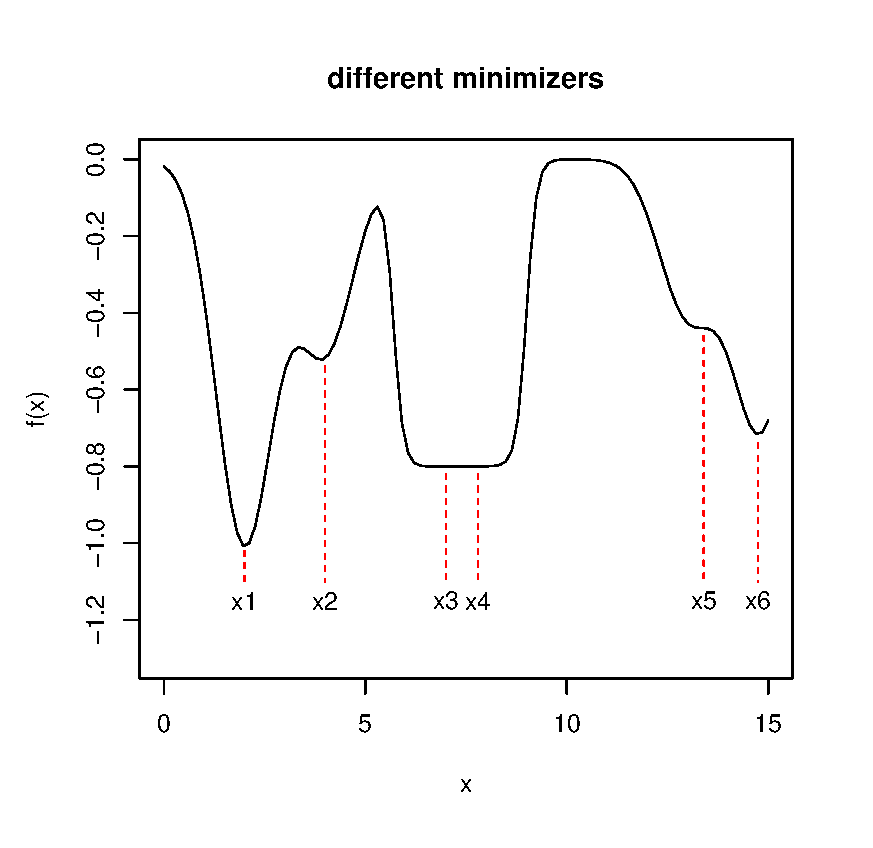
\includegraphics[width=3.0in]
		{02Background/opt/minimizers.png}
	\end{center}
	\caption[ค่าทำให้น้อยที่สุดต่าง ๆ]{ค่าทำให้น้อยที่สุดต่าง ๆ ของปัญหา $\mathrm{min}_x \; f(x)$. ค่าน้อยที่สุดของ $x$ หรือ $x_{\min} = -\infty$ แต่ค่าทำให้น้อยที่สุด $x^\ast = x_1$. ค่า $x_2, x_3, x_4, x_5, x_6$ เป็นค่าทำให้น้อยที่สุดท้องถิ่น. }
	\label{fig: opt minimizers}
\end{figure}
%



\subsection{การแก้ปัญหาด้วยวิธีลงเกรเดียนต์}
\label{sec: opt grad desc}
\index{thai}{วิธีลงเกรเดียนต์}
\index{english}{gradient descent algorithm}
\index{english}{optimization!gradient descent algorithm}
\index{thai}{การหาค่าดีที่สุด!วิธีลงเกรเดียนต์}

ศาสตร์\textit{การหาค่าดีที่สุด}นั้นกว้างขวาง
และมีการประยุกต์ใช้ที่หลากหลาย.
สำหรับการประยุกต์ใช้กับงาน\textit{การรู้จำรูปแบบ}
และ\textit{การเรียนรู้ของเครื่อง}
ลักษณะปัญหา มักจะถูกตีกรอบออกมาให้ตัวแปรตัดสินใจ $\bm{v} \in \mathbb{R}^n$ เมื่อ $n$ เป็นจำนวนเต็มมีค่าตั้งแต่หนึ่งขึ้นไป
และฟังก์ชันจุดประสงค์ 
%$g: \mathbb{R}^n \mapsto \mathbb{R}$ 
%โดยฟังก์ชัน 
$g$ เป็น\textit{ฟังก์ชันที่สามารถหาอนุพันธ์ได้} (differentiable function).
การมีฟังก์ชันจุดประสงค์ที่สามารถหาอนุพันธ์ได้
ช่วยให้สามารถใช้ขั้นตอนวิธีแก้ปัญหาค่าน้อยที่สุด
ที่มีประสิทธิภาพได้.

\textbf{วิธีลงเกรเดียนต์} (gradient descent algorithm) เป็น\textit{ขั้นตอนวิธี} (algorithm) สำหรับปัญหาค่าน้อยที่สุด.
\textit{วิธีลงเกรเดียนต์}เป็นขั้นตอนวิธีที่เรียบง่าย และใช้ได้ผลดี โดยเฉพาะกับปัญหาขนาดไม่ใหญ่มาก.
แนวคิดของ\textit{วิธีลงเกรเดียนต์} 
คือ
การใช้ค่าเกรเดียนต์
ช่วยในการหาค่าของ\textit{ตัวแปรตัดสินใจ}
โดย การเริ่มต้นด้วย
\textit{ค่าของตัวแปรตัดสินใจ} ค่าหนึ่ง
และคำนวณค่าเกรเดียนต์ ณ จุดนั้นออกมา
แล้วใช้ค่าเกรเดียนต์ที่ได้ บอกทิศทางในการปรับค่าของ\textit{ตัวแปรตัดสินใจ} ว่าควรปรับเพิ่มหรือลด มากน้อยเท่าไร 
ดำเนินการปรับค่าตัวแปรตัดสินใจ
และวนทำไปเรื่อย ๆ 
จนพบจุดที่เป็น\textit{ค่าทำให้น้อยที่สุด}.

เกรเดียนต์ 
ซึ่งเป็นอนุพันธ์ของฟังก์ชันจุดประสงค์ต่อตัวแปรตัดสินใจ
จะบอกอัตราการเปลี่ยนค่าของฟังก์ชันจุดประสงค์
เมื่อตัวแปรตัดสินใจเพิ่มค่าขึ้น.
ดังนั้นหาก{เกรเดียนต์}เป็นบวกและมีค่ามาก
นั่นหมายถึง 
ถ้าเพิ่มค่าตัวแปรตัดสินใจขึ้น
แล้วฟังก์ชันจุดประสงค์จะมีค่าเพิ่มขึ้นมาก.
หากค่าของ{เกรเดียนต์}เป็นบวกแต่มีขนาดเล็ก
การเพิ่มค่าตัวแปรตัดสินใจขึ้น
จะไปเพิ่มค่าฟังก์ชันจุดประสงค์ขึ้น แต่ไม่มาก
และหากเกรเดียนต์เป็นลบ
เมื่อเพิ่มค่าตัวแปรตัดสินใจขึ้น
ค่าฟังก์ชันจุดประสงค์จะลดลง.
ดังนั้นเกรเดียนต์จึงสามารถใช้เป็นเสมือนเงื่อนงำ 
ที่บอกทิศทางที่จะปรับค่า\textit{ตัวแปรตัดสินใจ} เพื่อลดค่าฟังก์ชันจุดประสงค์ลงไปเรื่อย ๆ
จนไปถึงค่าฟังก์ชันจุดประสงค์ที่น้อยที่สุดได้.
สมการ~\ref{eq: opt gd} 
แสดงการคำนวณค่าตัวแปรตัดสินใจ
ด้วยวิธีลงเกรเดียนต์
\begin{eqnarray}
\bm{v}^{(k+1)}
&=&
\bm{v}^{(k)} - \alpha \nabla g(\bm{v}^{(k)})
\label{eq: opt gd}
\end{eqnarray}
เมื่อ 
ตัวแปร $\bm{v}^{(k+1)}$
เป็นค่าใหม่ของตัวแปรตัดสินใจ (ที่ได้จากการคำนวณครั้งที่ $k+1$)
และ
ตัวแปร $\bm{v}^{(k)}$
เป็นค่าเดิมของตัวแปรตัดสินใจ (ที่ได้จากการคำนวณครั้งที่ $k$)
และ
เกรเดียนต์
$\nabla g(\bm{v}^{(k)})$
คือค่าเกรเดียนต์ของฟังก์ชันจุดประสงค์
ที่ค่าเดิมของตัวแปรตัดสินใจ 
(ค่าตัวแปรตัดสินใจที่ได้จากการคำนวณครั้งที่ $k$)
และค่าสเกล่าร์ $\alpha > 0$ เรียกว่า \textbf{ขนาดก้าว} (step size)
\index{thai}{ขนาดก้าว}
\index{english}{step size}
เป็นค่าที่ใช้ควบคุมอัตราเร็วในการปรับค่าของตัวแปรตัดสินใจ.

แนวคิดนี้ อุปมาเหมือน คนที่อยู่บนยอดเขาสูง 
ที่หมอกลงมากจนมองอะไรไม่เห็น 
และต้องการกลับบ้านที่อยู่พื้นล่าง.
เปรียบฟังก์ชันจุดประสงค์
เป็นเหมือนระดับความสูงของพื้นที่ ณ จุดที่ยืนอยู่
และตัวแปรตัดสินใจเป็นเหมือนตำแหน่งเส้นรุ้งเส้นแวง (latitude-longitude location) ณ จุดที่ยืนอยู่
ตัวแปร $\bm{v}^{(k)}$ ก็เสมือนตำแหน่งที่ยืนอยู่ปัจจุบัน
และเกรเดียนต์ $\nabla g(\bm{v}^{(k)})$ ก็เหมือนความชัน
ณ ตำแหน่งที่ยืนปัจจุบัน
ที่บอกว่าทิศทางไหนที่รู้สึกว่าพื้นชันขึ้น.
ถ้าต้องการกลับบ้าน หรือไปตำแหน่งที่ระดับความสูงที่ต่ำที่สุด
วิธีคือ ขยับจากจุดที่ยืนปัจจุบันไปจุดใหม่
โดยขยับไปในทิศทางลง (ซึ่งคือ ทิศทางตรงข้ามกับทิศที่พื้นชันขึ้น ได้แก่ ทิศ $-\nabla g(\bm{v}^{(k)})$)
โดยต้องค่อย ๆ เดิน ค่อย ๆ ก้าวเล็ก ๆ เพราะถ้าก้าวยาวเกินไป อาจก้าวข้ามทางเดินลงเขาแคบ ๆ ที่จะกลับบ้านได้ และ\textit{ขนาดก้าว} $\alpha$ ก็เป็นค่าที่ใช้คุมไม่ให้ก้าวยาวเกินไป
หลังจากก้าวไปแล้ว
ตอนนี้ ตำแหน่งที่ยืนก็จะเปลี่ยนใหม่เป็น $\bm{v}^{(k+1)}$
และก็ขยับแบบนี้อีก ทำซ้ำเรื่อย ๆ จนกลับถึงบ้าน.

\paragraph{ตัวอย่าง.}
การหา\textit{ค่าทำให้น้อยที่สุด}ของ $f(x) = - e^{ - (x-5)^2 }$ ด้วยวิธีลงเกรเดียนต์.
%
	\begin{itemize}
		\item
	เริ่มต้นด้วยการเลือกจุดเริ่มต้น สมมติเลือก $x^{(0)} = 6.5$ และเลือกใช้ค่าขนาดก้าว
	สมมติเลือกเป็น $\alpha = 0.5$.
	เกรเดียนต์สามารถวิเคราะห์การคำนวณไว้ได้
		\begin{eqnarray}
		\nabla f(x) &=& 
		\frac{d f(x)}{d x} = - e^{ - (x-5)^2 } \cdot (-2 x + 10).
		\nonumber   
		\end{eqnarray} 
%	
		\item ปรับค่าตัวแปรตัดสินใจ ตามสมการ~\ref{eq: opt gd}
		\\ 
		\begin{eqnarray}
		%(k=1) 
		&\;& \mbox{การคำนวณครั้งแรก } (k=1)
		\nonumber \\
		x^{(1)} &=& x^{(0)} - (0.5) \cdot \nabla f (x^{(0)})
%		\nonumber \\
%		&=& 
		= 6.5 - (0.5) \cdot \nabla f (6.5) 
		\nonumber \\ 
		&=& 6.5 - (0.5) \cdot \left(- e^{ - (6.5-5)^2 } \cdot (-2 \cdot (6.5) + 10) \right) 
		= 6.3419.
		\nonumber
\\		
%		\end{eqnarray}
%		\begin{eqnarray}
		%(k=2) 
		&\;& \mbox{การคำนวณที่สอง } (k=2)
\nonumber \\
		x^{(2)} &=& x^{(1)} - (0.5) \cdot \nabla f (x^{(1)})
%\nonumber \\
%&=& 
 = 6.3419 - (0.5) \cdot \nabla f (6.3419) = 6.1202
\nonumber
\\
%		\end{eqnarray}
%		\begin{eqnarray}	
%		&\;& \mbox{การคำนวณที่สาม } (k=3)
		&\;& \mbox{การคำนวณต่อ ๆ มา}
\nonumber \\
		x^{(3)} &=& 6.1202 - (0.5) \cdot \nabla f (6.1202) = 5.8009
\nonumber
%		\end{eqnarray}
%		\begin{eqnarray}	
%		&\;& \mbox{การคำนวณที่สี่ } (k=4)
%		&\;& \mbox{การคำนวณต่อ ๆ มา}
%\nonumber 
\\
x^{(4)} &=& 5.8009 - (0.5) \cdot \nabla f (5.8009) = 5.3792
\nonumber 
%\\
\end{eqnarray}
%
และ $x^{(5)} = 5.0508$;
$x^{(6)} = 5.0001$;
$x^{(7)} = 5.0000$;
$x^{(8)} = 5.0000$.
%\begin{eqnarray}	
%		&\;& \mbox{การคำนวณที่ห้า } (k=5)
%\nonumber \\
%		x^{(5)} &=& 5.0508   
%\end{eqnarray}
%\begin{eqnarray}	
%\nonumber \\
%		&\;& \mbox{การคำนวณที่หก } (k=6)
%\nonumber \\   
%x^{(6)} &=& 5.0001   
%\nonumber \\   
%		&\;& \mbox{การคำนวณที่เจ็ด } (k=7)
%\nonumber \\
%x^{(7)} &=& 5.0000   
%\nonumber \\   
%		&\;& \mbox{การคำนวณที่แปด } (k=8)
%\nonumber \\
%x^{(8)} &=& 5.0000   
%\nonumber
%		\end{eqnarray}
%		
		\item และผลลู่เข้าสู่ $x = 5$ ซึ่งคือ\textit{ค่าทำให้น้อยที่สุด}.
		ส่วน $f(5) = -1$ เป็นค่าฟังก์ชันจุดประสงค์ที่น้อยที่สุด 
		และค่าเกรเดียนต์ ณ จุดนี้คือ $\nabla f(5) = 0$.
	\hfill $\square$
	\end{itemize}
%	
สังเกตว่า ที่ค่าทำให้น้อยที่สุด $x^\ast$ จะทำให้เกรเดียนต์ $\nabla f(x^\ast) = 0$
และนี่คือ ธรรมชาติ%
\footnote{%
	นี่คือ \textit{เงื่อนไขจำเป็นอันดับแรก} (First-Order Necessary Condition).
	ดู \cite{ChongZak2ndEd} สำหรับรายละเอียด.
}
ของ\textit{ค่าทำให้น้อยที่สุด}
ซึ่งคือ
ณ จุด\textit{ค่าทำให้น้อยที่สุด}
เกรเดียนต์จะมีค่าเป็นศูนย์%
\footnote{%
เกรเดียนต์ $\nabla f(x^\ast) = 0$
เป็นจริง 
ในกรณีทั่วไปของปัญหาค่าน้อยที่สุดแบบไม่มีข้อจำกัด.
หัวข้อ~\ref{sec: opt contrained opt} อภิปรายกรณีปัญหาค่าน้อยที่สุดแบบมีข้อจำกัด
และแบบฝึกหัด~\ref{ex: opt min problem piecewise} แสดงตัวอย่างกรณีพิเศษ
ที่  
ณ จุด\textit{ค่าทำให้น้อยที่สุด}
แต่ค่าเกรเดียนต์ไม่เป็นศูนย์.
}
ดังนั้น ถึงแม้จะคำนวณต่อ
ค่าของตัวแปรตัดสินใจก็จะยังคงติดอยู่ที่\textit{ค่าทำให้น้อยที่สุด}.

\paragraph{การใช้งานวิธีลงเกรเดียนต์.}
\textit{วิธีลงเกรเดียนต์} มี\textit{อภิมานพารามิเตอร์}
เป็นค่า\textit{ขนาดก้าว}.
\index{thai}{อภิมานพารามิเตอร์}
\index{thai}{พารามิเตอร์!อภิมาน}
\index{english}{meta-parameter}
\index{english}{hyper-parameter}
\index{english}{parameter!meta-}
\index{english}{parameter!hyper-}
%
\textbf{อภิมานพารามิเตอร์}
(meta-parameter หรือ hyper-parameter)
หมายถึง ปัจจัยระดับสูงของวิธีการคำนวณ แต่ละวิธี
ที่ผู้ใช้ต้องเลือกให้เหมาะสม.
สำหรับ\textit{วิธีลงเกรเดียนต์}
ผู้ใช้ต้องเลือกค่าของ\textit{ขนาดก้าว}.
ถ้าเลือกใช้\textit{ขนาดก้าว}ที่มีค่าเล็กพอ
\textit{วิธีลงเกรเดียนต์}
จะรับประกัน\textit{การลู่เข้าได้}%
\footnote{%
\textit{วิธีลงเกรเดียนต์}
รับประกันการลู่เข้าสู่ค่าทำน้อยที่สุดท้องถิ่น
เมื่อเลือกใช้ขนาดก้าวที่มีค่าเล็กพอ
แต่ไม่ได้รับประกันว่า
จะเจอค่าทำน้อยที่สุดทั่วหมด
หรือไม่ได้รับประกันว่า จะไม่ไปติดอยู่\textit{จุดอานม้า} เป็นต้น.
}.
\textbf{การลู่เข้า} (convergence)
\index{english}{convergence}
\index{thai}{การลู่เข้า}
หมายถึง พฤติกรรมที่ดีของผลการคำนวณ
สำหรับ\textit{การคำนวณลักษณะการวนซ้ำขัดเกลา} (iterative refinement computation)
นั่นคือ
ค่าของผลการคำนวณของแต่ละรอบคำนวณ
มีการเปลี่ยนแปลงน้อยลง เมื่อรอบการคำนวณเพิ่มมากขึ้น
อาจกล่าวได้ว่า
การลู่เข้าคือพฤติกรรมที่ ผลลัพธ์จากการคำนวณเปลี่ยนแปลงค่าเข้าหา(ลู่เข้าหา)ค่าใดค่าหนึ่ง ในลักษณะคงที่
เมื่อรอบการคำนวณเพิ่มมากขึ้น.

\textit{ขนาดก้าว}ที่ใหญ่เกินไป อาจทำให้การคำนวณล้มเหลวได้
แต่\textit{ขนาดก้าว}ที่เล็กเกินไป อาจทำให้ต้องทำการคำนวณหลายรอบมาก ๆ 
ซึ่งมีผลให้ใช้เวลาในการคำนวณนาน
(ดูแบบฝึกหัด~\ref{ex: opt gd step size} ประกอบ).
ในทางปฏิบัติ
เพื่อให้ไม่เสียเวลาคำนวณมากเกินไป
\textbf{เงื่อนไขการจบ}การคำนวณ (terminating condition)
มักถูกใช้ประกอบ.
\index{english}{terminating condition}
\index{thai}{เงื่อนไขการจบ}
%
\textit{เงื่อนไขการจบ}ที่นิยมใช้กับ\textit{วิธีลงเกรเดียนต์}
ได้แก่ เงื่อนไข\textit{จำนวนรอบสูงสุด} (maximum number of iterations)
และ
เงื่อนไข\textit{ความคลาดเคลื่อนยินยอม} (tolerance).

เงื่อนไข\textit{จำนวนรอบสูงสุด}
จะกำหนดจำนวนรอบที่จะหยุดทำการคำนวณ
ไม่ว่าการคำนวณนั้น จะดำเนินไปถึงสิ้นสุดหรือไม่ จะได้\textit{ค่าทำให้น้อยที่สุด}แล้วหรือไม่.
นั่นคือ กำหนด
$\bm{v}^{(k+1)} = \bm{v}^{(k)} - \alpha \nabla g (\bm{v}^{(k)})$ สำหรับ $k = 1, \ldots, N_{\max}$
เมื่อ $N_{\max}$ คือจำนวนรอบคำนวณที่มากที่สุด
และการใช้เงื่อนไขนี้ จะทำให้ผู้ใช้ต้องกำหนด\textit{จำนวนรอบสูงสุด}นี้ด้วย.
ดังนั้น\textit{อภิมานพารามิเตอร์}
จะมี\textit{จำนวนรอบสูงสุด}ขึ้นอีกตัว.

\textit{เงื่อนไขความคลาดเคลื่อนยินยอม}
กำหนดค่าความคลาดเคลื่อนที่ยอมรับได้ ซึ่งอาจเลือกใช้เงื่อนไข 
ขนาดของเกรเดียนต์
$\epsilon = \|\nabla g(\bm{v}^{(k+1)})\|$.
แบบฝึกหัด~\ref{ex: opt gd simple code}
แสดงตัวอย่างโปรแกรม\textit{วิธีลงเกรเดียนต์}อย่างง่าย
ที่ใช้\textit{เงื่อนไขการจบ}แค่\textit{จำนวนรอบสูงสุด}.
แบบฝึกหัด~\ref{ex: opt gd termination code} 
แสดงตัวอย่างโปรแกรม\textit{วิธีลงเกรเดียนต์}ที่ใช้\textit{เงื่อนไขคลาดเคลื่อนยินยอม}.

\textit{วิธีลงเกรเดียนต์}ประยุกต์ใช้ได้ง่าย
ต้องการแค่เกรเดียนต์ และค่าเริ่มต้น.
ค่าเริ่มต้นก่อนการคำนวณของตัวแปรตัดสินใจ 
อาจเป็นค่าใดก็ได้%
\footnote{%
\textit{วิธีลงเกรเดียนต์}ทนทานต่อค่าเริ่มต้นต่าง ๆ
ในแง่ที่ว่า โดยทั่วไปแล้ว (ถ้าปัญหาไม่ยากเกินไป)
\textit{วิธีลงเกรเดียนต์}จะสามารถหา\textit{ค่าทำให้น้อยที่สุด}ได้
แม้เลือกค่าเริ่มต้นต่างกัน
แต่การเลือกค่าเริ่มต้นที่ดี
จะช่วยให้\textit{วิธีลงเกรเดียนต์}ทำงานได้เร็วขึ้น
และสำหรับหลาย ๆ กรณี
ค่าเริ่มต้นต่างกันอาจนำไปสู่\textit{ค่าทำให้น้อยที่สุดท้องถิ่น}คนละตัว (กรณีปัญหา\textit{หลายภาวะ} multi-modal problem ดูแบบฝึกหัด~\ref{ex: opt gd init} เพิ่มเติม)
หรือสำหรับบางกรณี
ค่าเริ่มต้นบางค่า อาจทำให้\textit{วิธีลงเกรเดียนต์}ไม่สามารถทำงานได้เลย.
ดูแบบฝึกหัด~\ref{ex: opt gd init} ประกอบ.
}
แต่โดยทั่วไป มักนิยมใช้\textbf{การกำหนดค่าเริ่มต้น} (initialization) ให้กับ\textit{ตัวแปรตัดสินใจ}
ด้วยค่าที่สุ่มขึ้นมา.
(ดูแบบฝึกหัด~\ref{ex: opt gd random.norm init})

ปัญหาที่ตัวแปรตัดสินใจมีหลาย ๆ ตัว 
สามารถใช้วิธีลงเกรเดียนต์ได้
โดยการจัดหลาย ๆ ตัวแปรตัดสินใจ 
เข้ามารวมกันเป็นเวกเตอร์ตัวแปรตัดสินใจเวกเตอร์เดียว
และวิธีลงเกรเดียนต์เตรียมการมาสำหรับกรณีนี้อยู่แล้ว 
(สมการ~\ref{eq: opt gd}).
สังเกตว่า ตัวแปรตัดสินใจเขียนเป็นเวกเตอร์
และอัตราการเปลี่ยนก็ใช้เกรเดียนต์
แต่การนำ\textit{วิธีลงเกรเดียนต์}
ไปเขียนโปรแกรมเพื่อทำงานกับเวกเตอร์
จะต้องระวังเรื่องของตัวแปรเป็นพิเศษ. 
(ดูแบบฝึกหัด~\ref{ex: opt gd vec code} ประกอบ)
นอกจากนั้น เพื่อช่วยให้สามารถตรวจสอบความก้าวหน้า
ในการหา\textit{ค่าทำให้น้อยที่สุด}ได้อย่างมีประสิทธิภาพ ควรตรวจสอบ\textit{ค่าฟังก์ชันจุดประสงค์}ทุก ๆ รอบคำนวณ.
ตัวอย่างต่อไปนี้ แสดงการคำนวณของ\textit{วิธีลงเกรเดียนต์} เมื่อตัวแปรตัดสินใจมีสองค่า.

%
\begin{figure}
	\begin{center}
		\begin{tabular}{cc}
			\includegraphics[width=3.0in]
			{02Background/opt/code_opt_2Dcontour.png}
			&
			\includegraphics[width=3.0in]
			{02Background/opt/code_opt_2Dpersp.png}\\\
			ก & ข	
		\end{tabular}
	\end{center}
	\caption[ภาพคอนทัวร์และภาพสามทัศนมิติของฟังก์ชันจุดประสงค์]{ภาพคอนทัวร์ (ก) และภาพสามทัศนมิติ (ข) ของฟังก์ชันจุดประสงค์ $g(\bm{v}) = -e^{-53-v_1^2 -2v_2^2-v_1 v_2 + 10 v_1 + 19 v_2}$}
	\label{fig: opt 2D}
\end{figure}

\paragraph{ตัวอย่าง เมื่อตัวแปรตัดสินใจเป็นเวกเตอร์.}
%จงใช้วิธีลงเกรเดียนต์ 
%เพื่อแก้
ปัญหา เช่น $\min_{\bm{v}} \; g$ เมื่อ
$\bm{v} =[v_1, v_2]^T$
และ
$g(\bm{v}) = -e^{-53-v_1^2 -2v_2^2-v_1 v_2 + 10 v_1 + 19 v_2}$
ซึ่งรูป~\ref{fig: opt 2D} แสดงฟังก์ชันจุดประสงค์ในรูปคอนทัวร์ (contour plot) และในรูปสามทัศนมิติ (3d perspective plot)
ปัญหานี้สามารถแก้ด้วยวิธีลงเกรเดียนต์ ดังนี้.

	\begin{itemize}
	\item
	เลือก\textit{อภิมานพารามิเตอร์}
	ได้แก่ ค่าขนาดก้าว $\alpha = 0.01$

	\item 
	เตรียมฟังก์ชันคำนวณเกรเดียนต์
	\begin{eqnarray}
	\nabla g(\bm{v}) &=& 
	\begin{bmatrix}
	\frac{\partial g}{\partial v_1} \\
	\frac{\partial g}{\partial v_2}
	\end{bmatrix}
	= 
	\begin{bmatrix}
g(\bm{v}) \cdot (-2 v_1 - v_2 + 10) \\
g(\bm{v}) \cdot (-4 v_2 - v_1 + 19)
\end{bmatrix}
= g(\bm{v}) \cdot 
\begin{bmatrix}
-2 v_1 - v_2 + 10
\\
-4 v_2 - v_1 + 19
\end{bmatrix}
	\nonumber .  
	\end{eqnarray} 
สังเกต ค่าฟังก์ชันจุดประสงค์ $g(\bm{v})$ เป็นสเกล่าร์
แต่ค่าเกรเดียนต์ $\nabla g(\bm{v})$ เป็นเวกเตอร์ ที่มีสัดส่วน (จำนวนส่วนประกอบ) เท่ากับสัดส่วนของตัวแปรตัดสินใจ $\bm{v}$.
	
\item สุ่มเลือกค่าเริ่มต้น สมมติว่าสุ่มได้ $\bm{v}^{(0)} = [2.5, 3.5]^T$

\item ปรับค่าตัวแปรตัดสินใจ ตามสมการ~\ref{eq: opt gd}
	\\ 
	\begin{eqnarray}
	%(k=1) 
	&\;& \mbox{การคำนวณครั้งแรก } (k=1)
	\nonumber \\
	\bm{v}^{(1)} &=& \bm{v}^{(0)} - (0.01) \cdot \nabla g (\bm{v}^{(0)})
	\nonumber \\
	&=& [2.5, 3.5]^T - 0.01 \cdot (-0.3679) \cdot [-2(2.5)-3.5+10, -4(3.5)-2.5+19]^T
	\nonumber \\
	&=& [2.5, 3.5]^T - 0.01 \cdot [-0.5518,
	-0.9197]^T = [2.506, 3.509]^T
\nonumber \\	
	&\;& \mbox{การคำนวณที่สอง } (k=2)
\nonumber \\		
	\bm{v}^{(2)} &=& \bm{v}^{(1)} - (0.01) \cdot \nabla g (\bm{v}^{(1)})
\nonumber \\	
&=& [2.506, 3.509]^T - 0.01 \cdot [-0.5615, -0.9326]^T = [2.511, 3.519]^T
\nonumber \\
	&\;& \mbox{การคำนวณที่สาม } (k=3)
	\nonumber \\
	\bm{v}^{(3)} &=& \bm{v}^{(2)} - (0.01) \cdot \nabla g (\bm{v}^{(2)})
\nonumber \\	
&=& [2.511, 3.519]^T - 0.01 \cdot [-0.5711, -0.9452]^T = [2.517, 3.528]^T
\nonumber 
	\nonumber
	\end{eqnarray}
	
	\item และเมื่อดำเนินการคำนวณต่อไป
	(ดูแบบฝึกหัด~\ref{ex: opt gd vec code} ประกอบ)
	จะพบว่า 
%	$\bm{v}^{(100)} = [2.928, 4.013]^T$,
%	$\bm{v}^{(200)} = [2.987, 4.005]^T$,
	$\bm{v}^{(300)} = [2.997, 4.001]^T$,
	$\bm{v}^{(400)} = [2.999, 4.000]^T$,
	$\bm{v}^{(500)} = [3.000, 4.000]^T$,
	$\bm{v}^{(600)} = [3.000, 4.000]^T$.
	ค่าของ $\bm{v}$ ปรับน้อยมาก ๆ จนถึงแทบไม่ปรับเลยในรอบคำนวณหลัง ๆ นี่คือ $\bm{v}$ ลู่เข้าหา $[3, 4]^T$.
	รูป~\ref{fig: opt gd 2D trajectory} แสดงการปรับค่าตัวแปรตัดสินใจ ในรูปเส้นทางบนภาพคอนทัวร์%
	\footnote{รูปเส้นทางบนภาพคอนทัวร์ เช่นนี้ สามารถแสดงได้เฉพาะกรณีที่ตัวแปรตัดสินใจ $\bm{v} \in \mathbb{R}^2$ หากตัวแปรตัดสินใจอยู่ในมิติปริภูมิที่ใหญ่ขึ้น การนำเสนอด้วยภาพจะทำได้ยากมาก.}
	ของฟังก์ชันจุดประสงค์.
	รูป~\ref{fig: opt gd 2D} แสดง \textit{ความก้าวหน้า} (progress) ของการดำเนินการหาค่าทำให้น้อยที่สุด.
	\hfill $\square$
\end{itemize}

จากรูป~\ref{fig: opt gd 2D} 
ค่าของ\textit{ตัวแปรตัดสินใจ} $\bm{v}$ ทั้งสองค่า 
จะปรับเข้าหา $[3, 4]^T$
นั่นคือคำตอบลู่เข้า.
เมื่อดูที่จุดลู่เข้า  ดังที่ได้อภิปรายมาแล้ว
ขนาดของเกรเดียนต์จะเป็นศูนย์ที่\textit{จุดดีที่สุด} (optimal point)
\index{thai}{จุดที่ดีที่สุด}
\index{english}{optimal point}
ซึ่งเป็นจุดที่\textit{ตัวแปรตัดสินใจ}ปรับค่าไปอยู่ที่\textit{ค่าทำให้น้อยที่สุด}.
ขนาดของเกรเดียนต์จึงนิยมใช้เป็นเงื่อนไขในการจบโปรแกรม เพื่อไม่ต้องคำนวณมากรอบเกินไป เช่นกรณีนี้ จะเห็นว่าทำการคำนวณแค่ราว ๆ $500$ รอบก็เห็นการลู่เข้าชัดเจนแล้ว.
เมื่อดูที่ฟังก์ชันจุดประสงค์ (ภาพ Loss บนซ้าย) ค่าฟังก์ชันจุดประสงค์จะน้อยลงเรื่อย ๆ ถ้าเลือกค่า\textit{ขนาดก้าว}ไม่ใหญ่เกินไป.
พฤติกรรมการทำงานของ\textit{วิธีลงเกรเดียนต์}จะมีลักษณะเช่นนี้ คือ 
ค่าฟังก์ชันจุดประสงค์จะลดลง เมื่อรอบคำนวณเพิ่มขึ้น.
การดูค่าฟังก์ชันจุดประสงค์ต่อรอบคำนวณเช่นนี้
สะดวก เพราะสามารถตรวจสอบได้ ไม่ว่าตัวแปรตัดสินใจจะมีจำนวนเท่าใด
และถูกใช้เป็นแนวทางปฎิบติ
เพื่อติดตามความก้าวหน้า
และวิเคราะห์การทำงานของการแก้ปัญหาค่าน้อยที่สุด ว่าดำเนินการได้ดีมากน้อยเพียงใด.

%
\begin{figure}
	\begin{center}
		\includegraphics[width=0.75\textwidth]
		{02Background/opt/code_opt_2Dgd_trajectory.png}
	\end{center}
	\caption[เส้นทางการหาค่าทำให้น้อยที่สุด]{เส้นทางการหา\textit{ค่าทำให้น้อยที่สุด} จุดวงกลมสีดำแสดงจุดเริ่มต้น (ตำแหน่ง $[2.5, 3.5]^T$) และจุดดาวสีแดงแสดงจุดสุดท้าย (ตำแหน่ง $[3, 4]^T$). เส้นทางระหว่างจุดทั้งสอง คือค่าต่าง ๆ ที่ตัวแปรตัดสินใจถูกปรับตั้งแต่รอบคำนวณแรก ๆ ไปจนถึงรอบคำนวณท้าย ๆ.
	}
	\label{fig: opt gd 2D trajectory}
\end{figure}
%


%
\begin{figure}
	\begin{center}
		\includegraphics[width=0.75\textwidth]
		{02Background/opt/code_opt_2Dgd_progress.png}
	\end{center}
	\caption[ความก้าวหน้าในการหาค่าทำให้น้อยที่สุด]{\textit{ความก้าวหน้า}ในการหา\textit{ค่าทำให้น้อยที่สุด}. 
	ภาพบนซ้าย (\texttt{Loss}) แสดงค่าฟังก์ชันจุดประสงค์ต่อรอบการคำนวณ. 
	ภาพล่างซ้าย (\texttt{|grad|}) แสดงขนาดเกรเดียนต์ต่อรอบการคำนวณ.
	ขนาดเกรเดียนต์นิยมใช้เป็น\textit{เงื่อนไขการจบ} เพื่อลดเวลาคำนวณลง.
	ภาพขวาแสดงค่า\textit{ตัวแปรตัดสินใจ}ต่อรอบการคำนวณ ภาพบนแสดง $v_1$ และภาพล่างแสดง $v_2$.
    }
	\label{fig: opt gd 2D}
\end{figure}
%


%วิธีลงเกรเดียนต์นั้น นอกจากใช้งานได้ดีกับปัญหาค่าน้อยที่สุดแล้ว
%ยังใช้ได้ดีกับชีวิตด้วย
\begin{quote}
วิธีลงเกรเดียนต์:\\
``ไม่ว่าเราเริ่มต้นอยู่ที่ไหน ถ้าเราขยับไปทิศทางที่ดีขึ้นเรื่อย ๆ
\\
เราจะไปถึงจุดที่ดีที่สุดได้
เพียงต้องทำเรื่อย ๆ และไม่รีบเกินไป''
\end{quote}
\index{english}{quote!gradient descent}



\subsection{การหาค่าดีที่สุดแบบมีข้อจำกัด}
\label{sec: opt contrained opt}
\index{english}{constrained optimization}
\index{thai}{การหาค่าดีที่สุดแบบมีข้อจำกัด}
\index{english}{optimization!constrained}
\index{thai}{การหาค่าดีที่สุด!แบบมีข้อจำกัด}

\textit{การหาค่าดีที่สุด}ที่ได้อภิปรายมา
ค่าของตัวแปรตัดสินใจเป็นค่าจำนวนจริงใด ๆ
ซึ่งเขียนเป็นสัญกรณ์ทั่ว ๆ ไป $\mathrm{min}_{\bm{v}} g(\bm{v})$ โดย $\bm{v} \in \mathbb{R}^n$ เมื่อ $n$ เป็นจำนวนเต็มที่มีค่าตั้งแต่หนึ่งเป็นต้นไป
\textit{การหาค่าดีที่สุด}แบบนี้ 
ไม่ได้มีเงื่อนไขจำกัดค่าของตัวแปรตัดสินใจ (นอกจากเป็นจำนวนจริง)
และ\textit{การหาค่าดีที่สุด}แบบนี้ จะเรียกว่า
\textbf{การหาค่าดีที่สุดแบบไม่มีข้อจำกัด} (unconstrained optimization).

กรณีที่มีข้อจำกัดของค่าของตัวแปรตัดสินใจ
จะเรียกว่า
\textbf{การหาค่าดีที่สุดแบบมีข้อจำกัด} (constrained optimization)
และจะใช้สัญกรณ์ เพื่อระบุข้อจำกัดอย่างชัดเจน เช่น
\begin{eqnarray}
\underset{\bm{v}}{\mathrm{minimize}} & g(\bm{v})
\nonumber \\
\mbox{subject to} & \bm{v} \in \Omega 
\label{eq: opt contrained opt}
\end{eqnarray}
เมื่อ $\bm{v} \in \mathbb{R}^n$ เป็นตัวแปรตัดสินใจ
ฟังก์ชัน $g: \mathbb{R}^n \rightarrow \mathbb{R}$ เป็นฟังก์ชันจุดประสงค์
และเซต $\Omega$ เป็นเซตย่อยของ $\mathbb{R}^n$ ที่ระบุค่าของตัวแปรตัดสินใจในช่วงที่สนใจ หรือกลุ่มค่าที่ยอมรับได้.
ค่าคำตอบของ $\bm{v}$ ที่ได้จะต้องอยู่ในเซตย่อยนี้.
เซต $\Omega$ นี้ เรียกว่า \textbf{เซตข้อจำกัด} (constraint set หรือ เซตที่เป็นไปได้ feasible set).
กรณีที่ $\Omega = \mathbb{R}^n$
ปัญหาในกรณีนี้จะเป็น
\textit{การหาค่าดีที่สุดแบบไม่มีข้อจำกัด}.
สัญกรณ์~\ref{eq: opt contrained opt} อาจเขียนย่อเป็น $\mathrm{min}_{\bm{v}} \; g(\bm{v}) \; \mbox{s.t.} \; \bm{v} \in \Omega$.

จากตัวอย่าง การหาอุณหภูมิบ่มทุเรียน ถ้ากำหนดว่า อุณหภูมิบ่มต้องอยู่ในช่วง $30$ ถึง $80$ องศาเซลเซียส (เพราะว่าเตาบ่มที่มี ทำอุณหภูมิได้ในช่วงแค่นั้น)
ปัญหานี้จะเป็น\textit{การหาค่าดีที่สุดแบบมีข้อจำกัด}
และอาจเขียนเป็น สัญกรณ์ $\mathrm{max}_t \; \mathrm{sugar}(t) \; \mbox{s.t.} \; 30 \leq t \leq 80$
เมื่อ $t$ แทนอุณหภูมิบ่มในหน่วยองศาเซลเซียส
ฟังก์ชัน $\mathrm{sugar}$ ประเมินระดับน้ำตาลที่ได้ จากการบ่มด้วยอุณหภูมิ $t$
และข้อจำกัด $30 \leq t \leq 80$ ระบุค่าของ $t$ ที่ใช้ได้ว่า อยู่ในช่วง $30$ ถึง $80$.
(ปัญหาค่ามากที่สุดนี้ เทียบเท่า
ปัญหาค่าน้อยที่สุด
$\mathrm{min}_t \; -\mathrm{sugar}(t) \; \mbox{s.t.} \; 30 \leq t \leq 80$
)

\paragraph{ค่าทำให้น้อยที่สุดท้องถิ่น และค่าทำให้มากที่สุดทั่วหมด.}
ในกรณีที่มีข้อจำกัด ค่าของตัวแปรตัดสินใจจะพิจารณาจากค่าที่\textit{เป็นไปได้} (feasible) เท่านั้น.
\textit{ค่าทำให้น้อยที่สุดท้องถิ่น}
คือ ค่าของตัวแปรตัดสินใจ ที่ทำให้ฟังก์ชันจุดประสงค์มีค่าน้อยกว่าหรือเท่ากับค่าฟังก์ชันจุดประสงค์ของค่าที่\textit{เป็นไปได้}บริเวณรอบ ๆ.
นั่นคือ
%\footnote{
%	สัญกรณ์ $\rho_1 \subset \rho_2$ บอกว่า เซต $\rho_1$ เป็นเซตย่อยของ $\rho_2$.
%	สัญกรณ์ $\rho_1 \setminus \rho_2$ เป็นการดำเนินการลบสมาชิก โดยผลลัพธ์คือ สมาชิกทุกตัวในเซต $\rho_1$ ที่ไม่ได้เป็นสมาชิกของเซต $\rho_2$.
%} 
ถ้ากำหนดให้ $g: \mathbb{R}^n \rightarrow \mathbb{R}$ เป็นฟังก์ชันค่าจริง 
ที่นิยามสำหรับเซต $\Omega \subset \mathbb{R}^n$
แล้ว จุด $\bm{v}^\ast \in \Omega$ เป็น\textit{ค่าทำให้น้อยที่สุดท้องถิ่น} ของฟังก์ชัน $g$ บนเซต $\Omega$ ถ้ามีค่า $\epsilon > 0$ ที่ $g(\bm{v}) \geq g(\bm{v}^\ast)$ สำหรับทุกค่าของ $\bm{v} \in \Omega \setminus \{ \bm{v}^\ast \}$
และ $\|\bm{v} - \bm{v}^\ast\| < \epsilon$.
ส่วน\textit{ค่าทำให้น้อยที่สุดทั่วหมด}
คือ ค่าของตัวแปรตัดสินใจ ที่ทำให้ฟังก์ชันจุดประสงค์มีค่าน้อยกว่าหรือเท่ากับค่าฟังก์ชันจุดประสงค์ของค่าที่\textit{เป็นไปได้}อื่น ๆ ทุกค่า.
นั่นคือ
จุด $\bm{v}^\ast \in \Omega$ จะเป็น\textit{ค่าทำให้น้อยที่สุดทั่วหมด}ของฟังก์ชัน $g$ บนเซต $\Omega$ ถ้า $g(\bm{v}) \geq g(\bm{v}^\ast)$ สำหรับ ทุกค่าของ $\bm{v} \in \Omega \setminus \{ \bm{v}^\ast \}$.

\paragraph{วิธีแก้ปัญหาค่าน้อยที่สุดแบบมีข้อจำกัด.}
มีสองแนวทางหลักที่ทั่วไปนิยมใช้แก้ปัญหาค่าน้อยที่สุดแบบมีข้อจำกัด คือ
\textit{แนวทางการแปลงมุมมอง}
และ\textit{แนวทางการลงโทษ}.
\index{english}{constrained optimization}
\index{english}{optimization!constrained}
\index{english}{constrained optimization!projection}
\index{english}{constrained optimization!penalty}
\index{thai}{การหาค่าดีที่สุดแบบมีข้อจำกัด!แนวทางการแปลงมุมมอง}
\index{thai}{การหาค่าดีที่สุดแบบมีข้อจำกัด!แนวทางการลงโทษ}

\textbf{แนวทางการแปลงมุมมอง} (projection approach)
จะใช้ฟังก์ชัน $F: \mathbb{R}^n \rightarrow \Omega$ เพื่อแปลงค่าของตัวแปรตัดสินใจมาเป็น\textit{ค่าที่เป็นไปได้}.
ตัวอย่าง เช่น เมื่อใชักับ\textit{วิธีลงเกรเดียนต์} อาจทำโดย
\begin{eqnarray}
\bm{v}^{(k+1)} = F \left( \bm{v}^{(k)} - \alpha \cdot \nabla g(\bm{v}^{(k)}) \right)
\label{eq: opt const projection} 
\end{eqnarray}
ในทางปฏิบัติแล้ว 
ฟังก์ชันแปลง $F$ นี้
อาจจะยากที่หา หรือยากที่จะคำนวณ
ในหลาย ๆ สถานการณ์.
งาน\textit{การเรียนรู้ของเครื่อง} มักนิยมใช้\textit{แนวทางการลงโทษ}มากกว่า.

\textbf{แนวทางการลงโทษ}
(penalty approach)
\index{english}{penalty method}
\index{thai}{วิธีการลงโทษ}
จะใช้การลงโทษ
เมื่อค่า\textit{ตัวแปรตัดสินใจ}ไม่อยู่ใน\textit{เซตข้อจำกัด}
โดยการปรับกรอบปัญหาจากเดิม $\min_{\bm{v}} g(\bm{v}) \; \mbox{s.t.} \; \bm{v} \in \Omega$
ไปเป็นกรอบปัญหาใหม่
\begin{eqnarray}
\underset{\bm{v}}{\mathrm{min}} \; g(\bm{v}) + \lambda P(\bm{v})
\label{eq: opt const penalty}
\end{eqnarray}
เมื่อ $\lambda \in \mathbb{R}$ 
เป็น\textbf{พารามิเตอร์ลงโทษ} (penalty parameter) ซึ่งนิยมเรียกว่า \textit{ลากรานจ์พารามิเตอร์} (Lagrange parameter)
\index{english}{Lagrange parameter}
\index{thai}{ลากรานจ์พารามิเตอร์}
และฟังก์ชัน $P: \mathbb{R}^n \rightarrow [0, \infty)$ เป็น\textit{ฟังก์ชันต่อเนื่อง} (continuous function)
เรียกว่า
\textbf{ฟังก์ชันลงโทษ} (penalty function)
\index{thai}{ฟังก์ชันลงโทษ}
\index{english}{penalty function}
โดย 
\textit{ฟังก์ชันลงโทษ}จะมีค่าเป็นศูนย์
เมื่อค่าตัวแปรตัดสินในอยู่ในเซตข้อจำกัด
นั่นคือ $P(\bm{v}') = 0$ สำหรับ $\bm{v}' \in \Omega$.

%ตัวอย่าง เช่นปัญหาบ่มทุเรียน
%$\min_t - \mathrm{sugar}(t) \; \mbox{s.t.} \; t \leq 80$
%ก็อาจจะถูกตีกรอบใหม่ตามแนวทางการลงโทษได้เป็น
%$\min_t - \mathrm{sugar}(t) + \lambda P_o (t)$
%เมื่อ

% np.sin(x)/(1 + x**2)
ตัวอย่างเช่น ปัญหา $\min_x \sin (x) /(1 + x^2) \; \mbox{s.t.} \; x \geq 0$.
รูป~\ref{fig: opt constrained problem} แสดงฟังก์ชันจุดประสงค์ 
%$\sin (x) /(1 + x^2)$
และแสดงส่วนที่ไม่ผ่านเงื่อนไขด้วยแรเงาสีเทา.
รูปแสดงให้เห็นว่า จุดที่ทำให้ค่าฟังก์ชันจุดประสงค์น้อยที่สุด มีค่าเป็นลบ แต่จุดนี้ละเมิดข้อจำกัด และใช้เป็นคำตอบไม่ได้.
การหาคำตอบด้วยวิธีลงโทษ
อาจเลือกใช้ฟังก์ชัน
\begin{eqnarray}
P(x) = \left \{ 
     \begin{array}{l l}
0 & \quad \mbox{เมื่อ} \quad x \geq 0, \\
-x & \quad \mbox{เมื่อ} \quad x < 0.
\end{array} 
\right.
\label{eq: opt const penalty function}
\end{eqnarray}
ซึ่งเป็นฟังก์ชันต่อเนื่อง (ทำให้สามารถหาอนุพันธ์ได้ และสามารถใช้วิธีแก้ปัญหา เช่น วิธีลงเกรเดียนต์ได้)
และฟังก์ชัน $P$ ลงโทษค่าที่ละเมิดข้อจำกัดตามปริมาณที่ละเมิด.
รูป~\ref{fig: opt penalty function} แสดงค่าของฟังก์ชันลงโทษในสมการ~\ref{eq: opt const penalty function}
และเมื่อนำฟังก์ชันลงโทษนี้
ไปใช้ร่วมกับฟังก์ชันจุดประสงค์
ฟังก์ชันที่ปรับใหม่จะเปลี่ยนพฤติกรรมไป
ดังแสดงในรูป~\ref{fig: opt penalized loss}.

วิธีใช้การลงโทษนี้ ก็คือ
การเปลี่ยนจาก\textit{ปัญหาแบบมีข้อจำกัด}
กลับมาเป็น\textit{ปัญหาแบบไม่มีข้อจำกัด}
โดย
การดัดแปลงฟังก์ชันจุดประสงค์ใหม่
เพื่อให้คำตอบ 
อยู่ในช่วงค่าที่\textit{เป็นไปได้}.
ดังนั้น ขั้นตอนการหาคำตอบต่อไป ก็สามารถดำเนินการได้
โดยใช้วิธีแก้ปัญหา แบบเดียวกับ\textit{ปัญหาแบบไม่มีข้อจำกัด}. % เช่น วิธีลงเกรเดียนต์ เป็นต้น.

รูป~\ref{fig: opt penalized loss} แสดงให้เห็นว่า
เมื่อ
ค่าของ\textit{ลากรานจ์พารามิเตอร์}ใหญ่มากพอ
\textit{ค่าทำน้อยที่สุด}ของฟังก์ชันจุดประสงค์ใหม่
จะถูกบังคับให้อยู่ในช่วงค่าที่\textit{เป็นไปได้}.
กลไกการทำงานของการลงโทษ คือ
การลงโทษจะทำให้
คำตอบของ\textit{ปัญหาค่าน้อยที่สุด}ใหม่ ที่รวม\textit{การลงโทษ}เข้าไป จะเป็น%
\footnote{%
กำหนดให้ $\bm{v}^{(k)}$ เป็นคำตอบของปัญหาที่มีการลงโทษด้วยค่า $\lambda_k$ 
และฟังก์ชันจุดประสงค์เดิม $g$ เป็นฟังก์ชันต่อเนื่อง
และ $\lambda_k \rightarrow \infty$
เมื่อ $k \rightarrow \infty$
แล้ว
\textit{ลิมิต} (limit) ของลำดับที่ลู่เข้า $\{ \bm{v}^{(k)} \}$ จะเป็นคำตอบของ\textit{ปัญหาแบบมีข้อจำกัด}เดิม. 
ดู \cite{ChongZak2ndEd} สำหรับรายละเอียด.
}%
คำตอบของ\textit{ปัญหาค่าน้อยที่สุดแบบมีข้อจำกัด}เดิม
เมื่อ\textit{ลากรานจ์พารามิเตอร์}มีค่าใหญ่มากพอ.

ในทางปฏิบัติ
การแก้ปัญหาด้วยวิธีลงโทษ จะเลือกค่าของ\textit{ลากรานจ์พารามิเตอร์}มาค่าหนึ่ง และดำเนินการแก้ปัญหา
แล้วตรวจสอบค่าคำตอบที่ได้ ว่าอยู่ภายใต้ข้อจำกัดหรือไม่
ถ้าคำตอบที่ได้ อยู่ภายใต้ข้อจำกัด นี่ก็คือ
คำตอบของปัญหาที่ใช้ได้.
แต่ถ้าคำตอบที่ได้ ไม่อยู่ภายใต้ข้อจำกัด
จะต้องเพิ่มค่าของ\textit{ลากรานจ์พารามิเตอร์}ขึ้น และดำเนินการแก้ปัญหาอีก และทำเช่นนี้ เพิ่มค่า\textit{ลากรานจ์พารามิเตอร์}ขึ้น
จนกว่าจะได้คำตอบที่อยู่ภายใต้ข้อจำกัด.


%นั่นคือ
%ถ้ากำหนดให้ 
%$\min_{\bm{v}} g(\bm{v}) 
%\mbox{ s.t. } \bm(v) \in \Omega$
%เป็นปัญหาแบบมีข้อจำกัด
%และ\textit{ปัญหาที่ถูกลงโทษ} (penalized problem) 
%ตีกรอบปัญหาเป็น 
%$\min_{\bm{v}} g(\bm{v}) + \lambda P(\bm(v))$
%เมื่อ $P(\bm{v})$ คือฟังก์ชันที่ลงโทษ $\bm{v} \notin \Omega$ 
%และ $\lambda$ คือลากรานจ์พารามิเตอร์
%และกำหนดให้ 
%$\bm{v}^{(k)}$ เป็นคำตอบของ\textit{ปัญหาที่ถูกลงโทษ} ใช้ค่าลากรานจ์ $\lambda_k$
%และ $g$ เป็น\textit{ฟังก์ชันต่อเนื่อง}
%และ $\

%เนื่องจาก\textit{วิธีการลงโทษ}ใช้การปรับตีกรอบ\textit{ฟังก์ชันจุดประสงค์}ใหม่
%เพื่อลดความสับสนและเพื่อความกระชับ
%จากนี้ไป อาจใช้คำว่า \textit{ฟังก์ชันจุดประสงค์}
%กับค่าว่า \textit{ฟังก์ชันสูญเสีย}
%สำหรับ\textit{ฟังก์ชันจุดประสงค์}ดั่งเดิม
%และ
%สำหรับ\textit{ฟังก์ชันจุดประสงค์}ใหม่ ที่มีการลงโทษอยู่ ตามลำดับ.
%ตัวอย่าง เช่น อาจอ้างถึง
%\textit{ฟังก์ชันจุดประสงค์} $g$
%และ\textit{ฟังก์ชันสูญเสีย} $g + \lambda P(\bm{v})$ เป็นต้น.

%
\begin{figure}
	\begin{center}
		\includegraphics[height=2.0in]
		{02Background/opt/code_opt_constrained.png}
	\end{center}
	\caption[ตัวอย่างปัญหาที่มีข้อจำกัด]{ตัวอย่างปัญหาที่มีข้อจำกัด $\min_x \sin (x) /(1 + x^2) \; \mbox{s.t.} \; x \geq 0$.
เส้นกราฟ แสดงค่าฟังก์ชันจุดประสงค์ $\sin (x) /(1 + x^2)$ ส่วนพื้นที่แรเงา แสดงข้อจำกัดที่ค่าตัวแปรตัดสินใจใช้ไม่ได้.
}
	\label{fig: opt constrained problem}
\end{figure}
%

%
\begin{figure}
	\begin{center}
		\includegraphics[height=2.0in]
		{02Background/opt/code_opt_penalty.png}
	\end{center}
	\caption[ตัวอย่างฟังก์ชันลงโทษ]{ตัวอย่างฟังก์ชันลงโทษ $P(x) = 0 \mbox{ เมื่อ } x \geq 0 \mbox{ นอกจากนั้น } P(x) = -x$.
	}
	\label{fig: opt penalty function}
\end{figure}
%

%
\begin{figure}
	\begin{center}
		\includegraphics[width=\textwidth]
		{02Background/opt/loss_wPenalty.png}
	\end{center}
	\caption[ตัวอย่างฟังก์ชันสูญเสียที่ถูกลงโทษ]{ตัวอย่าง\textit{ฟังก์ชันสูญเสียที่รวมการลงโทษเข้าไป} (เส้นหนาสีเขียว)
	ที่ใช้\textit{ลากรานจ์พารามิเตอร์}ค่าต่าง ๆ (ตั้งแต่ $0$ ถึง $10$ ตามที่ระบุในแต่ละภาพ) เปรียบเทียบกับฟังก์ชันเดิม (เส้นบางสีฟ้า).
	}
	\label{fig: opt penalized loss}
\end{figure}
%

%LATER
%\subsection{วิธีแก้ปัญหาที่ไม่อาศัยเกรเดียนต์}

%LATER
%\paragraph{Beam Search}

%LATER
%\paragraph{Simulated Annealing}

%LATER
%\paragraph{Genetic Algorithm}





%\section{การคำนวณเชิงเลข}
%\index{numerical computation}
%\index{revise!numerical computation}
%\index{การคำนวณเชิงเลข}
%\index{ทบทวน!การคำนวณเชิงเลข}

%\begin{minipage}{5.5in}
{\small
	\begin{shaded}
		\paragraph{\small เกร็ดความรู้ สติปัญญาของลิง}
		\index{thai}{สติปัญญา}
		\index{english}{Intelligence}
		\index{english}{side story}
		\index{english}{side story!Intelligence}
		\index{thai}{เกร็ดความรู้}
		\index{thai}{เกร็ด!สติปัญญา}
		
		
		รายการ\textit{โนวา} ออกอากาศสารคดีสติปัญญาของลิงไม่มีหาง
		เรื่อง ``Ape Genius''
		ทางสถานีโทรทัศน์พีบีเอส ของสหรัฐอเมริกา ในปี ค.ศ. 2008.
		%
		รายการนำเสนองานศึกษาสติปัญญาของลิงชิมแปนซีและลิงโบโนโบหลาย ๆ งาน (ลิงชิมแปนซีและลิงโบโนโบ มีพันธุ์กรรมต่างจากมนุษย์แค่ประมาณ $1.2\%$.
		มนุษย์แต่ละคนมีพันธุ์กรรมแตกต่างกันประมาณ $0.1\%$)
		%		จาก \verb|http://humanorigins.si.edu/evidence/genetics| สืบค้น 12 สิงหาคม 2559)
		รายการ พยายามจะตอบคำถาม ที่ถามว่า ลักษณะของสติปัญญาแง่มุมใดที่ต่างกัน และทำให้ชิมแปนซีและโบโนโบไม่สามารถพัฒนาขึ้นมาสร้างอารยธรรม เช่นเดียวกับที่มนุษย์ทำได้.
		%\begin{itemize}
		%\item 
		
		ความสามารถในการสร้างและใช้เครื่องมือ.
		มีหลักฐานชัดเจนว่า ลิงชิมแปนซีมีการสร้างและใช้เครื่องมือ เช่น \textit{เจน กูดดอล} พบลิงชิมแปนซีในแทนซาเนีย ใช้กิ่งไม้ในการล่อมดมากิน
		และ
		\textit{จิล พริตซ์} พบลิงชิมแปนซีในป่า\textit{โฟกอลี} ในประเทศเซเนกัล ที่สร้างหอกจากกิ่งไม้ และใช้เป็นเครื่องมือในการล่าหาอาหาร
		%อีกทั้งลิงอีกหลาย ๆ ตัวในฝูงก็สามารถสร้างและใช้เครื่องมือในแบบเดียวกันได้
		%\item 
		
		ความสามารถในการทำงานร่วมกัน.
		มีหลักฐานหลายอย่างของพฤติกรรมการออกล่าร่วมกันของลิงชิมแปนซี
		และ สถาบันวิจัยลิงใหญ่ไม่มีหาง (Great Ape Research Institute) ของญี่ปุ่น
		พบว่า ลิงชิมแปนซีมีความสามารถในการทำงานร่วมกัน มีความสามารถในการขอความช่วยเหลือ และก็สามารถให้ความช่วยเหลือมนุษย์ได้เวลาที่ถูกร้องขอ
		%\item 
		
		ความสามารถในการแก้ปัญหา.
		การศึกษาหนึ่งทดลอง โดยใส่เมล็ดถั่วไว้ในหลอดยาว ที่ลิงไม่สามารถจะล้วงเข้าไปหยิบได้
		และตัวหลอด ก็ยึดติดกับกรงแน่น จนลิงไม่สามารถขยับได้.
		ลิงใช้เวลาพักหนึ่ง ก่อนจะพบวิธีแก้ปัญหา.
		มันไปที่บ่อน้ำในกรง อมน้ำแล้วมาพ่นใส่หลอด แล้วอาหารก็ลอยขึ้นบนน้ำ 
		มันเติมน้ำเข้าไป จนอาหารลอยอยู่ในระดับที่เอื้อมถึงได้
		สิ่งนี้ แสดงถึงความสามารถในการแก้ปัญหาของลิง.
		%\item 
		
		ความสามารถในการเลียนแบบ.
		ทีมของนักจิตวิทยา\textit{แอนดรู วิทเทน}ต้องการทดสอบความสามารถในการเลียนแบบของลิง.
		ทีมสร้างเครื่องกลไกที่ลิงจะต้องทำสองขั้นตอน ได้แก่ หมุนจานให้พอดีช่อง และโยกคันโยก เพื่อจะได้กินอาหาร
		และนำเครื่องไปทดสอบกับตัวลิง.
		ลิงไม่สามารถจะหาวิธีทำนี้ได้เอง.
		แต่ทีมงานค่อย ๆ สอนลิงขึ้นมาตัวหนึ่ง
		จากนั้นลองให้ลิงตัวอื่นดูลิงตัวนี้ทำงาน
		แล้วสังเกตว่าลิงตัวอื่น ๆ ก็สามารถเลียนแบบ เพื่อทำงานสองขั้นตอนนี้ได้อย่างง่ายดาย.
		
		ความสามารถทางตัวเลข.
		\textit{เททซูโร มัตซูซาวา}แห่งมหาวิทยาลัยเกียวโต นำเสนอผลการทดสอบลิงชิมแปนซีชื่อ\textit{ไอ} ที่แสดงความสามารถทางตัวเลข ในการเข้าใจความหมายของตัวเลขอารบิก และยังสามารถรู้ลำดับของตัวเลขได้
		
		ความสามารถทางภาษาและการสื่อสาร.
		ลิงโบโนโบชื่อ\textit{คานซี} เรียนรู้ภาษาอังกฤษได้เอง โดยไม่ได้ถูกสอนโดยตรง
		และ\textit{ซู ซาเวจ-รัมบาว}แสดงให้เห็นว่า\textit{คานซี}เข้าใจภาษาอังกฤษและสามารถทำตามคำสั่งได้อย่างถูกต้อง
		
		\paragraph{\small ความสามารถที่ลิงไม่มี} 
		ความสามารถที่กล่าวมาข้างต้น เป็นความสามารถที่พบหลักฐานในลิงชิมแปนซีหรือโบโนโบ.
		แต่ความสามารถที่ลิงชิมแปนซีหรือโบโนโบไม่มี
		และเป็นปัจจัยสำคัญที่ทำให้ลิงไม่สามารถพัฒนาอารยธรรมขึ้นมาได้
		เชื่อว่าคือ\textit{ความสามารถด้านอารมณ์}.
		ลิงชิมแปนซีมีปัญหาที่เห็นได้ชัดเจน คือปัญหาด้านอารมณ์ ทั้งการแก่งแย่งชิงดีกัน ความรุนแรง และที่สำคัญคือ การควบคุมอารมณ์ตัวเอง.
		
		ความสามารถในการควบคุมตัวเอง.
		การทดลองของ\textit{แซลลี่ บอยเซน}มหาวิทยาลัยรัฐโอไอโอ
		แสดงให้เห็นโดยให้ลิงเลือกจานอาหารระหว่างจาน สองจาน ที่มีขนมอยู่ไม่เท่ากัน
		แต่จานที่ลิงเอื้อมมือไปหา จะเป็นจานที่จะไปให้กับลิงอีกตัว.
		ถ้าเป็นขนมที่อยู่บนจาน ลิงไม่สามารถจะอดใจและเอื้อมไปที่จานที่น้อยกว่าได้
		มันจะเอื้อมไปที่จานที่มันเห็นอาหารมากกว่าตลอด.
		แต่พอ\textit{แซลลี่ บอยเซน}เปลี่ยนจากการที่เอาขนมวางไว้ในจานให้เห็น
		กลับใช้ตัวเลขซึ่งลิงเข้าใจความหมาย วางไว้แทน.
		ลิงสามารถเรียนรู้ที่จะเอื้อมไปที่จานที่ตัวเลขน้อยกว่าได้.
		การทดลองนี้แสดงให้เห็นว่า ลิงชิมแปนซีมีปัญหาในการควบคุมอารมณ์ของตัวมันเอง.
		เวลาที่มันเห็นอาหารอยู่ มันไม่สามารถควบคุมตัวเพื่อเลือก\textit{ทางเลือกที่ดีกว่า}ได้
		แต่พอตัดแรงกระตุ้นทางอารมณ์ออก (ใช้ตัวเลขวางแทนอาหารจริง) มันสามารถเลือก\textit{ทางเลือกที่ดีกว่า}ได้.
		
		นอกจากการขาดความสามารถในการควบคุมตนเองแล้ว
		ปัจจัยสำคัญอีกสองอย่างที่รายการสรุปว่า เป็นอุปสรรคที่ทำให้สติปัญญาของลิงไม่อาจสะสม สร้างเสริมไปสู่การพัฒนาในระดับเดียวกับมนุษย์ได้ ก็คือ
		ความสามารถในการเรียนรู้โดยรับการถ่ายทอดจากคนอื่น (หรือลิงตัวอื่น)
		และความสามารถในการสอน.
		แม้เด็กอาจไม่ได้แสดงความสามารถในการแก้ปัญหาได้ดีเท่ากับลิงชิมแปนซี
		แต่เด็ก ๆ แสดงความสามารถที่สามารถเรียนรู้จากสิ่งที่ถูกสอนได้ดีกว่า
		สุนัขเองก็ยังมีความสามารถในการเรียนจากการสอนของมนุษย์ได้ดีกว่าลิง.
		
		นอกจากความสามารถในการเรียนจากการถ่ายทอด
		ความเต็มใจที่จะถ่ายทอด หรือความเต็มใจที่จะสอน ก็เป็นส่วนประกอบสำคัญที่ทำให้การถ่ายทอดความรู้เกิดขึ้นได้
		และลิงชิมแปนซีไม่มีทั้งสององค์ประกอบนี้.
		อารยธรรมของมนุษย์สร้างโดยการส่งผ่านความรู้และปัญญาจากรุ่นสู่รุ่น.
		แม้ลิงสามารถเรียนรู้จากลิงตัวอื่นได้โดยการเลียนแบบ
		แต่การเรียนรู้โดยการเลียนแบบนั้นมักจะช้าและตื้นเขิน.
		บางครั้งยังอาจมีการสูญหายไป จากการเปลี่ยนรุ่นของลิงอีกด้วย.
		ลิงรุ่นเก่าตายไป ลิงรุ่นใหม่อาจไม่ได้เรียนรู้สิ่งที่ลิงรุ่นเก่ารู้แล้ว
		หลาย ๆ อย่างที่ลิงรุ่นเก่ารู้แล้ว เช่นวิธีการใช้เครื่องมือ อาจหายไปจากลิงรุ่นใหม่
		และอาจใช้เวลาอีกนานกว่าที่ลิงรุ่นใหม่จะพบวิธีใช้เครื่องมืออีกครั้ง.
		
		การควบคุมตัวเอง การเรียนรู้จากการถ่ายทอด และความเต็มใจที่จะสอน เป็นคุณสมบัติที่แยกมนุษย์ออกจากลิง 
		และเป็นพื้นฐานอารยธรรมของมนุษย์.
		%สิ่งที่เราเรียนรู้จากสติปัญญาของลิง หวังว่าจะช่วยบอกวิธีที่เราจะใช้สติปัญญาของเรา
		\\
		
%\vspace{1cm}		
\begin{Parallel}[c]{0.42\textwidth}{0.38\textwidth}
	\selectlanguage{english}
	\ParallelLText{
		``... just as a bird needs two wings,\\ 
		we need both wisdom and compassion.''
		\begin{flushright}
		---Robina Courtin
		\end{flushright}
	}
	\selectlanguage{thai}
	\ParallelRText{
		``... แบบเดียวกับที่นกต้องมีสองปีก \\
		เราต้องมีทั้งปัญญาและเมตตา''
		\begin{flushright}
		---โรบิน่า เคอร์ทิน
		\end{flushright}
	}
\end{Parallel}
\index{english}{words of wisdom!Robina Courtin}
\index{english}{quote!wisdom and compassion}
		
		
		
%		\begin{center}
%			``เมตตาและปัญญาเป็นสองปีกที่คู่กัน.'' ---อาจารย์พรหมวังโส
%		\end{center}
%		\index{quote!compassion and wisdom}
%		\index{words of wisdom!Ajahn Brahm}
		
	\end{shaded}
}
%\end{minipage}


%\section{Glossary}
\section{อภิธานศัพท์}

\begin{description}
	\item[มิติ (dimension):]
	\index{english}{dimension}
	\index{thai}{มิติ}
	มุมมอง
	หรือหมายถึง	มิติปริภูมิค่า ที่เป็นจำนวนตัวเลขที่ใช้ เพื่อระบุตำแหน่งของค่าที่สนใจในปริภูมิค่า เช่น เวกเตอร์ $\bm{v} \in \mathbb{R}^{12}$ จะอยู่ใน $12$ มิติปริภูมิค่า
	หรือหมายถึงลำดับชั้น เช่น เทนเซอร์ $\bm{V} \in \mathbb{R}^{2 \times 3 \times 16}$ จะมี $3$ ลำดับชั้น.
	
	\item[เทนเซอร์ (tensor):]
	โครงสร้างลำดับชั้นของตัวเลข.

	\item[นอร์ม (norm):]
	ขนาดของเวกเตอร์.
	
	\item[ภาพฉายเชิงตั้งฉาก (orthogonal projection):]
	การแปลงค่าที่สนใจ ลงไปบนทิศทางใหม่ โดยการคูณกับเวกเตอร์หนึ่งของทิศทางใหม่.
	
	\item[การแยกส่วนประกอบเชิงตั้งฉาก (orthogonal decomposition):]
	การแยกส่วนประกอบของค่าที่สนใจออกเป็นส่วน
	ที่แต่ละส่วนอยู่ในปริภูมิย่อยที่ตั้งฉากกัน
	โดยปริภูมิย่อยทั้งหมดที่ได้จากการแยกส่วนประกอบ จะแผ่ทั่วปริภูมิเดิม.
	
	\item[เวกเตอร์ลักษณะเฉพาะ (Eigenvector):]
	เวกเตอร์ $\bm{v} \neq \bm{0}$ ใด ๆ ที่ทำให้สมการ $\bm{A} \bm{v} = \lambda \bm{v}$ เป็นจริง เมื่อ $\bm{A}$ เป็นเมทริกซ์ที่สนใจ.
	
	\item[ค่าลักษณะเฉพาะ (Eigenvalue):]
	ค่าสเกล่าร์ $\lambda$ ที่คู่กับเวกเตอร์ลักษณะเฉพาะ
	ในการทำให้สมการ $\bm{A} \bm{v} = \lambda \bm{v}$ เป็นจริง.

	\item[ความน่าจะเป็น (probability):]
\index{thai}{ความน่าจะเป็น}
\index{english}{probability}
ค่าประเมินโอกาสที่จะเกิดเหตุการณ์ที่สนใจ.

\item[ผลลัพธ์ (outcome):]
\index{thai}{ความน่าจะเป็น!ผลลัพธ์}
\index{english}{probability!outcome}
ผลเฉลย หรือความจริงที่เกิดขึ้น สิ่งที่เกิดขึ้น หรือสิ่งที่ประจักษ์ภายหลัง.

\item[ปริภูมิตัวอย่าง sample space):]	
\index{english}{sample space}
\index{thai}{ปริภูมิตัวอย่าง}
เซตของผลลัพธ์แบบต่าง ๆ ที่เป็นไปได้ทั้งหมด.

\item[เหตุการณ์ (event):]
\index{english}{probablity!event}
\index{thai}{ความน่าจะเป็น!เหตุการณ์}
กลุ่มของผลลัพธ์ที่เป็นไปได้.

\item[ตัวแปรสุ่ม (random variable):]
\index{english}{random variable}
\index{thai}{ตัวแปรสุ่ม}
ตัวแปรที่ใช้อธิบายเหตุการณ์ที่สนใจ
ในรูปตัวเลข. 

\item[ฟังก์ชันการแจกแจง (distribution function):]
\index{thai}{ฟังก์ชันการแจกแจง}
\index{english}{distribution function}
ฟังก์ชันการแจกแจงของตัวแปรสุ่ม $X$ คือฟังก์ชัน $F: \mathbb{R} \rightarrow [0,1]$ โดย $F(x) = \mathrm{Pr}(X \leq x)$.

\item[ตัวแปรสุ่มวิยุต (discrete random variable):]	
\index{thai}{ตัวแปรสุ่มวิยุต} \index{english}{discrete random variable}
ตัวแปรสุ่มที่ค่าของมันอยู่ในเซตจำกัด 
หรืออยู่ในเซตไม่จำกัดแต่นับได้ 
เช่น 
$X \in \{0, \ldots, 255\}$
เซตของเลขศูนย์ถึงสองร้อยห้าสิบห้า
หรือ
$Y \in \mathbb{I}$ เซตของเลขจำนวนเต็ม.

\item[ตัวแปรสุ่มต่อเนื่อง (continuous random variable):]	
\index{thai}{ตัวแปรสุ่มต่อเนื่อง}\index{english}{continuous random variable}
ตัวแปรสุ่ม
ที่ฟังก์ชันการแจกแจงของมัน สามารถเขียนได้ในรูป
$F(x) = \int_{-\infty}^x f(u) du$ เมื่อ $f: \mathbb{R} \rightarrow [0, \infty)$ เป็นฟังก์ชันความหนาแน่น.

\item[ฟังก์ชันมวลความน่าจะเป็น (probability mass function):]
\index{thai}{ฟังก์ชันมวลความน่าจะเป็น}
\index{english}{probability mass function}
ฟังก์ชันของตัวแปรสุ่มวิยุต
ที่ค่าของมันเท่ากับความน่าจะเป็น.

\item[ฟังก์ชันความหนาแน่นความน่าจะเป็น (probability density function):]
\index{thai}{ฟังก์ชันความหนาแน่นความน่าจะเป็น}
\index{english}{probability density function}
ฟังก์ชันของตัวแปรสุ่มต่อเนื่อง
ที่ค่าของมันมากกว่าหรือเท่ากับศูนย์.
ค่าของฟังก์ชันความหนาแน่น
ไม่ใช่ความน่าจะเป็น
แต่ค่าปริพันธ์ในช่วงขอบเขตของมัน 
จะเป็นความน่าจะเป็นของช่วงขอบเขตนั้น.

\item[ค่าคาดหมาย (expectation):]
\index{thai}{ค่าคาดหมาย} \index{english}{expectation}
ค่าเฉลี่ยของตัวแปรสุ่ม.

\item[ความน่าจะเป็นแบบมีเงื่อนไข (conditional probability):]
\index{thai}{ความน่าจะเป็นแบบมีเงื่อนไข}
\index{english}{conditional probability}
ค่าประมาณโอกาสที่จะเกิดเหตุการณ์ที่สนใจ
เมื่อรู้ผลลัพธ์ของเงื่อนไข.

\item[ความน่าจะเป็นก่อน (prior probability):]
\index{thai}{ความน่าจะเป็นก่อน} \index{english}{prior probability}
ความน่าจะเป็นของตัวแปรสุ่มที่ต้องการอนุมาน ก่อนที่จะมีข้อมูลประกอบ.

\item[ความน่าจะเป็นภายหลัง (posterior distribution):]
\index{thai}{ความน่าจะเป็นภายหลัง} \index{english}{posterior distribution}
ความน่าจะเป็นของตัวแปรสุ่มที่ต้องการอนุมาน หลังจากรู้ข้อมูลประกอบแล้ว.

\item[ฟังก์ชันควรจะเป็น (likelihood function):]
\index{thai}{ฟังก์ชันควรจะเป็น} \index{english}{likelihood function}
ฟังก์ชันของค่าของเงื่อนไข
ของความน่าจะเป็นแบบมีเงื่อนไข.

\item[การสลายปัจจัย (marginalization):]
\index{thai}{การสลายปัจจัย} \index{english}{marginalization}
การใช้กฎผลรวม เพื่อลดจำนวนตัวแปรสุ่มลง
จากความน่าจะเป็นที่พิจารณา. 

	
	\item[การหาค่าดีที่สุด (optimization):] 
	การหาค่าของตัวแปรตัดสินใจ เพื่อให้ได้ค่าเป้าหมายดีที่สุด.
	\index{english}{optimization}
	\index{thai}{การหาค่าดีที่สุด}	

	\item[ตัวแปรตัดสินใจ (decision variable):]
	ตัวแปรที่ต้องการหาค่าใน\textit{การหาค่าดีที่สุด}.
	
	\item[ฟังก์ชันจุดประสงค์ (objective function):]
	ฟังก์ชันที่ใช้ประมาณค่าเป้าหมายใน\textit{การหาค่าดีที่สุด} หรือบางครั้งอาจเรียกว่า ฟังก์ชันสูญเสีย.
	\index{english}{objective function}
	\index{english}{loss function}
	\index{thai}{ฟังก์ชันจุดประสงค์}
	\index{thai}{ฟังก์ชันสูญเสีย}

	\item[ปัญหาค่าน้อยที่สุด (minimization problem):]
	การหาค่าดีที่สุด ที่ต้องการให้ค่าฟังก์ชันจุดประสงค์น้อยที่สุด.
	
	\item[ค่าทำให้น้อยที่สุด (minimizer):]
	ค่าของตัวแปรตัดสินใจ ที่ทำให้ค่าฟังก์ชันจุดประสงค์น้อยที่สุด.
	\index{english}{minimizer}
	\index{thai}{ค่าทำให้น้อยที่สุด}
	
	\item[ค่าทำให้น้อยที่สุดท้องถิ่น (local minimizer):]
	ค่าที่ดีกว่า(หรือไม่แย่กว่า)ค่ารอบ ๆ ข้าง ในปัญหาค่าน้อยที่สุด
	ต่างจาก\textit{ค่าทำให้น้อยที่สุดทั่วหมด}ที่ดีกว่า(หรือไม่แย่กว่า)ค่าอื่น ๆ ทั้งหมด.
	\textit{ค่าทำให้น้อยที่สุดทั่วหมด}จะเป็น\textit{ค่าทำให้น้อยที่สุดท้องถิ่น}ด้วยเสมอ
	แต่\textit{ค่าทำให้น้อยที่สุดท้องถิ่น}อาจไม่ใช่\textit{ค่าทำให้น้อยที่สุดทั่วหมด}.
	
	\item[วิธีลงเกรเดียนต์ (gradient descent algorithm):]
	ขั้นตอนวิธีหนึ่งในการแก้ปัญหาค่าน้อยที่สุด
	โดยการคำนวณแบบวนซ้ำ และอาศัยค่าเกรเดียนต์ของฟังก์ชันจุดประสงค์เทียบกับตัวแปรตัดสินใจ.
	\index{thai}{วิธีลงเกรเดียนต์}
	\index{english}{gradient descent algorithm}
	
	\item[ขนาดก้าว (step size):]
	ค่าสเกล่าร์ที่ใช้ควบคุมความเร็วในการปรับค่าตัวแปรตัดสินใจ ของขั้นตอนวิธีเพื่อแก้ปัญหาค่าน้อยที่สุด เช่น วิธีลงเกรเดียนต์.
	
	\item[เงื่อนไขการจบ (terminating condition):]
	เงื่อนไขที่ใช้หยุดการคำนวณ.

	\item[การกำหนดค่าเริ่มต้น (initialization):]
	การกำหนดค่าเริ่มต้นให้กับตัวแปร.
	\index{english}{initialization}
	\index{thai}{การกำหนดค่าเริ่มต้น}
	
	\item[การลู่เข้า (convergence):]
	ผลลัพธ์จากวิธีการคำนวณแบบวนซ้ำที่ค่าของผลลัพธ์เข้าใกล้ค่า ๆ หนึ่งมากขึ้นเรื่อย ๆ เมื่อจำนวนรอบคำนวณเพิ่มขึ้น.
	\index{thai}{การลู่เข้า}
	\index{english}{convergence}
	
	
\end{description}





